\section{Results and discussion}
\label{sec:results}
%************************************************

\subsection{Experiments}
\label{subsec:experiments}

Initially, experimental values identifying the bulk behavior, $\mu_{psh}$, $\mu_{sh}$ and $\rho_{b}$, 
for sinter fine have been acquired through the $SRSCT$, e.g. in Table
\ref{tab:05sinterTableExperimental}
these values for three load conditions are presented.
In the $\mu_{psh}$ a descending path is evident. 
Instead, the $\mu_{sh}$ is oscillating.
The $\rho_b$ presents a clear average of $1760 [kg/m^3]$ with a $42 [kg/m^3]$
deviation.
The stress path for the second load condition of Table
\ref{tab:05sinterTableExperimental} is shown in Fig.
\ref{fig:20experimental}.
In the first 300 seconds the $\sigma_n$ was kept constant. After 250 seconds a
plateau was reached. 
The $\mu_{psh}$ was calculated as average of the $\mu_{ie}$ in this plateau.
Later, the $\sigma_n$ was reduced to $80 \%$ of its initial value.
After approximately 30 seconds, a second plateau started.
As average of $\mu_{ie}$ in this second plateau we obtained $\mu_{sh}$.
%\begin{table}[h]
\centering
\begin{tabular}{cccccc}
\hline
$\sigma_n$ (Pa) & $\tau$ (Pa) & $\mu_{psh}$ (-) & $\tau_{\%}$ (\%) &
$\mu_{sh}$ (-) & $\rho_b$ (kg/m3) \\
\hline
    1068  & 1059  & 0.9916 & 80 & 1.2333 & 1718 \\
    2069  & 1818  & 0.8787 & 80 & 0.9994 & 1759 \\
    10070 & 8232  & 0.8175 & 80 & 1.1712 & 1802 \\

\hline
\end{tabular}
\caption[Experimental results]{Experimental results. Values for three
load conditions}
\label{tab:05sinterTableExperimental}
\end{table}
Later, two $AOR$ test have been performed, thus identifying an average angle of
$38.85 ^\circ$.
We also realized the sieving, obtaining the radius ($R$) mean and standard
deviation, already shown in Table \ref{tab:09DEMFixedinputvalues}.
\begin{figure}[htp] \centering
    \begin{subfigure}[b]{2cm}
        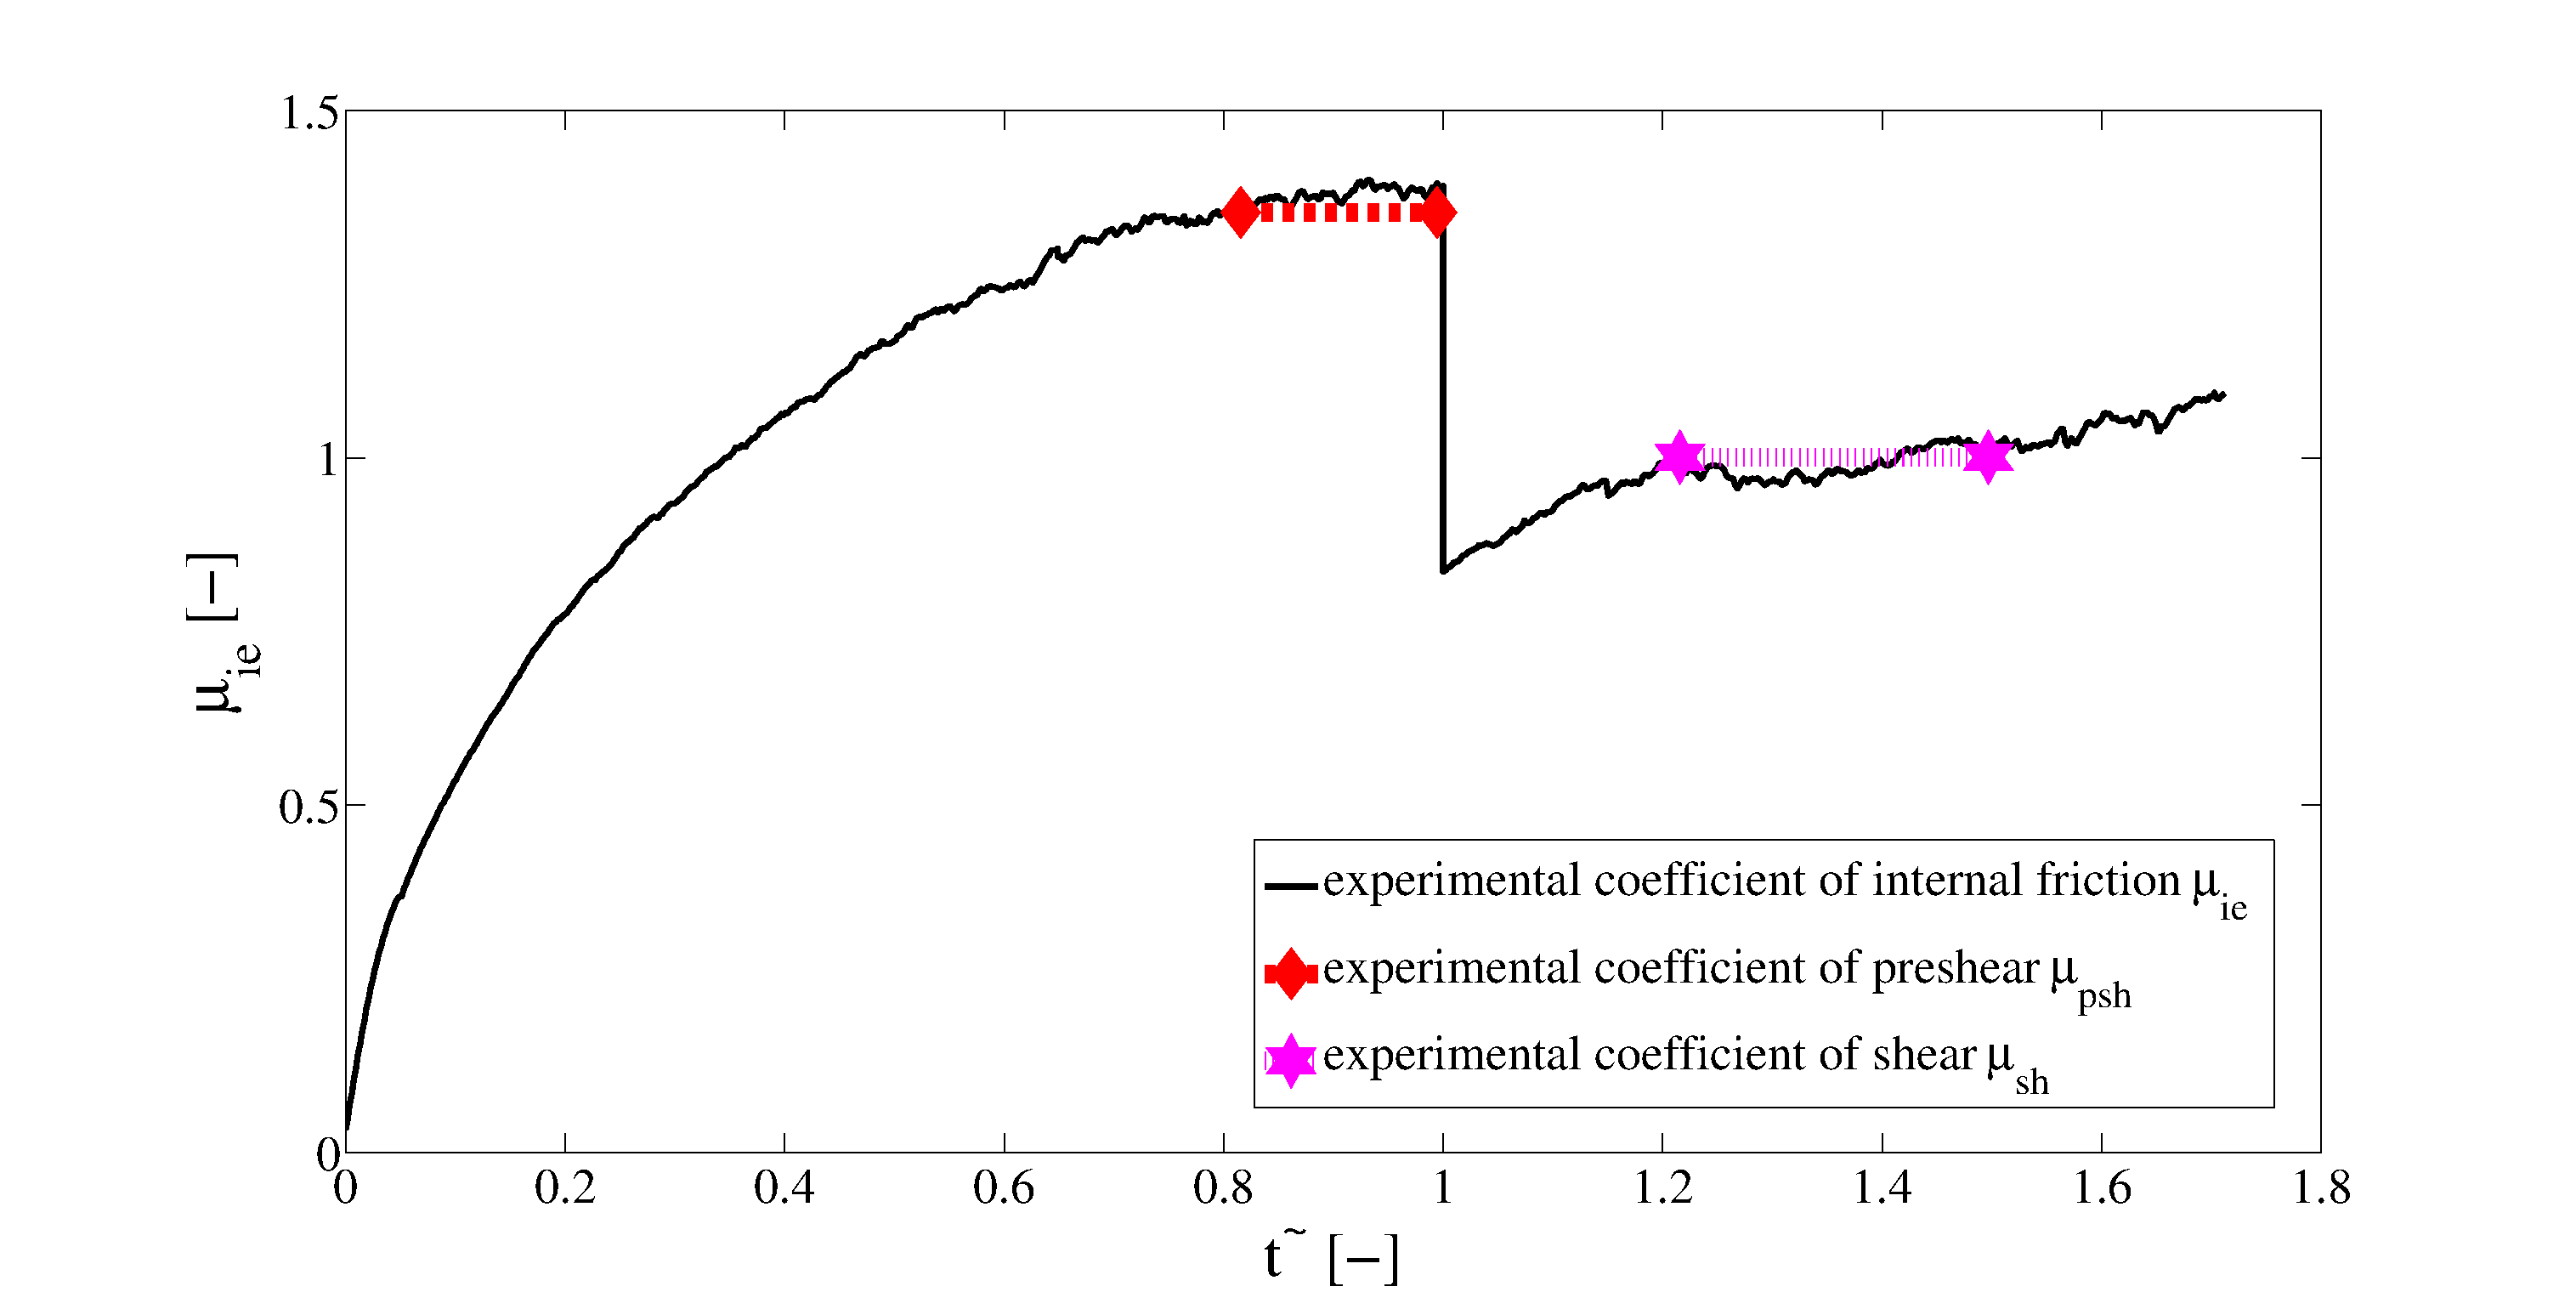
\includegraphics[width=\textwidth]{images/original/20experimental}
        \caption{Experimental shear cell tester stress path - $\sigma_n = 2000
        [Pa]$}
        \label{fig:20experimental} 
    \end{subfigure}\\
        \begin{subfigure}[b]{2cm}
        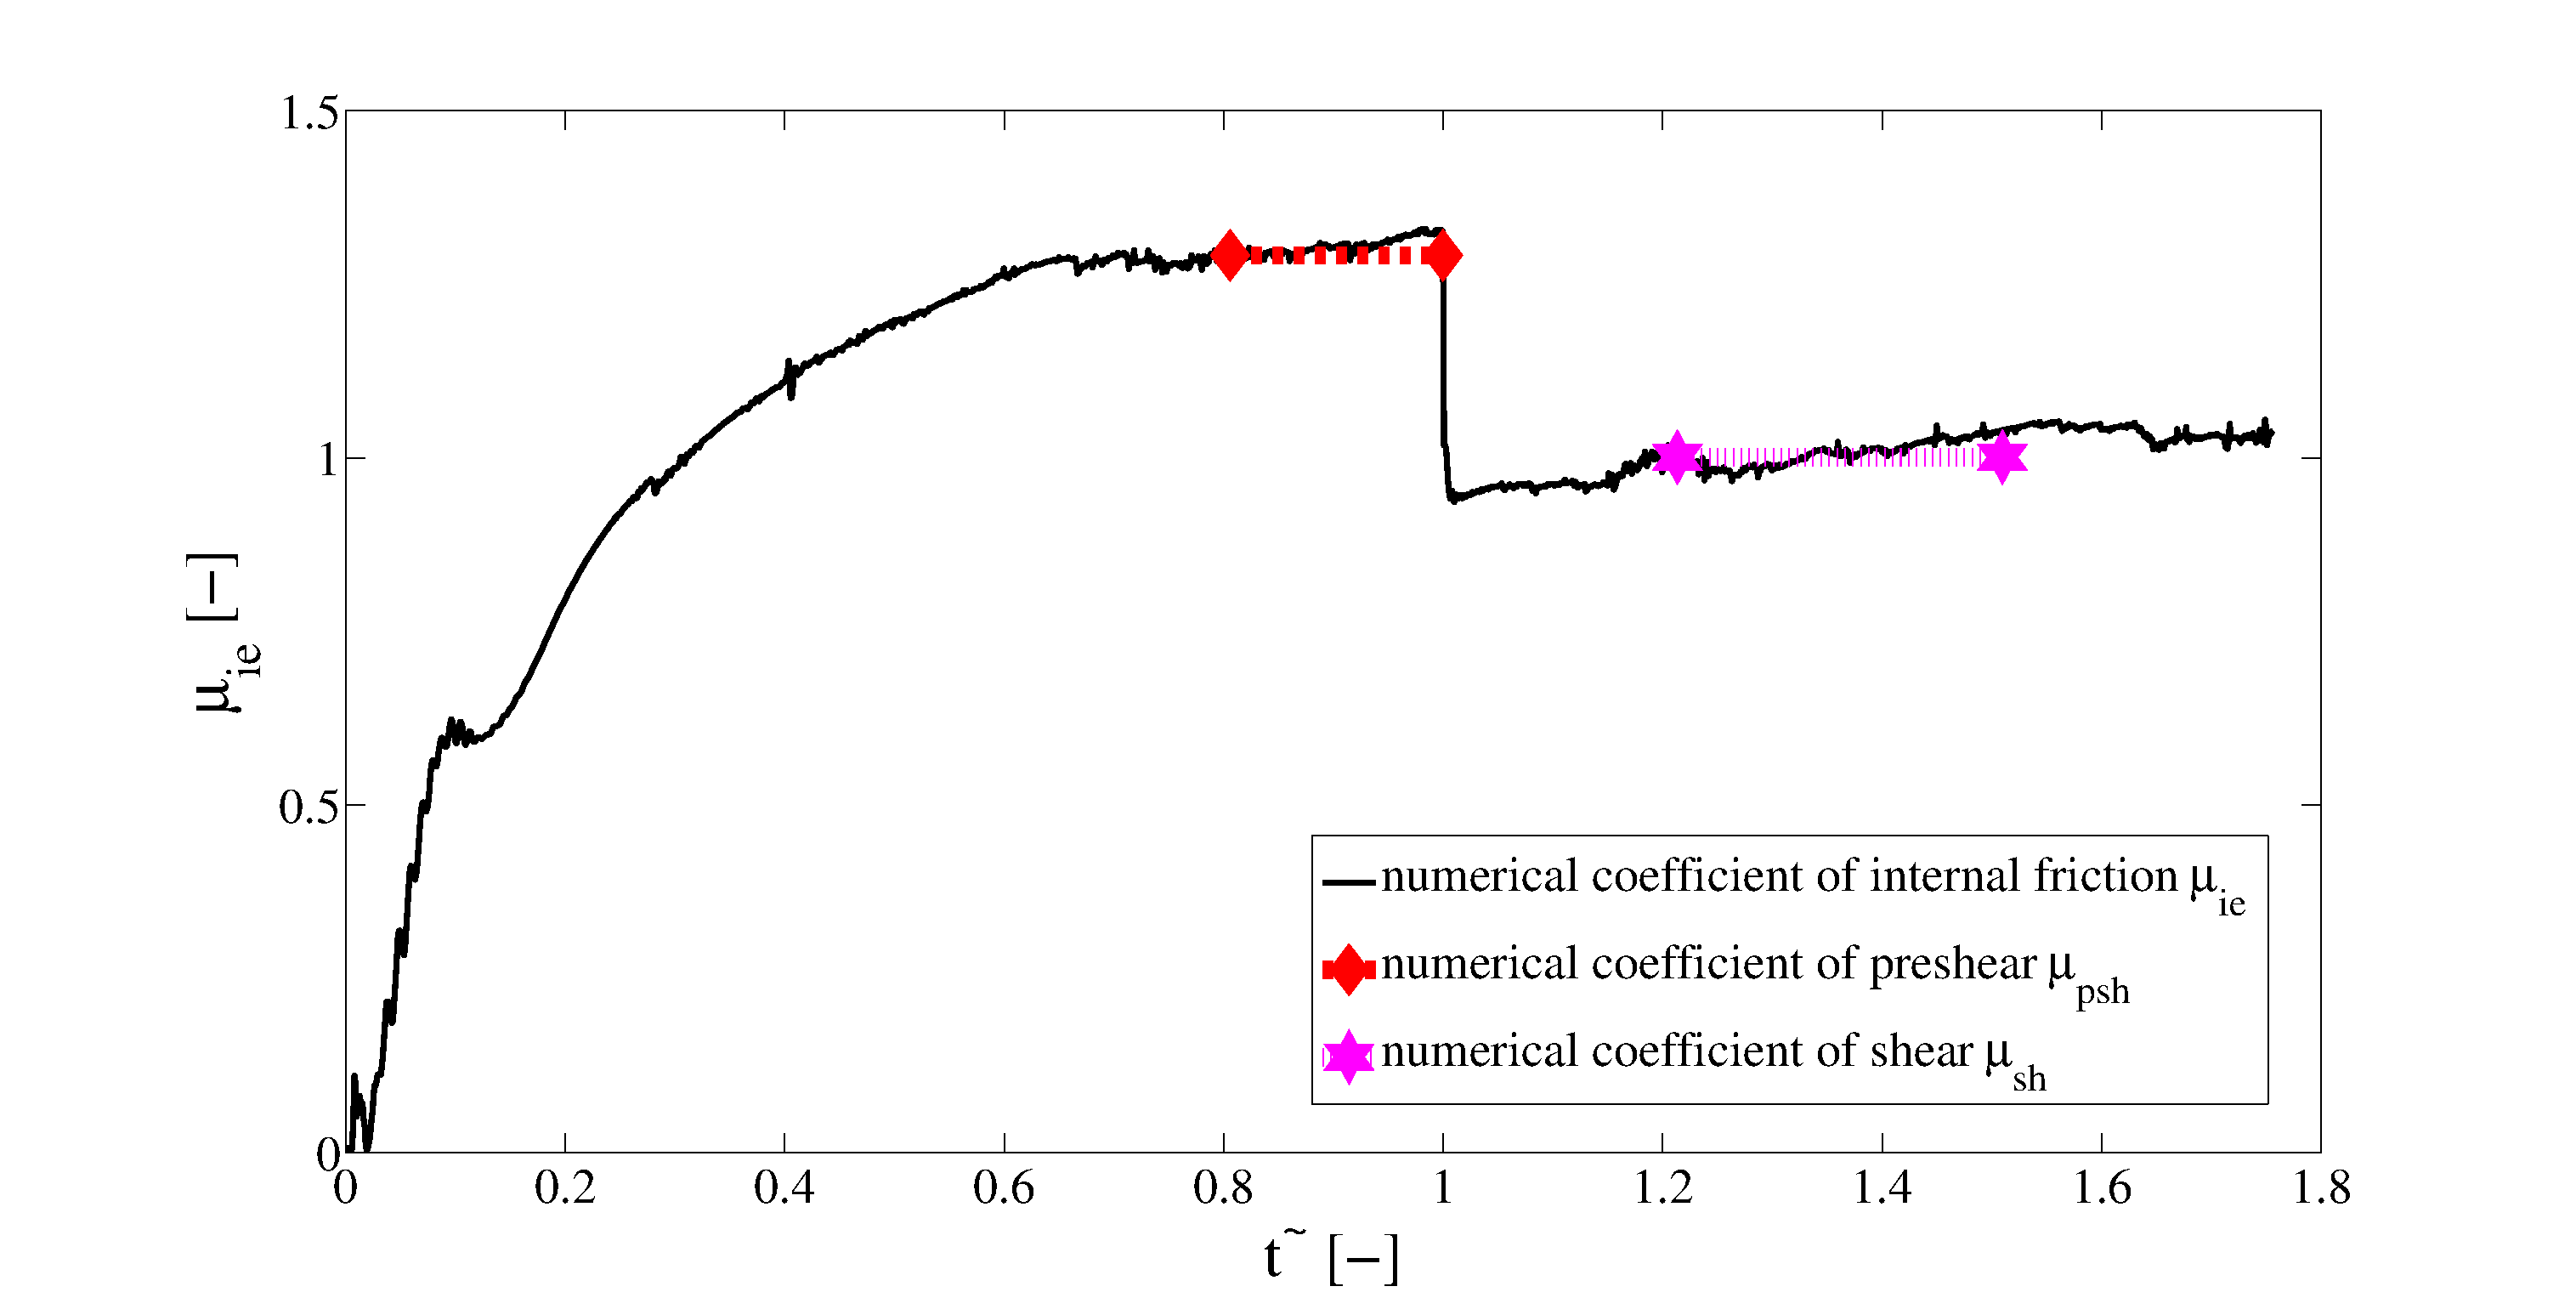
\includegraphics[width=\textwidth]{images/original/21simexample}
        \caption{Numerical shear cell tester stress path - $\sigma_n = 10000
        [Pa]$}
        \label{fig:21simexample} 
    \end{subfigure}
    \caption[Stress path]{Sample of the stress path for
	the Schulze ring shear cell tester, experimental and numerical.
	Time is normalized: $\tilde{t} = t/t_{change}$, where $t_{change}$ is the
	time when the normal stress ($\sigma_n$) is modified during the tests.
	Until $\tilde{t}=1$ the $\sigma_n = 2000 ~[Pa]$ is kept constant. 
	In Fig. \ref{fig:20experimental} at $\tilde{t}~=0.91$
 	a plateau is reached.
	The $\mu_{psh}$ is calculated as average of the $\mu_{ie}$ in this first
	plateau.
	Later, at $\tilde{t}=1$, the $\sigma_n$ is reduced to $80 \%$ of its initial
	value.
	Soon, a second plateau starts.
	As average of $\mu_{ie}$ in this second plateau we obtain $\mu_{sh}$.
	The stress path is in the numerical simulation is comparable to the
	experimental one, especially the plateaux.
	They were clearly relevant because there we collected the numerical bulk
	behaviour representative values. }
    \label{fig:40experimentalsimulation}
\end{figure}

\begin{table}[h]
\centering
\begin{tabular}{cccccc}
\hline
$\sigma_n$ (Pa) & $\tau$ (Pa) & $\mu_{psh}$ (-) & $\tau_{\%}$ (\%) &
$\mu_{sh}$ (-) & $\rho_b$ (kg/m3) \\
\hline
    1068  & 1059  & 0.9916 & 80 & 1.2333 & 1718 \\
    2069  & 1818  & 0.8787 & 80 & 0.9994 & 1759 \\
    10070 & 8232  & 0.8175 & 80 & 1.1712 & 1802 \\

\hline
\end{tabular}
\caption[Experimental results]{Experimental results. Values for three
load conditions}
\label{tab:05sinterTableExperimental}
\end{table}

\subsection{DEM Simulations}
\label{subsec:simulations}

For sinter fine 546 shear cell and 81 static angle of repose simulations have
been realized with the variations described in table
\ref{tab:10DEMVariableinputvalues}.
A representative stress path can be seen in Fig. \ref{fig:21simexample}.
Although the duration is smaller by two order of magnitude, the stress path is
comparable to the experimental one, especially the plateaux.
They were clearly relevant because there we collected the numerical bulk
behaviour representative values.\\
The computational time resulted in 1 hour with 32 AMD cores for a benchmark
shear cell simulation and 9 hours for a benchmark $AOR$ simulation, both with 50K particles. 
Simulations with large $dCylDp$ required a greater time amount (e.g. with 400K
particles about 12 hours for the shear cell). \\
%\begin{figure}[!htb] 
\centering 
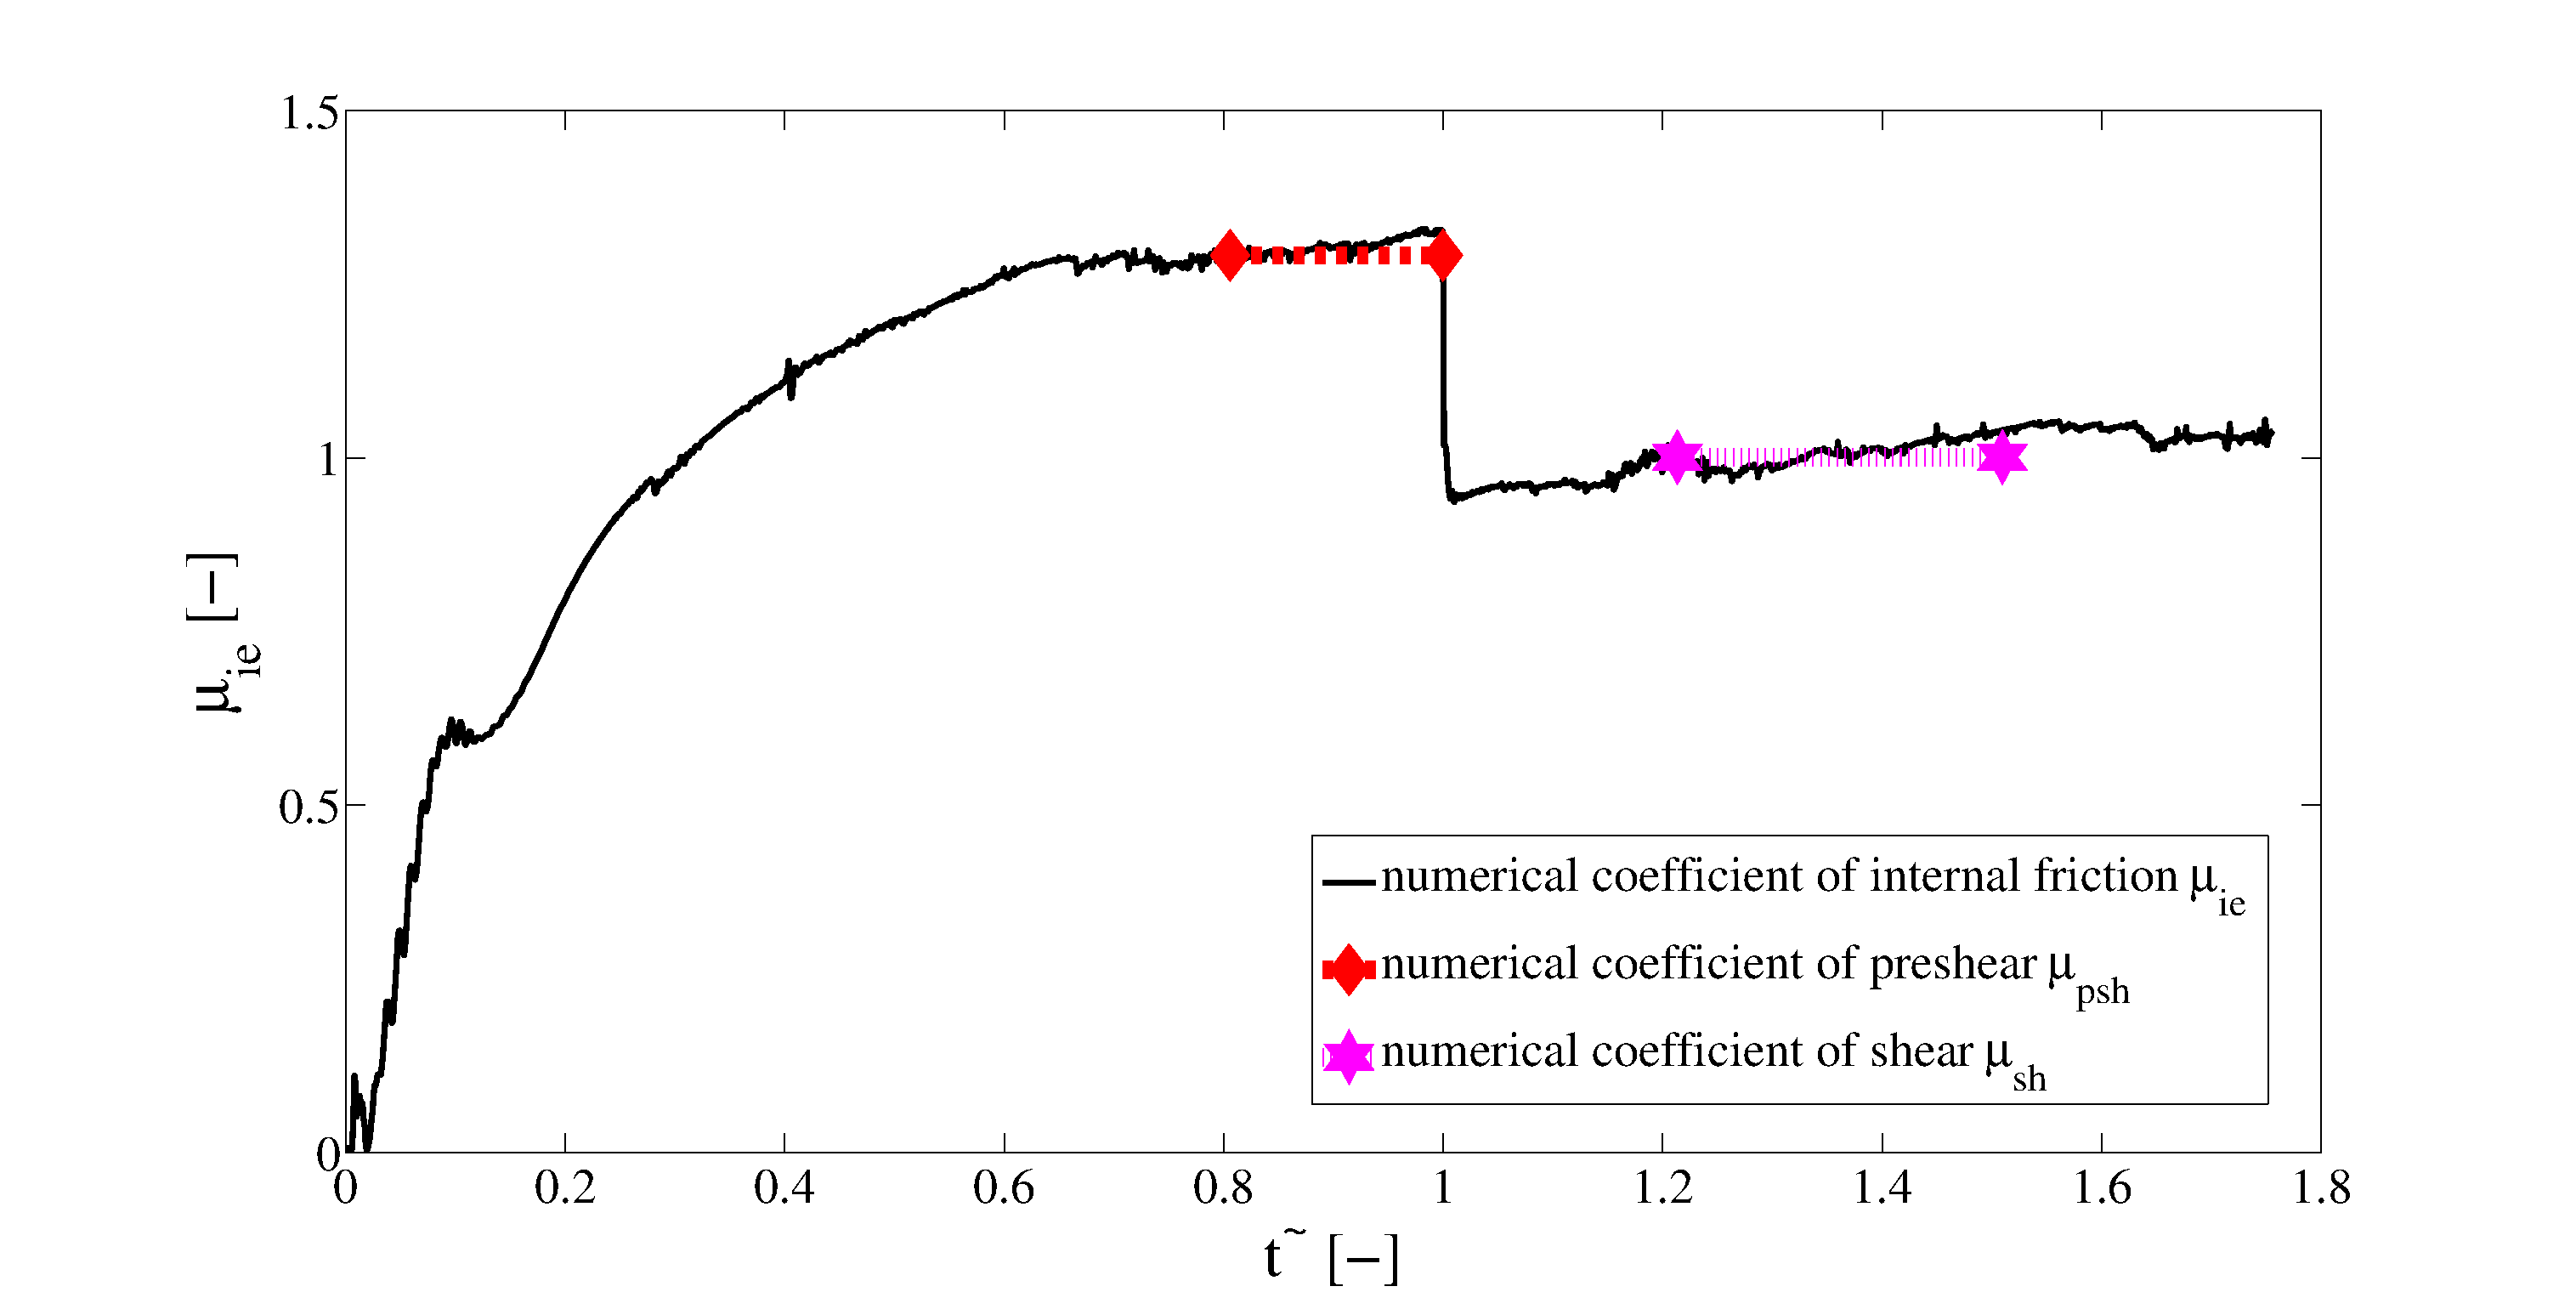
\includegraphics[width=.96\textwidth]{images/original/21simexample} 
\caption{Numerical stress path}
\label{fig:21simexample} 
\end{figure}


% \begin{figure}[htp]
%     \centering
%     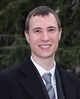
\includegraphics[width=.2\textwidth]{images/vitae/lbenvenuti}
%     \caption{OpenMP, MPI, MPI/OpenMP Hybrid runs of Box in a box testcase on 32
%     cores. The OpenMP-only run suffers from limited memory bandwidth in
%     memory-bound algorithms inside of the Modify section of the code. MPI-only has
%     low averaged runtimes for each section, but a very large Other timing, which
%     hints for a large amount of load-imbalance. Hybrid timings are a bit worse
%     on average, but because of better balancing, processes have lower wait times
%     inside of Other timing.}
% 	\label{fig:boxInBoxComparison}


\subsection{ANN model development}
\label{subsec:annmodeldev}

First, we controlled the regression of the bulk behaviour parameters, e.g. the
$\mu_{psh}$, see Fig. \ref{fig:22regression}, where the corresponding plot for
the $NN$ with the maximum $R^2$ in shown. Each circle represents one of the 546
simulations.
The plot presents a consistent agreement between the $DEM$ results distribution
(T in the legend) and the $NN$ regression (or fitting) line.
% \begin{figure}%[!h] 
\centering 
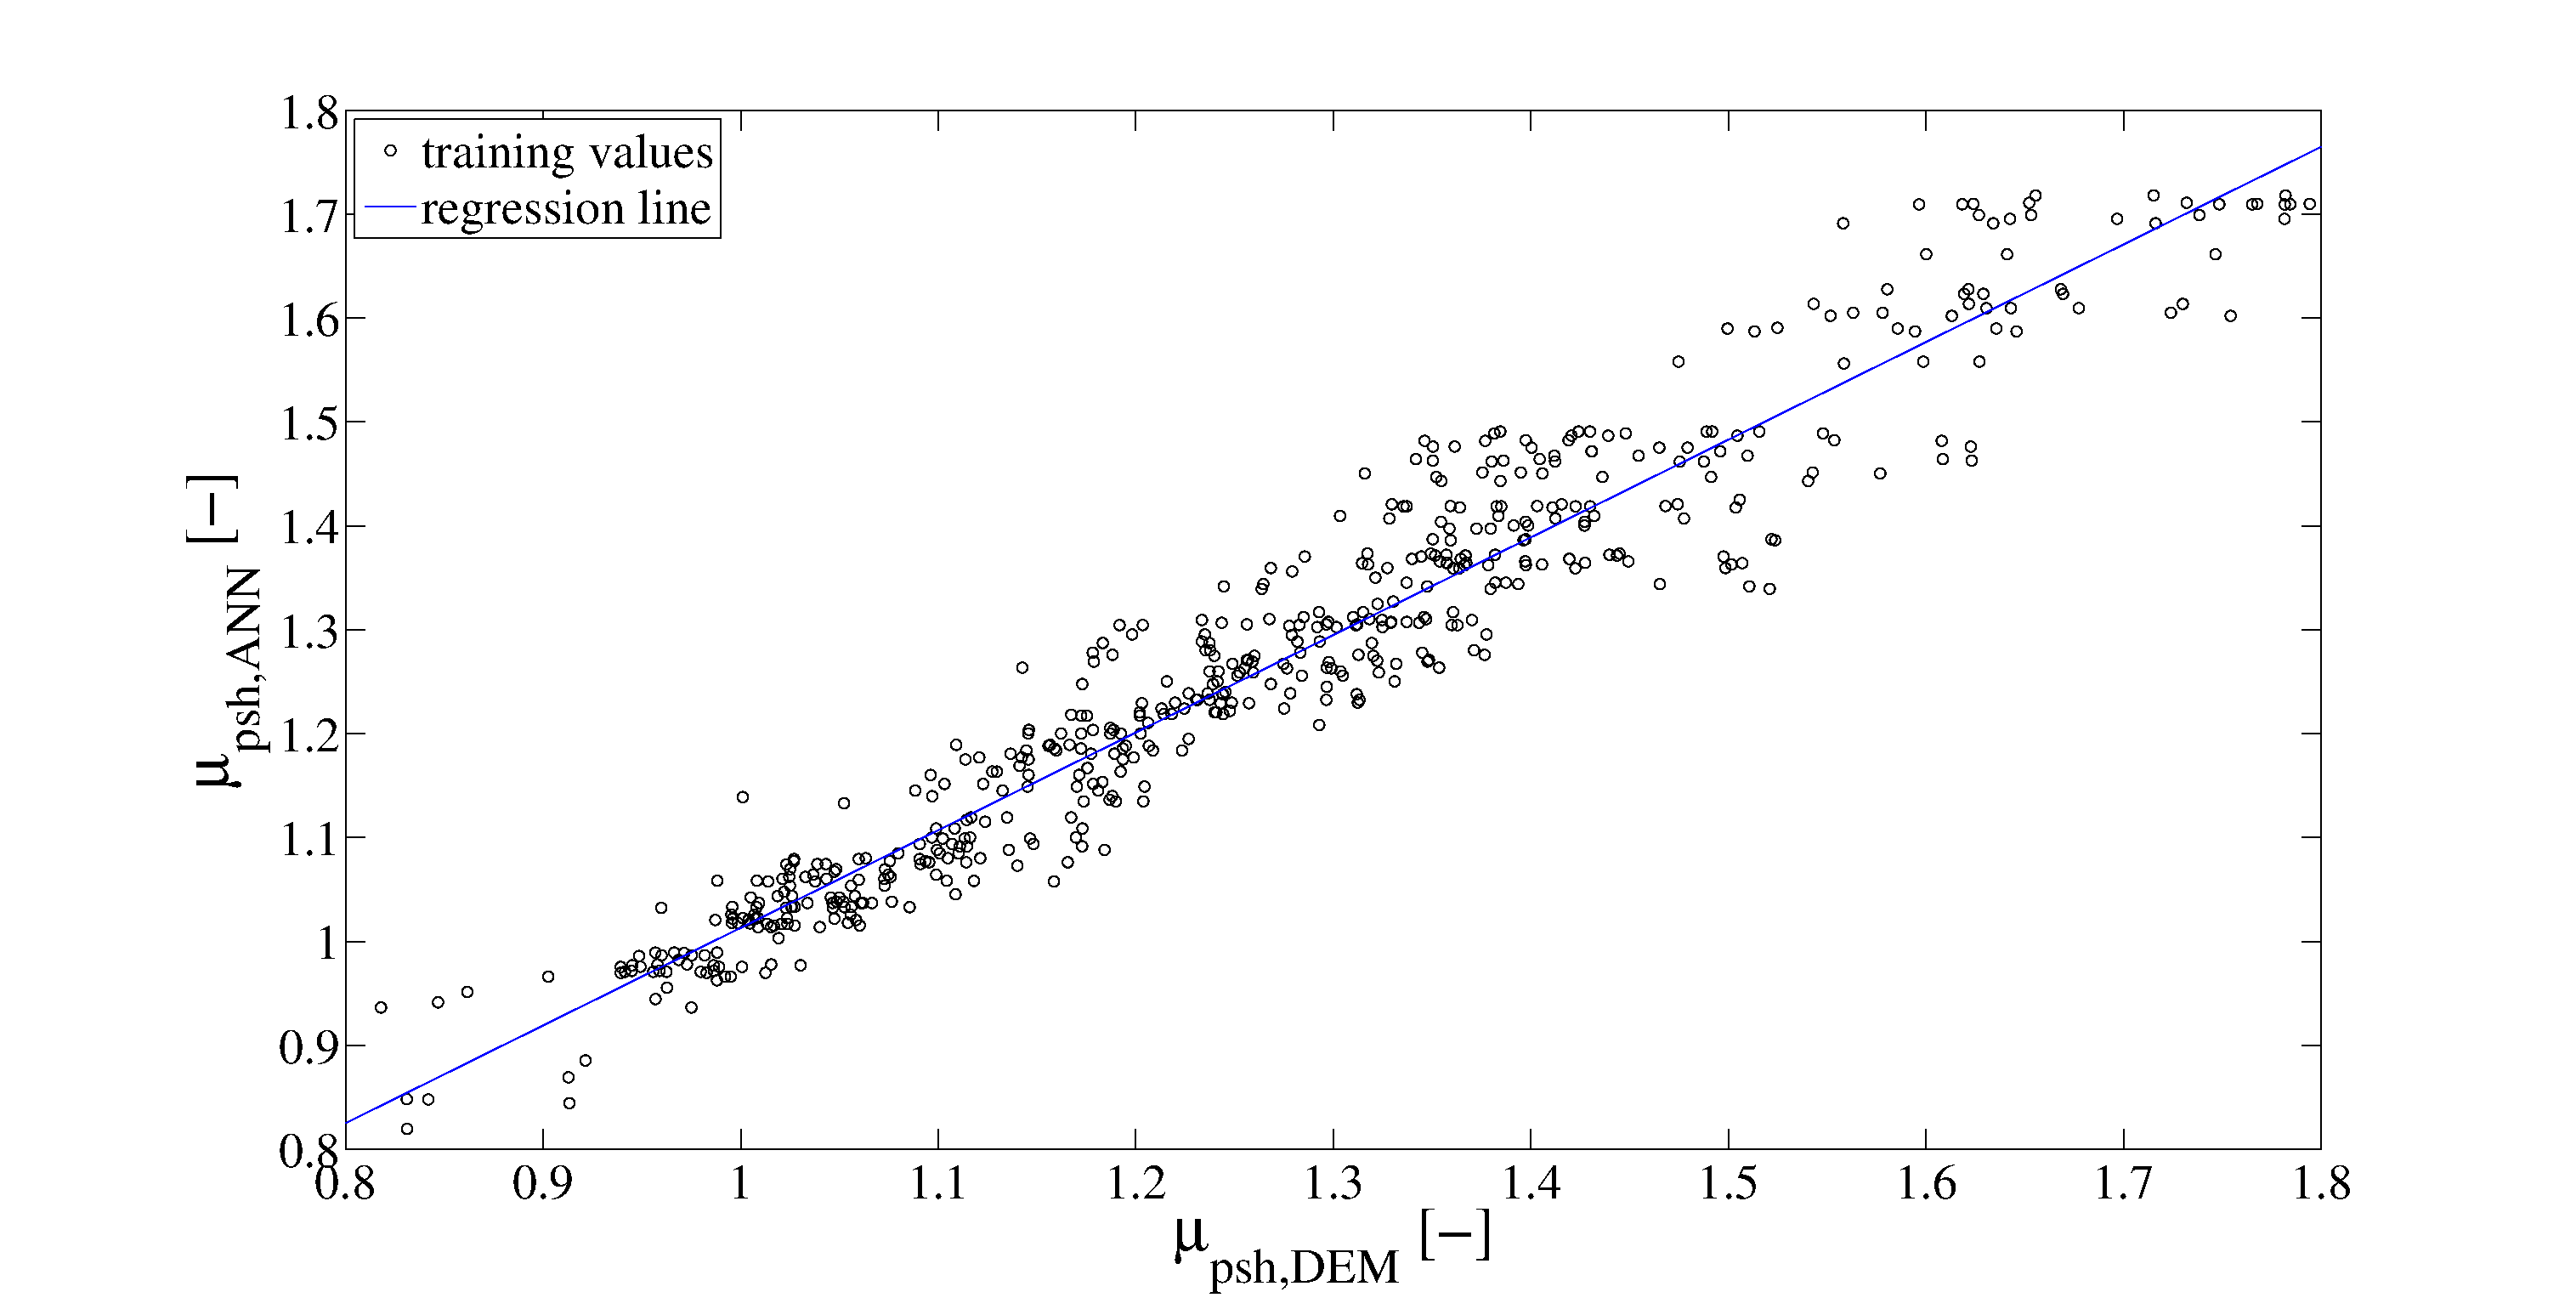
\includegraphics[width=.96\columnwidth]{images/22regression.eps}
%[width=.96\textwidth]
\caption[Comparison between prediction of the trained ANN and full DEM
simulation]{Comparison between prediction of the trained Artificial Neural
Network ($ANN$) and 546 
\wrong{write down all the simulations performed at the end.}
full DEM simulations of the coefficient of pre-shear
($\mu_{psh}$).}
\label{fig:22regression} 
\end{figure}
The linear relationship between the
training values have been evaluated in Table \ref{tab:06inputRelationshipTable}.
The clearest connections were between $\mu_s$ and $\mu_{psh}$, and
$\rho_p$ and $\rho_b$.
Instead, for $\mu_{sh}$ and $AOR$ the $\mu_r$ balanced the influence of the 
$\mu_s$, and further parameters were worthly correlated. \\
% \begin{table}[h]
\centering
\scalebox{1.0}{
\begin{tabular}{c|cccccccc}
\hline
          & $\mu_s$ & $\mu_r$ & $COR$ & $\rho_p$ & $\mu_{sh}$ & $\mu_{psh}$ & $\rho_{b}$ & $AOR$ \\
          \hline
    $\mu_s$ & 100.00 & 0.55  & 0.04  & 0.00  & 3.84  & 87.26 & 8.39  & 49.48 \\
    $\mu_r$ & 0.55  & 100.00 & 0.15  & 0.00  & 58.92 & 33.70 & 3.10  & 60.20 \\
    $COR$ & 0.04  & 0.15  & 100.00 & 0.00  & 15.52 & 0.57  & 1.71  & 0.00 \\
    $\rho_p$ & 0.00  & 0.00  & 0.00  & 100.00 & 4.98  & 5.71  & 99.00 & 0.00 \\
    $\mu_{sh}$ & 3.84  & 58.92 & 15.52 & 4.98  & 100.00 & 26.03 & 9.52  & 0.00 \\
    $\mu_{psh}$ & \textbf{87.26} & 33.70 & 0.57  & 5.71  & 26.03 & 100.00 & 4.33 
    & 0.00
    \\
    $\rho_{b}$ & 8.39  & 3.10  & 1.71  & \textbf{99.00} & 9.52  & 4.33  & 100.00
    & 0.00 \\
    $AOR$ & 49.48 & \textbf{60.20} & 0.00  & 0.00  & 0.00  & 0.00  & 0.00  &
    100.00 \\
    
\hline
\end{tabular}}
\caption{Values of linear relationship between considered variables multiplied
for 100}
\label{tab:06inputRelationshipTable}
\end{table}
Then we observed how the $R^2$ changed with the different number of neurons for
the $\mu_{psh}$.
Then we observed how the $R^2$ changed with the different number of neurons for the $\mu_{psh}$. 
In this case we reached a $R^2 = 0.96$ for a $NN$ with fifteen neurons. 
Increasing the number of neurons did not improve the $R^2$, that even started to oscillate with the neuron number. 
Later, we processed the random combinations (table
\ref{tab:10DEMVariableinputvalues}) with the $NN$.
The $NN$ evaluation was incredibly faster compared to the $DEM$ simulations. The
individuation of all the tabbed $DEM$ combinations for the shear cell did not take more than a few seconds on a single core. 
We represented the tabbed combinations ($TC1$) for one load condition of the
shear cell ($\sigma_n=10070 ~[Pa]$, $P=1.0$) in Fig.
\ref{fig:24radarpirker1schulze10070}.
% \begin{figure}[htp] \centering
    \begin{subfigure}[b]{0.48\columnwidth}
        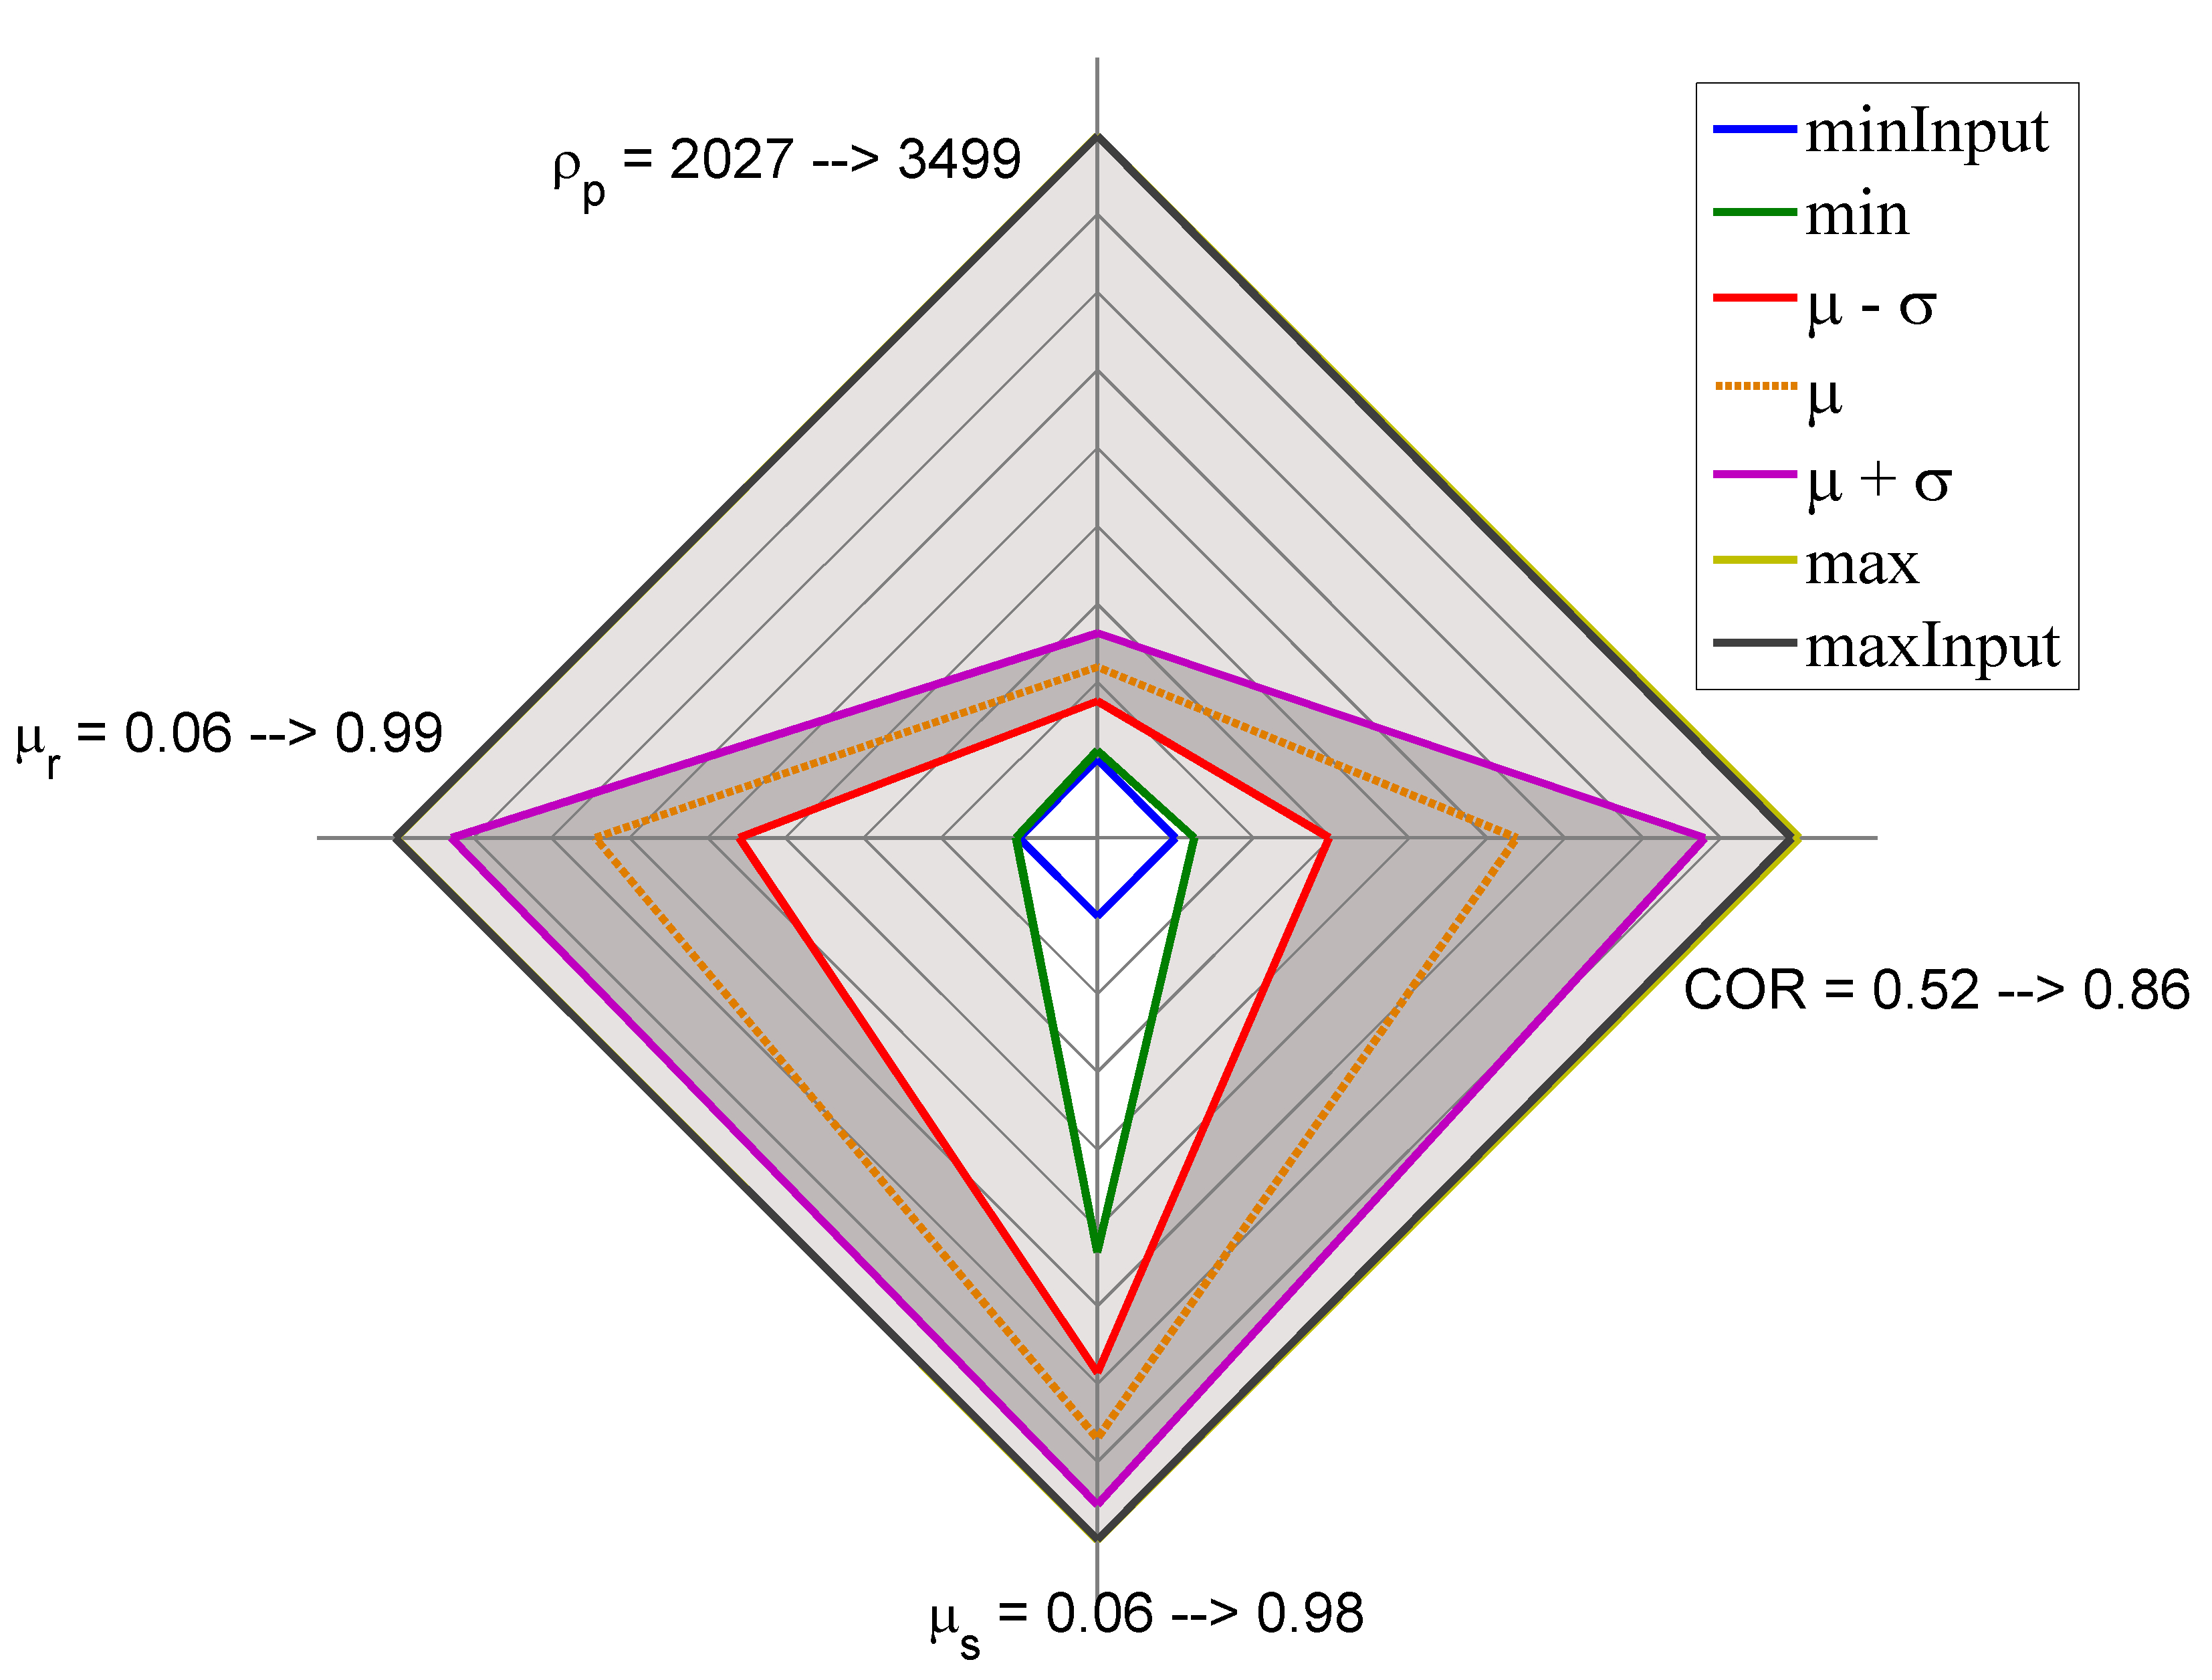
\includegraphics[width=\textwidth]{images/original/24radarpirker1schulze10070}
        \caption{Radar P1 Schulze10070}
        \label{fig:24radarpirker1schulze10070}
    \end{subfigure}
    \begin{subfigure}[b]{0.48\columnwidth}
        \includegraphics[width=\textwidth]{images/original/25cloudpirker1schulze10070}
        \caption{Cloud P1 Schulze10070}
        \label{fig:25cloudpirker1schulze10070}
    \end{subfigure}\\
        \begin{subfigure}[b]{0.48\columnwidth}
        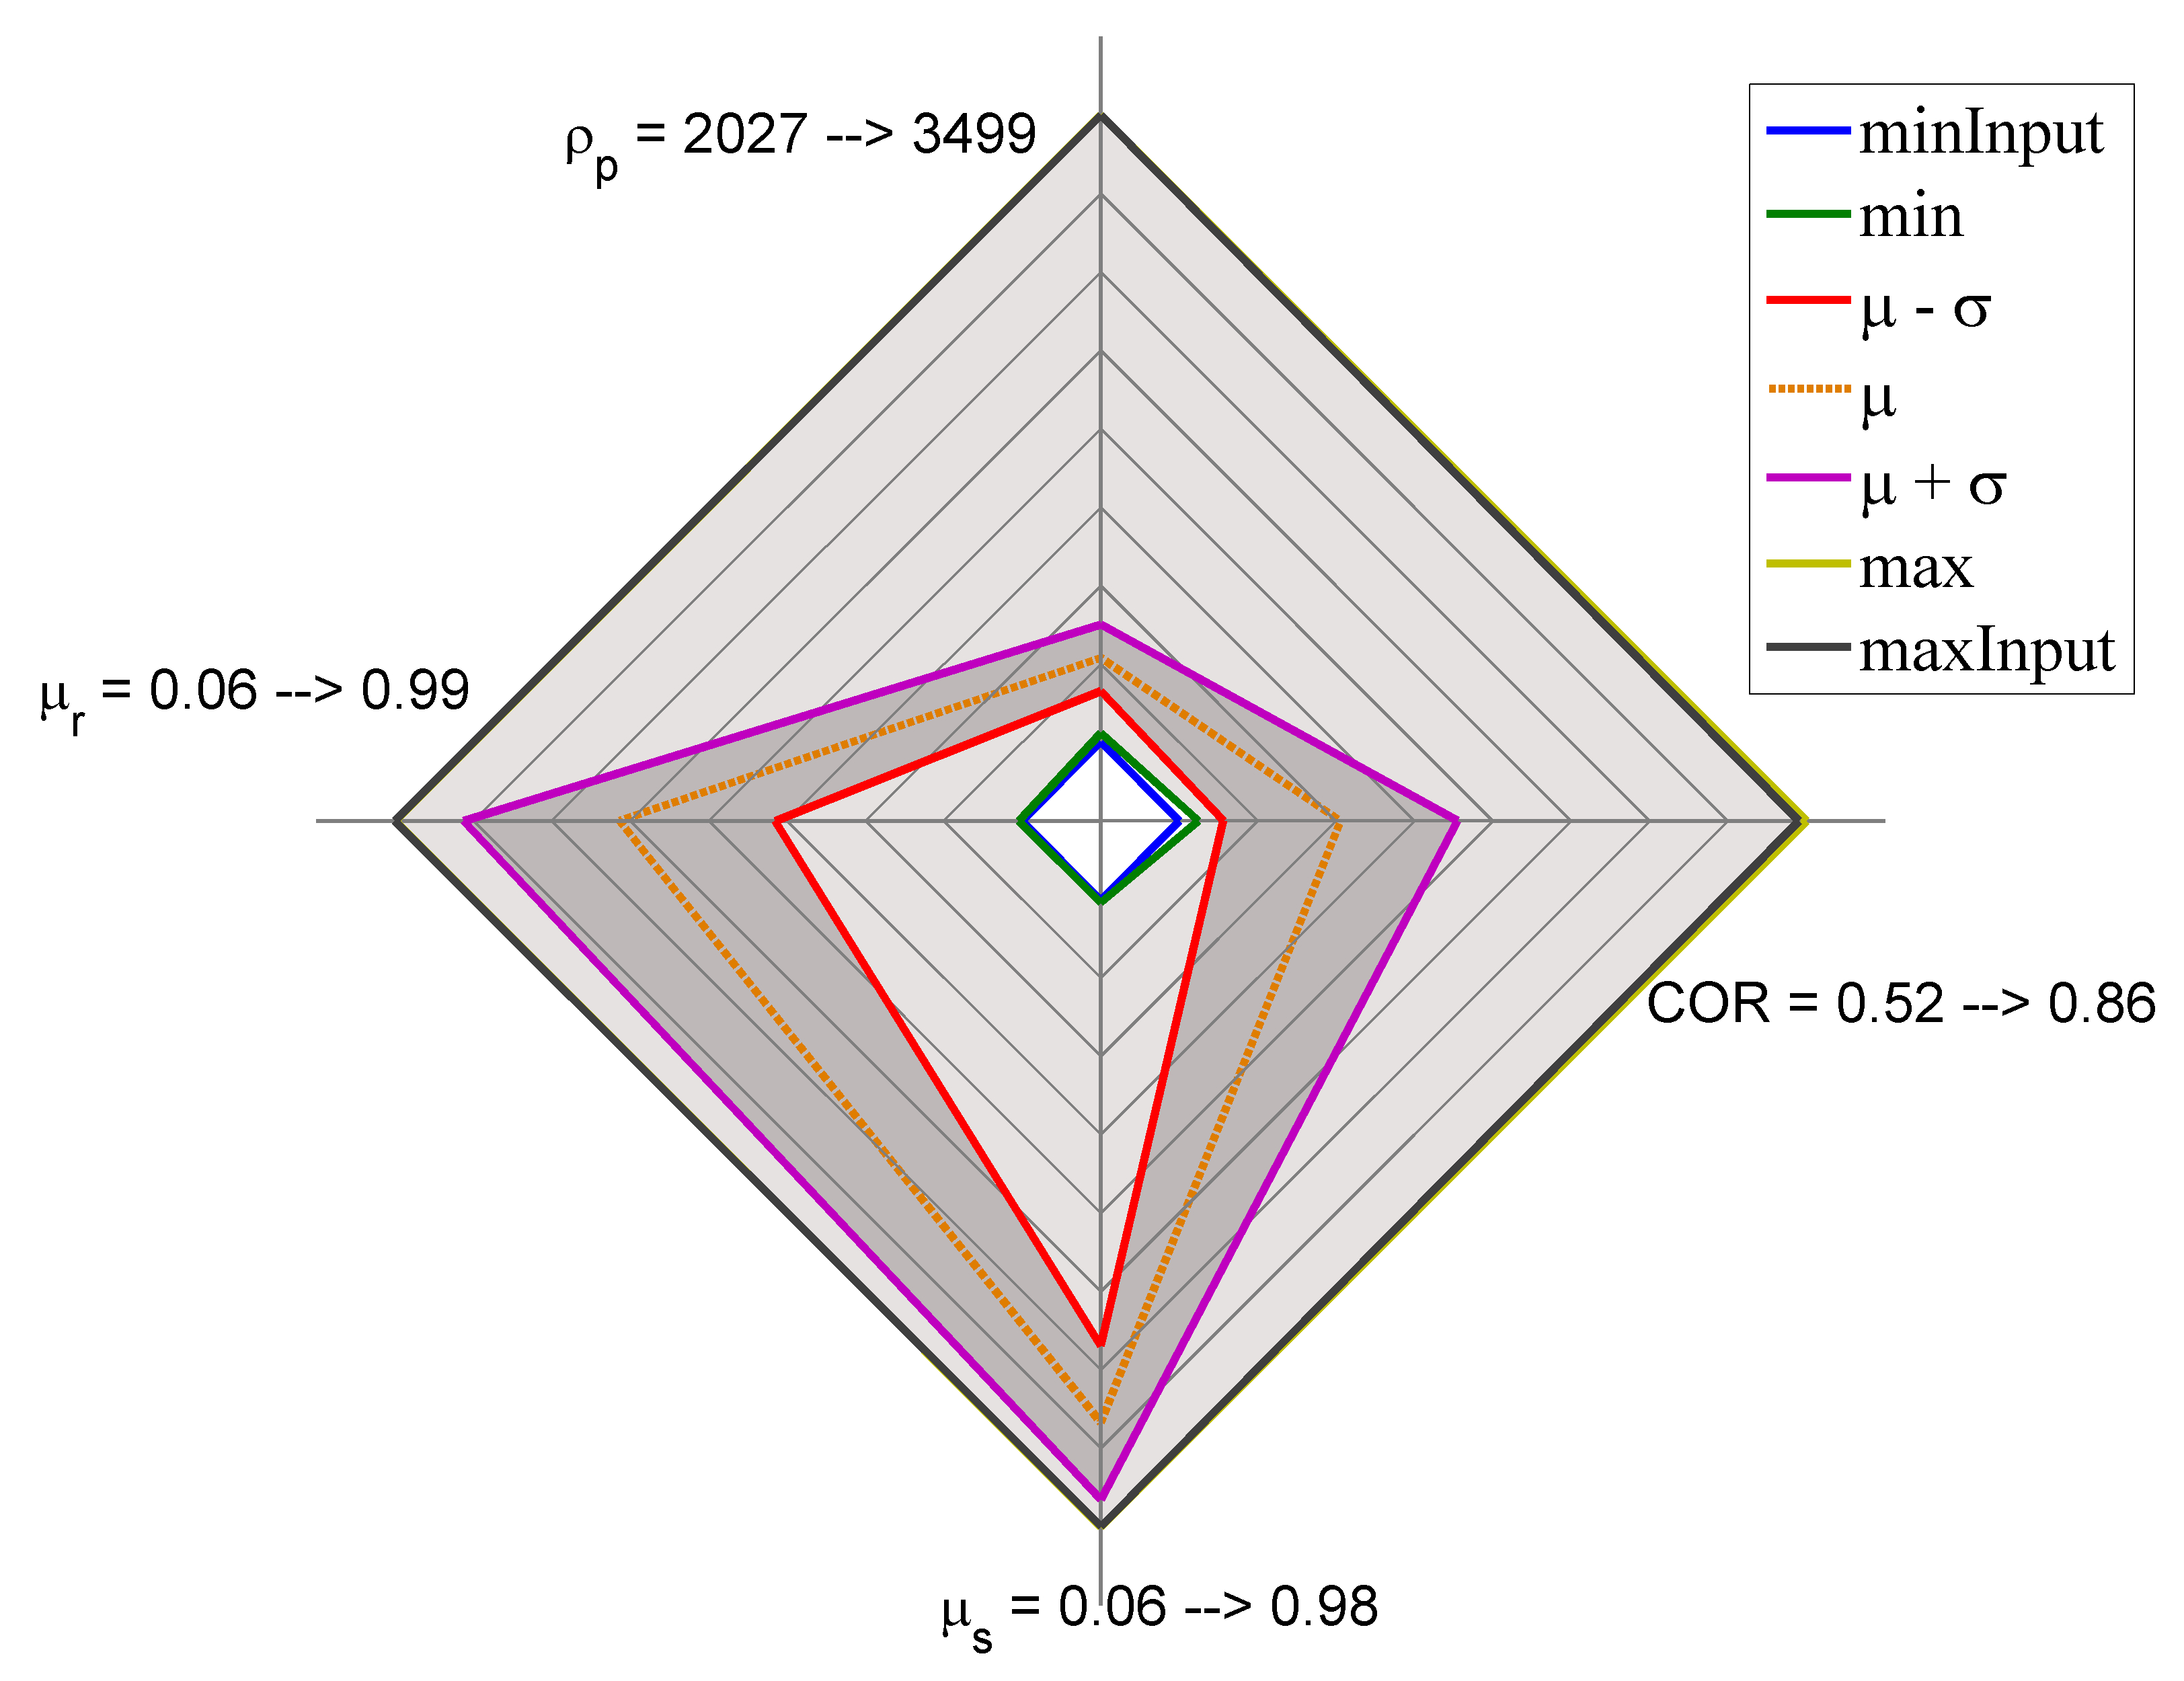
\includegraphics[width=\textwidth]{images/original/26radarpirker08schulze10070}
        \caption{Radar P08 Schulze10070}
        \label{fig:26radarpirker08schulze10070} 
    \end{subfigure}
    \begin{subfigure}[b]{0.48\columnwidth}
        \includegraphics[width=\textwidth]{images/original/27cloudpirker08schulze10070}
        \caption{Cloud P08 Schulze10070}
        \label{fig:27cloudpirker08schulze10070} 
    \end{subfigure}\\
        \begin{subfigure}[b]{0.48\columnwidth}
        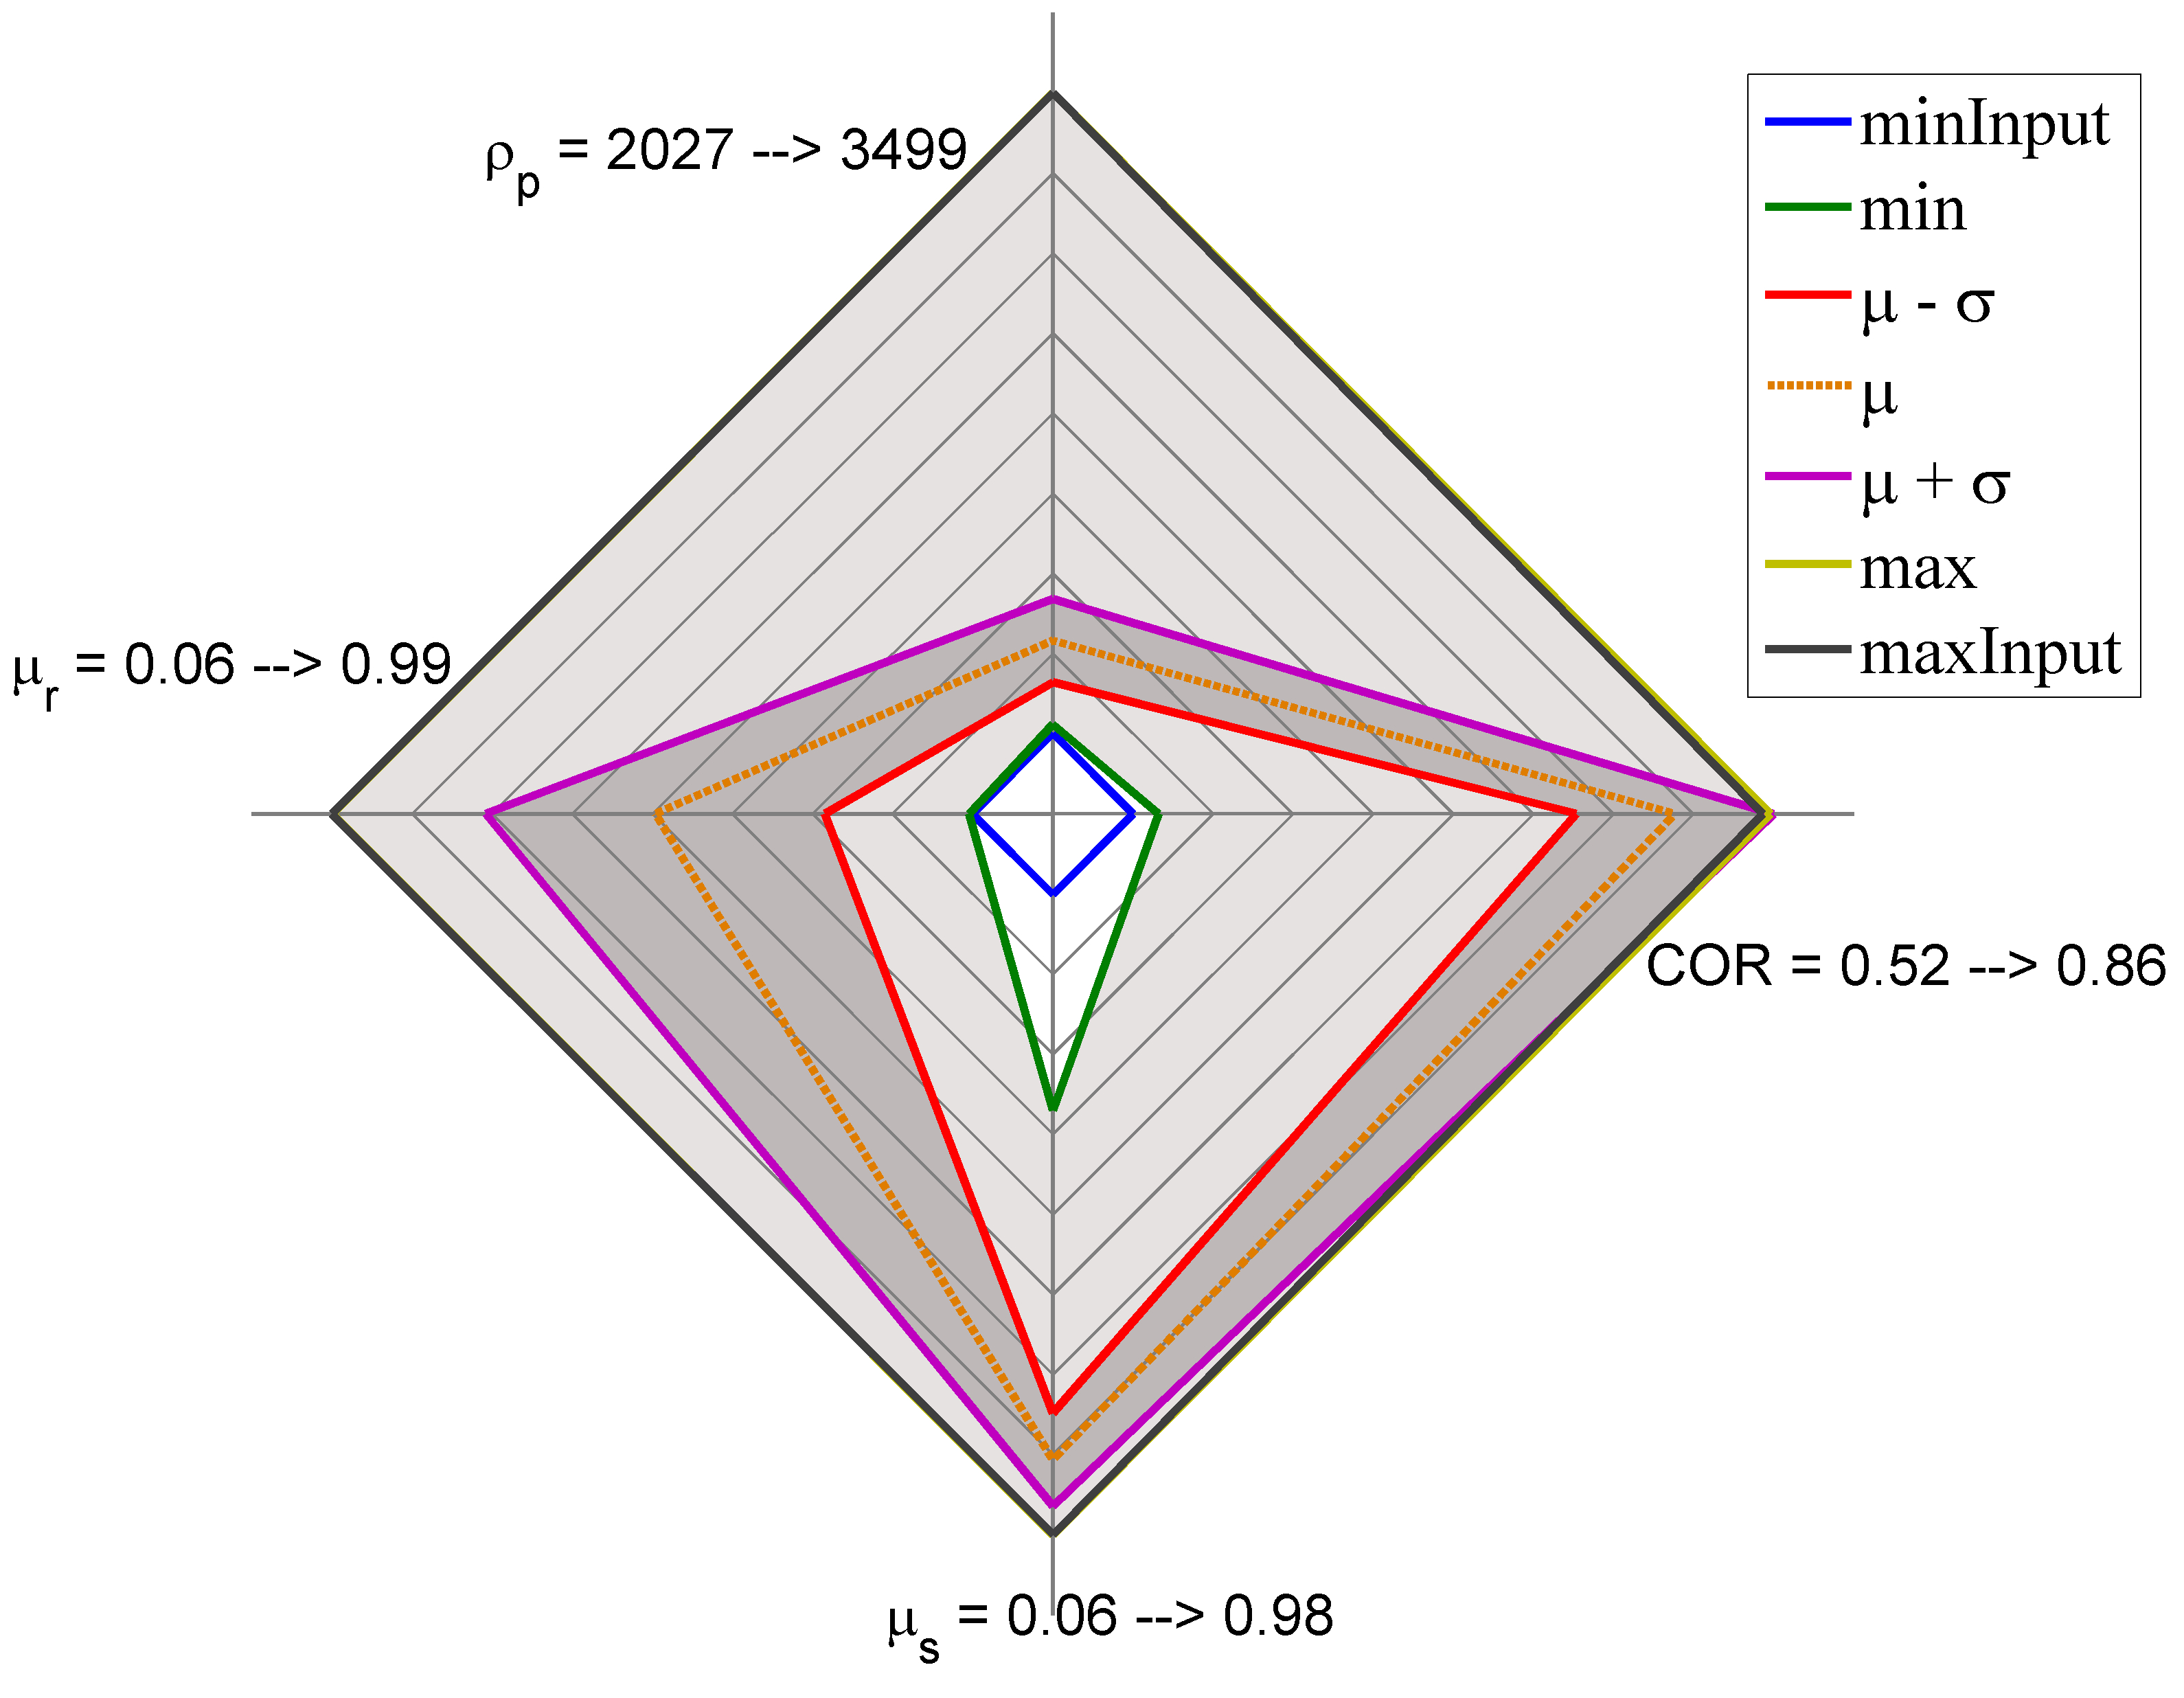
\includegraphics[width=\textwidth]{images/original/28radarpirker12schulze10070}
        \caption{Radar P12 Schulze10070}
        \label{fig:28radarpirker12schulze10070} 
    \end{subfigure}
    \begin{subfigure}[b]{0.48\columnwidth}
        \includegraphics[width=\textwidth]{images/original/30cloudpirker12schulze10070}
        \caption{Cloud P12 Schulze10070}
        \label{fig:30cloudpirker12schulze10070} 
    \end{subfigure}
    \caption{Comparison between the original experimental selection P=1 and the
    increased and decreased results.}
    \label{fig:29schulzeradarandcloud}
\end{figure}
Here, the minimum and maximum values, together with the mean and the confidence
range, provided by the square deviation, are shown. Notably, the confidence range is large, 
especially for the $COR$, highlighting its scarce influence over the characterization. 
Instead, both the $\rho_p$  and the $\mu_s$ show a narrow confidence range, 
displaying at the same time their influence and the validity of this procedure to find valid $DEM$ parameters. 
That agrees with the examination of the ratio of the standard deviation to the
range, see table \ref{tab:13DEMvalidvalues}.
Further, we could see how different $DEM$ parameters
combinations could reproduce the experimental behaviour and evaluate their mutual dependencies. 
This is clearer in a cloud plot, as in Fig. 
\ref{fig:25cloudpirker1schulze10070}. While the $COR$ varied, multiple
combinations ($250407 --> 4\% $ of the total) of $\mu_s$ and $\mu_r$ reproduced
the experimental behaviour.
This underlines once more their correlation, as already stated by Wensrich and 
Katterfeld \cite{RefWorks:87}.
To further demonstrate the validity of the procedure, we modified the product
coefficient. In the first attempt we set it to $P=0.8$ and we obtained another
series of tabbed combinations ($TC2$).
We can see in the radar plot in Fig.
\ref{fig:26radarpirker08schulze10070} that the confidence range is narrower
compared to $P=1.0$, while in the cloud plot in Fig. 
\ref{fig:27cloudpirker08schulze10070} the area
appears larger, although slightly less densely populated. Finally, for $P=1.2$
and its tabbed combinations ($TC3$) the radar plot in Fig.
\ref{fig:28radarpirker12schulze10070} shows a largely different confidence
range, while the cloud plot in Fig. \ref{fig:30cloudpirker12schulze10070} 
illustrates a smaller area. As expected, the procedure was highly sensible to the variations of the experimental data. 
Thus, it could be effectively handled for a wide range of bulk materials.\\
% \begin{figure}[htp] \centering
    \begin{subfigure}[b]{0.48\columnwidth}
        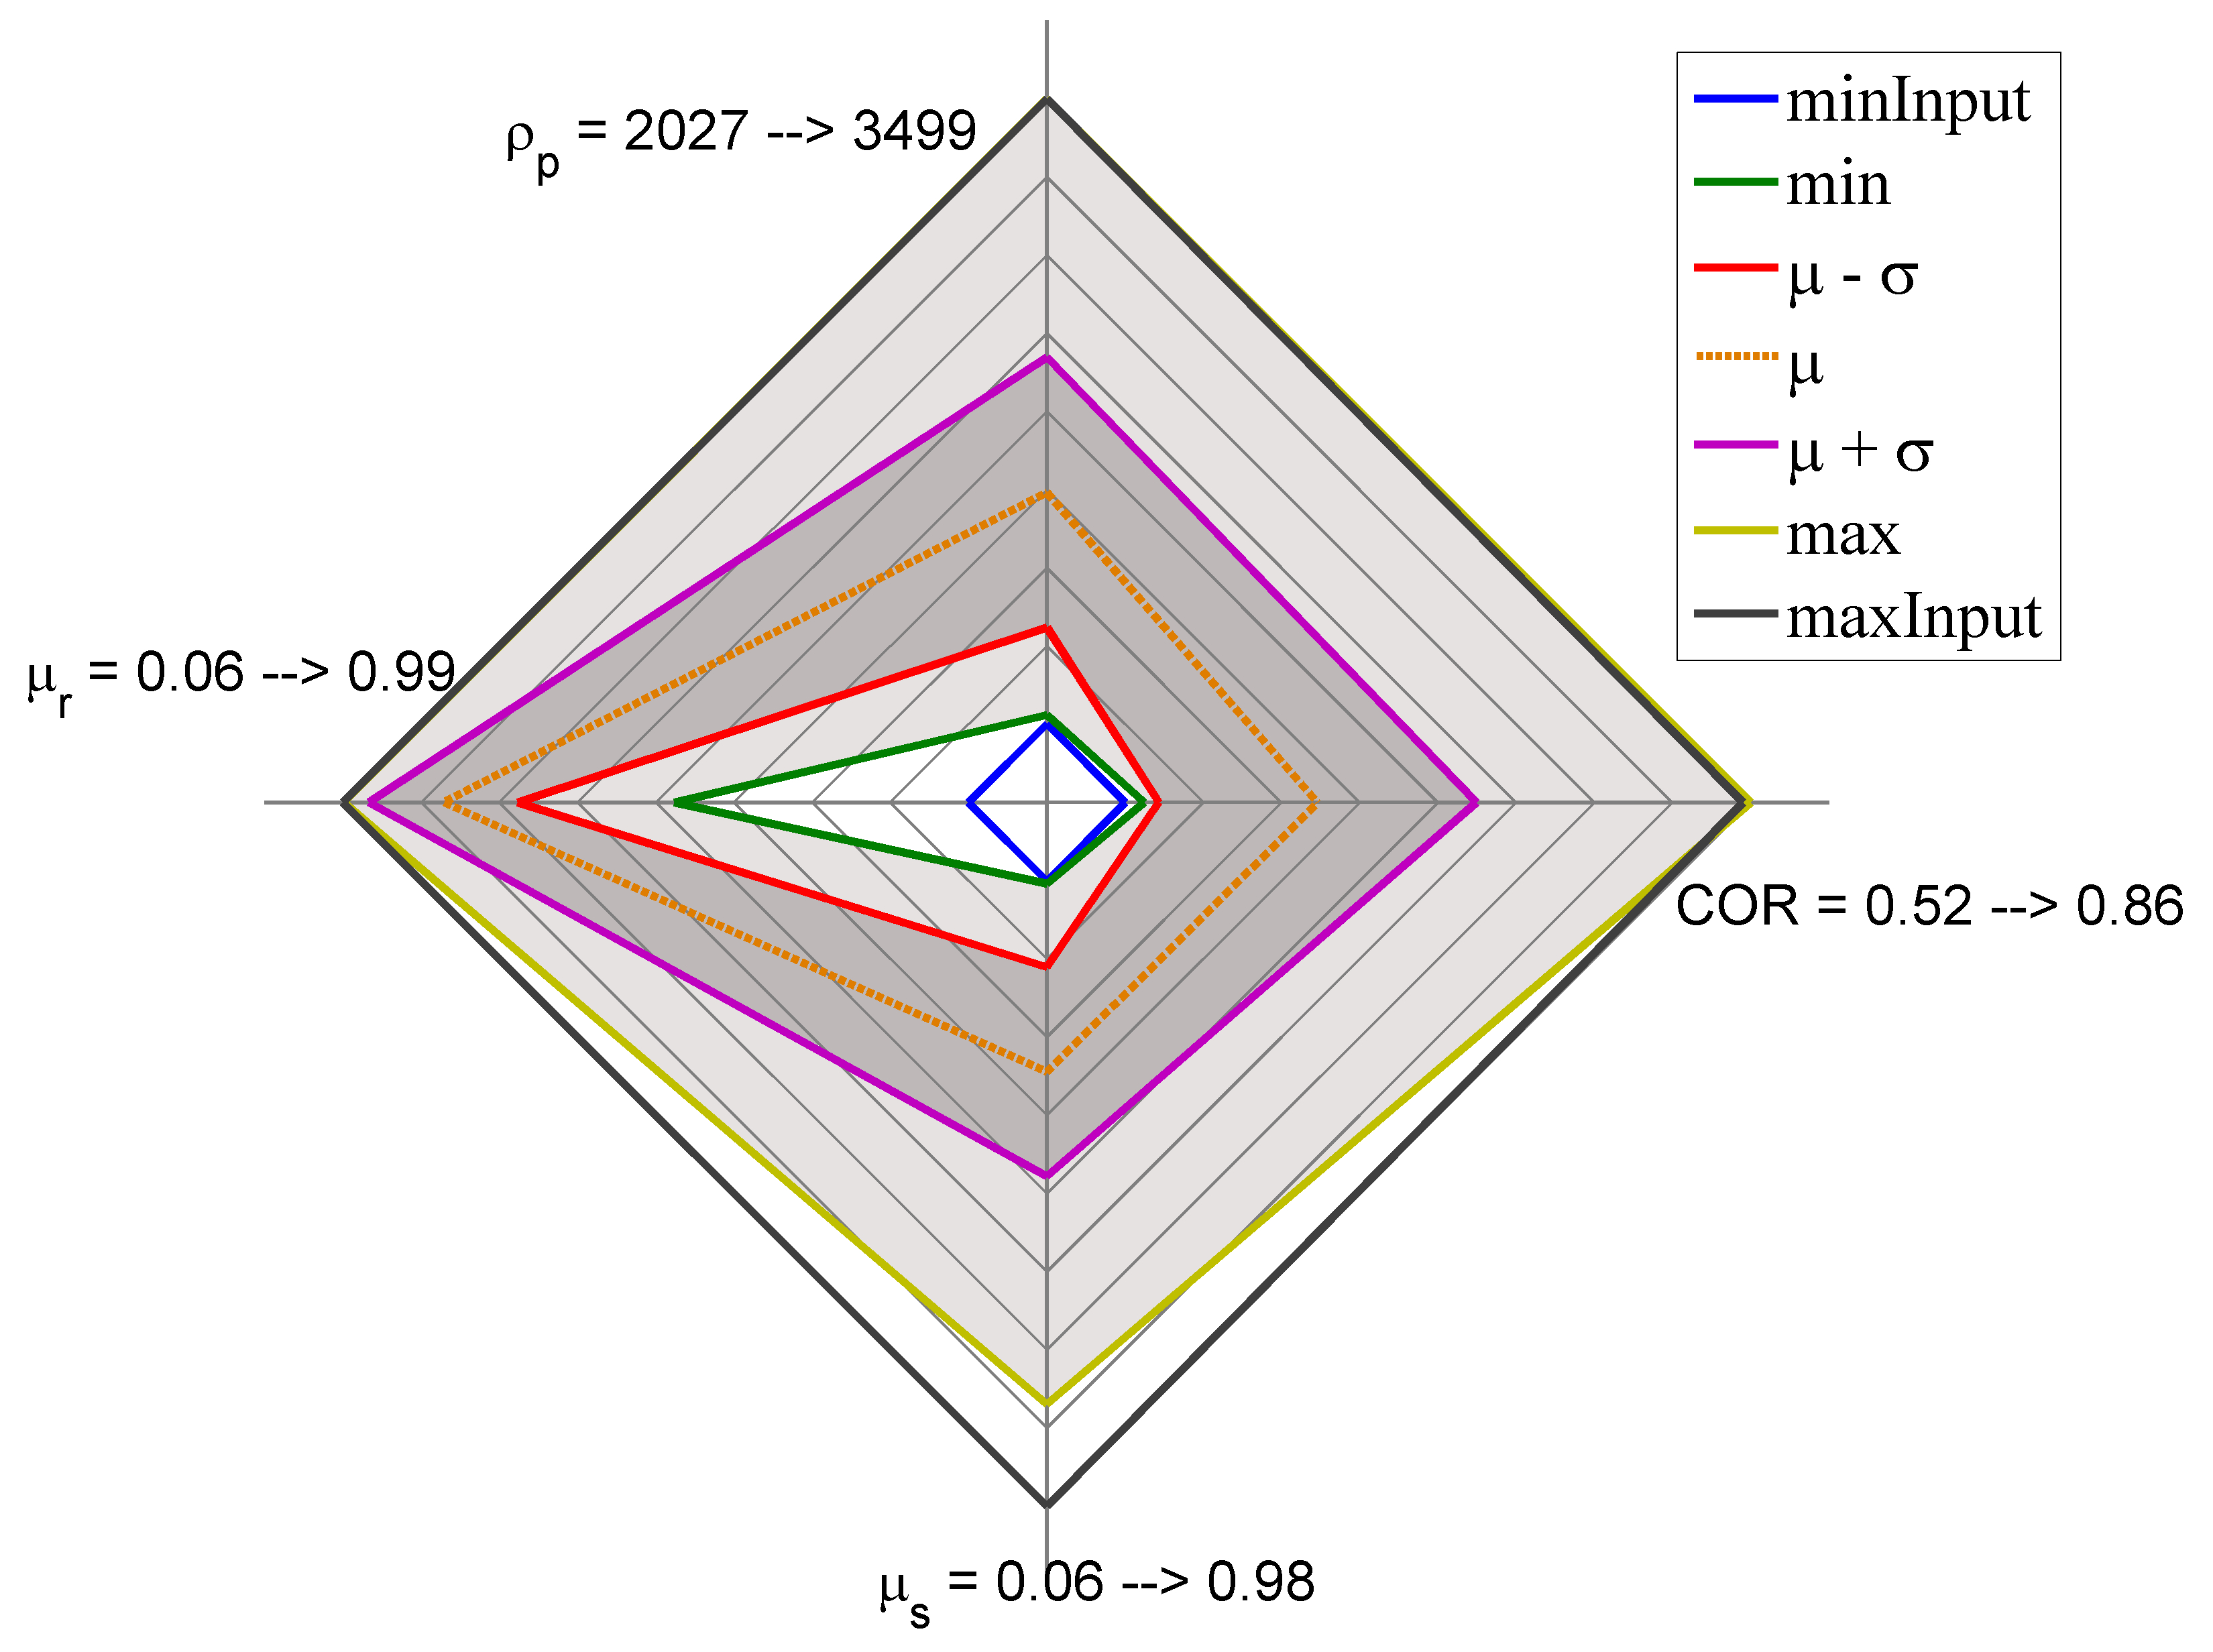
\includegraphics[width=\textwidth]{images/original/31radarpirker1aor}
        \caption{Radar P1 AOR}
        \label{fig:31radarpirker1aor} 
    \end{subfigure}
    \begin{subfigure}[b]{0.48\columnwidth}
        \includegraphics[width=\textwidth]{images/original/32cloudpirker1aor}
        \caption{Cloud P1 AOR}
        \label{fig:32cloudpirker1aor} 
    \end{subfigure}\\
        \begin{subfigure}[b]{0.48\columnwidth}
        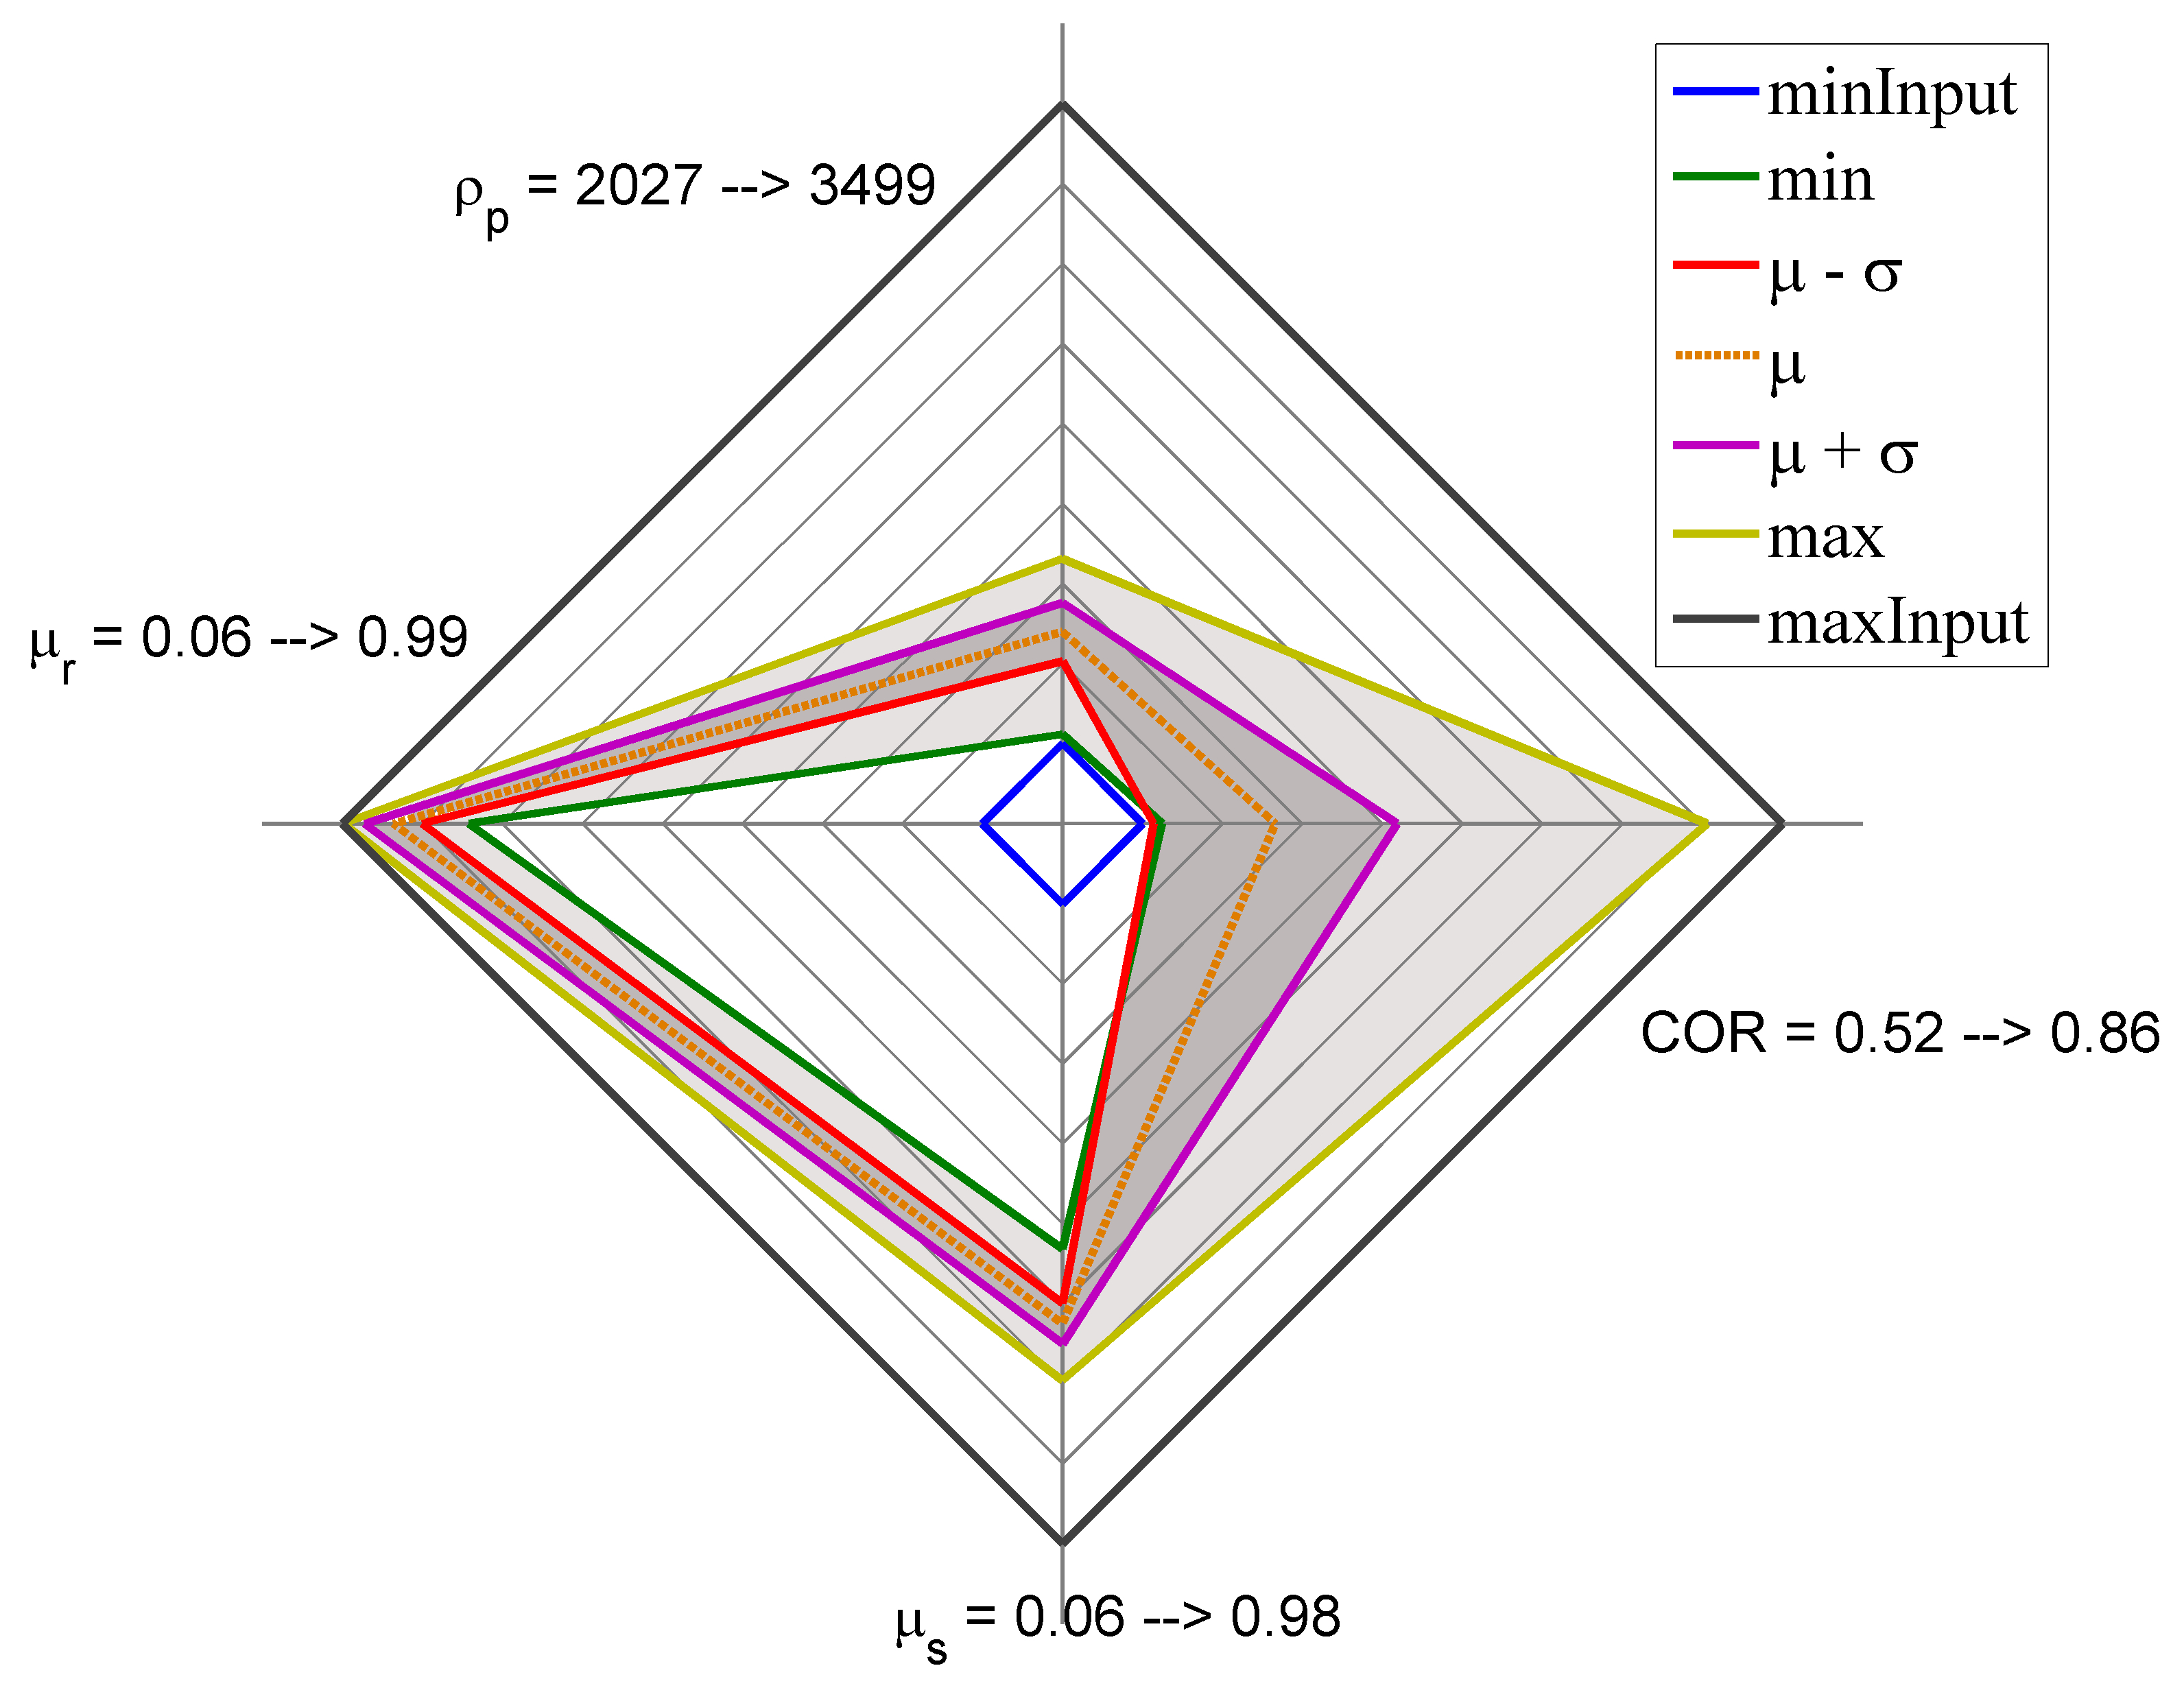
\includegraphics[width=\textwidth]{images/original/33radarpirker1schulze10070aor}
        \caption{Radar P1 Schulze 10070 & AOR}
        \label{fig:33radarpirker1schulze10070aor} 
    \end{subfigure}
    \begin{subfigure}[b]{0.48\columnwidth}
        \includegraphics[width=\textwidth]{images/original/34cloudpirker1schulze10070aor}
        \caption{Cloud P1 Schulze 10070 & AOR}
        \label{fig:34cloudpirker1schulze10070aor} 
    \end{subfigure}
    \caption{AOR and merge results.}
    \label{fig:35schulze10070aorradarandcloud}
\end{figure}
We then processed the random combinations with the $AOR$ $NN$. In Fig.
\ref{fig:31radarpirker1aor} the radar plot realized with the same criteria as
before can be seen.
In accordance with the theory (Wensrich and Katterfeld \cite{RefWorks:87}), in a simulation dominated
by the particles rolling the coefficient of rolling friction has the maximum influence. 
Further, in the cloud plot in Fig. \ref{fig:32cloudpirker1aor}
we could see that there are valid combinations also with slight $\mu_s$. \\
Finally, we extracted from the $TC1$ values the $AOR$ $NN$ behaviour
and compared it with the experimental one.
As can be seen in the radar plot in Fig.
\ref{fig:33radarpirker1schulze10070aor}, the confidence range is meager, indicating that all the parameters but the $COR$ 
had an important role and the reliability of these parameters combinations to represent the bulk behaviour. 
Also in the cloud plot in Fig. \ref{fig:34cloudpirker1schulze10070aor} we
observed a condensed distribution of valid parameters.
From the initial 6250000 combinations, only 3884 of them were valid (0.0621 \%),
see table \ref{tab:13DEMvalidvalues}.
\begin{figure}%[!h] 
\centering 
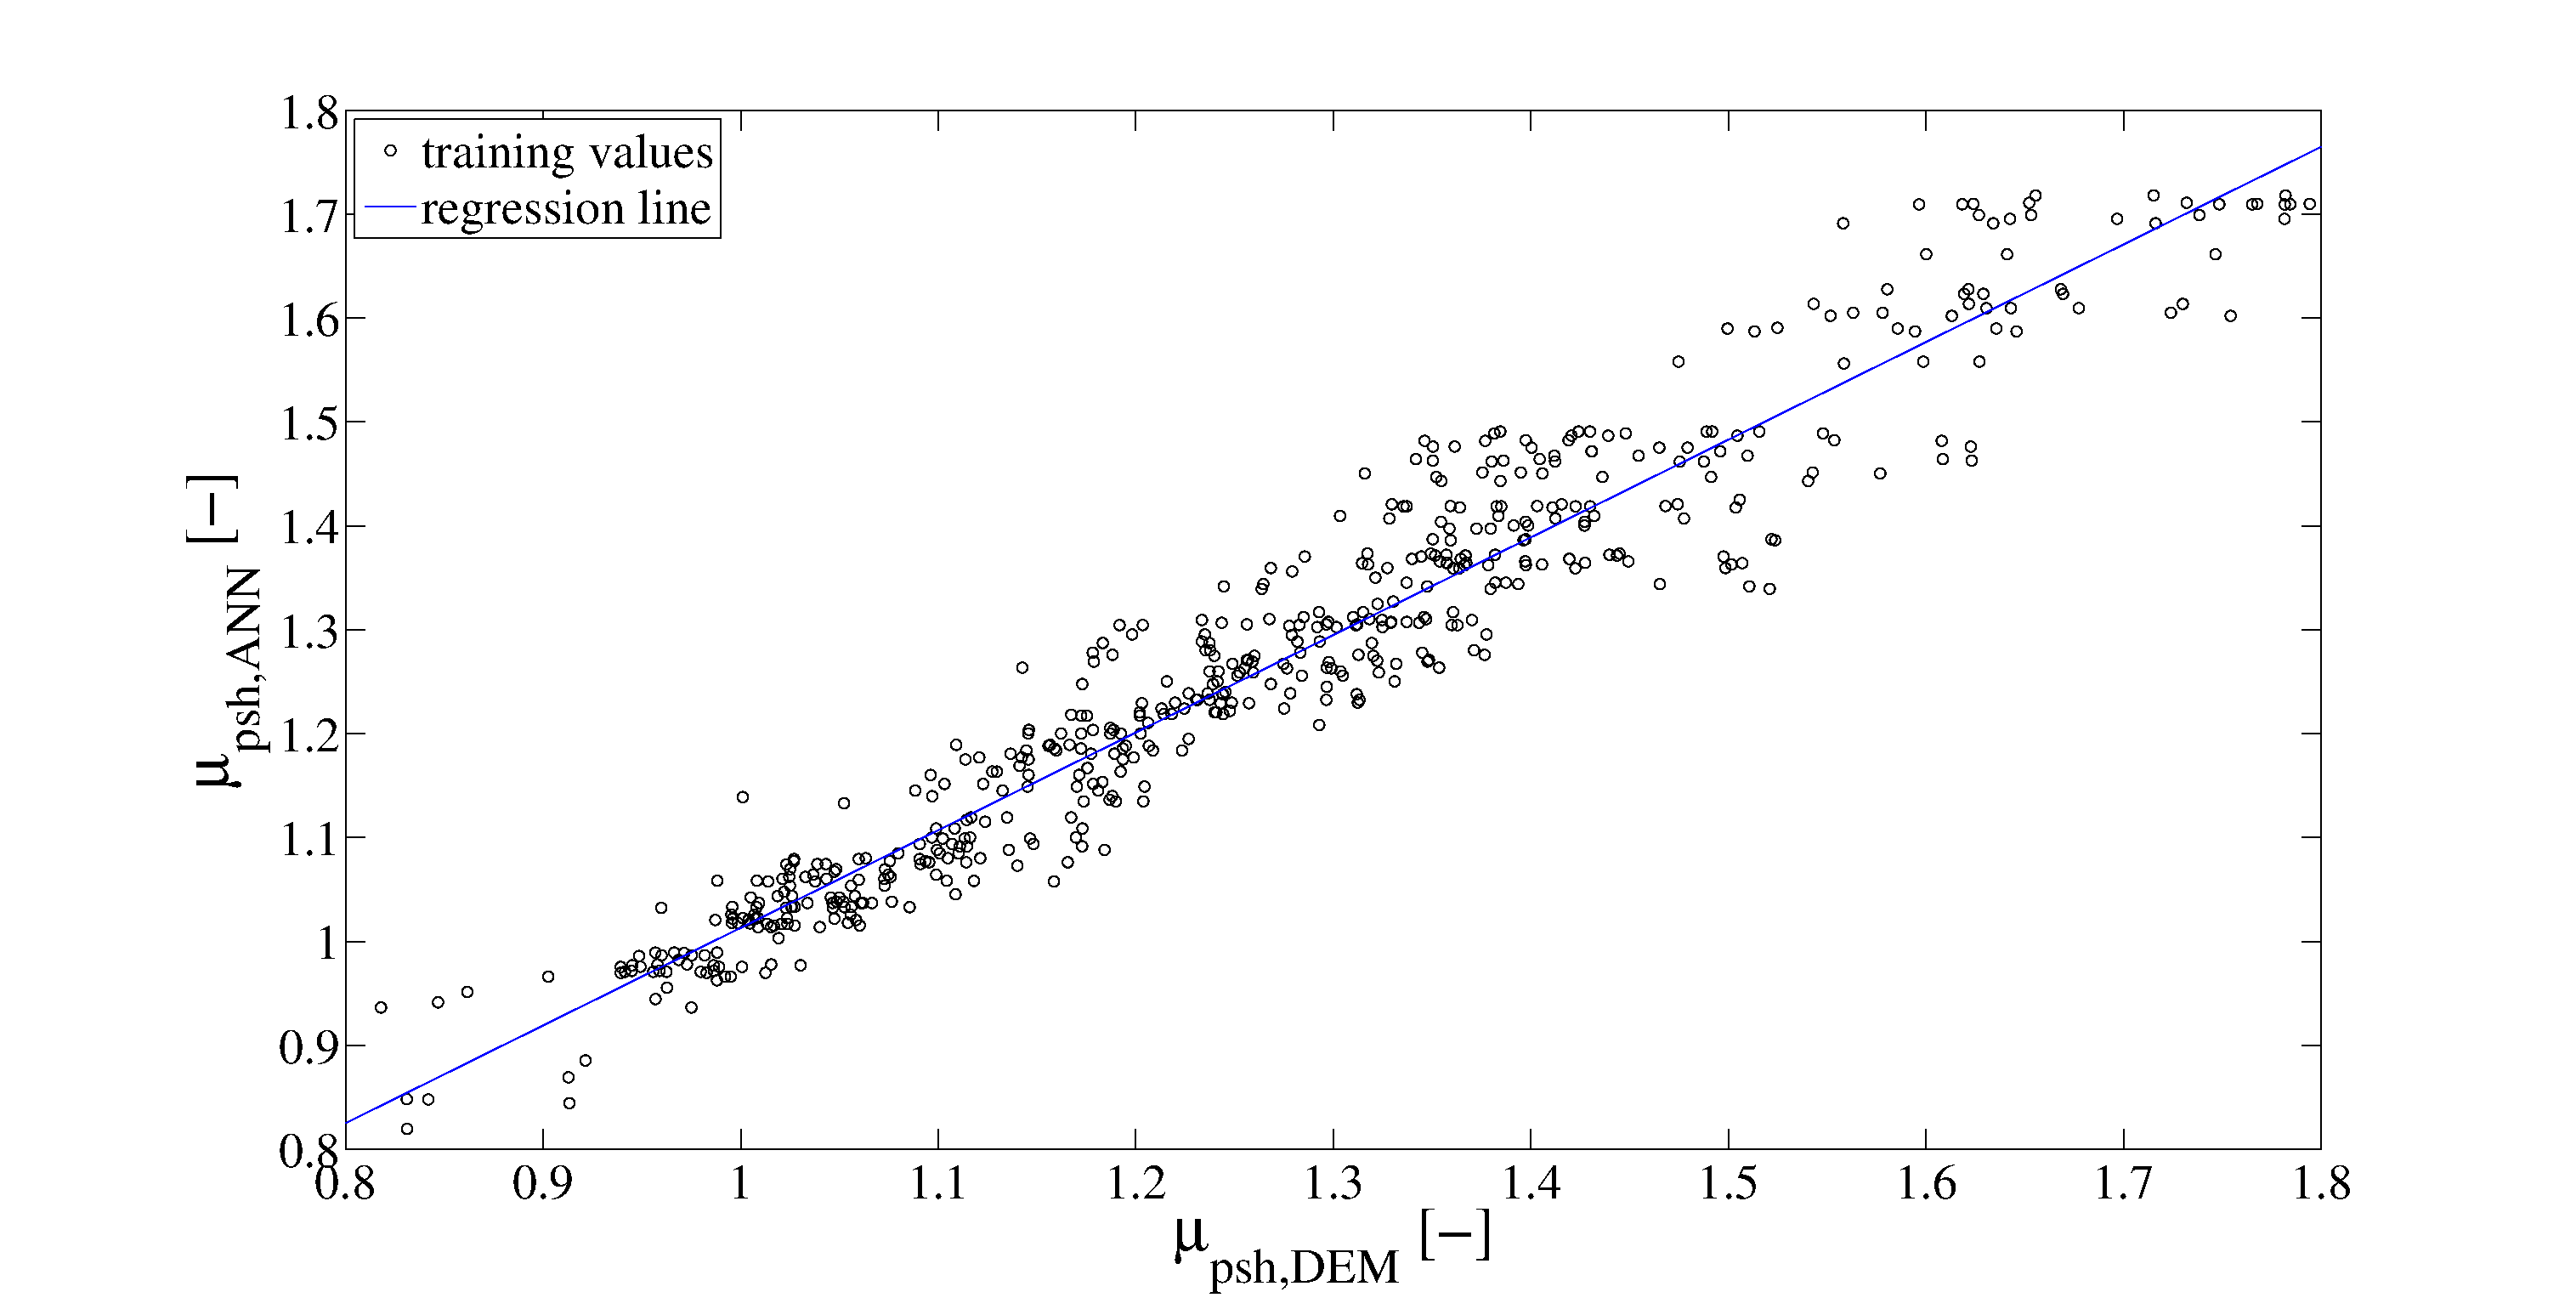
\includegraphics[width=.96\columnwidth]{images/22regression.eps}
%[width=.96\textwidth]
\caption[Comparison between prediction of the trained ANN and full DEM
simulation]{Comparison between prediction of the trained Artificial Neural
Network ($ANN$) and 546 
\wrong{write down all the simulations performed at the end.}
full DEM simulations of the coefficient of pre-shear
($\mu_{psh}$).}
\label{fig:22regression} 
\end{figure}
\begin{table}[h]
\centering
\scalebox{1.0}{
\begin{tabular}{c|cccccccc}
\hline
          & $\mu_s$ & $\mu_r$ & $COR$ & $\rho_p$ & $\mu_{sh}$ & $\mu_{psh}$ & $\rho_{b}$ & $AOR$ \\
          \hline
    $\mu_s$ & 100.00 & 0.55  & 0.04  & 0.00  & 3.84  & 87.26 & 8.39  & 49.48 \\
    $\mu_r$ & 0.55  & 100.00 & 0.15  & 0.00  & 58.92 & 33.70 & 3.10  & 60.20 \\
    $COR$ & 0.04  & 0.15  & 100.00 & 0.00  & 15.52 & 0.57  & 1.71  & 0.00 \\
    $\rho_p$ & 0.00  & 0.00  & 0.00  & 100.00 & 4.98  & 5.71  & 99.00 & 0.00 \\
    $\mu_{sh}$ & 3.84  & 58.92 & 15.52 & 4.98  & 100.00 & 26.03 & 9.52  & 0.00 \\
    $\mu_{psh}$ & \textbf{87.26} & 33.70 & 0.57  & 5.71  & 26.03 & 100.00 & 4.33 
    & 0.00
    \\
    $\rho_{b}$ & 8.39  & 3.10  & 1.71  & \textbf{99.00} & 9.52  & 4.33  & 100.00
    & 0.00 \\
    $AOR$ & 49.48 & \textbf{60.20} & 0.00  & 0.00  & 0.00  & 0.00  & 0.00  &
    100.00 \\
    
\hline
\end{tabular}}
\caption{Values of linear relationship between considered variables multiplied
for 100}
\label{tab:06inputRelationshipTable}
\end{table}
\begin{table}[h]
\centering
\begin{tabular}{llccc}
\hline

          & type  & SSC & AoR   & SSC \& AoR \\
          \hline

    $\mu_s$ & mean  & 0.831 & 0.177 & 0.664 \\
    $[-]$   & std. dev. (SD) & 0.097 & 0.095 & 0.029 \\
          & range ($R$) & 0.9   & 0.9   & 0.9 \\
          & SD / R & 0.108 & 0.106 & 0.032 \\
          \hline
    $\mu_r$ & mean  & 0.692 & 0.830 & 0.916 \\
    $[-]$   & std. dev. (SD) & 0.215 & 0.193 & 0.042 \\
          & range ($R$) & 0.9   & 0.9   & 0.9 \\
          & SD / R & 0.239 & 0.214 & 0.046 \\
          \hline
              COR   & mean  & 0.708 & 0.590 & 0.590 \\
   $ [-]$   & std. dev. (SD) & 0.104 & 0.073 & 0.065 \\
          & range ($R$) & 0.4   & 0.4   & 0.4 \\
          & SD / R & 0.259 & 0.183 & 0.161 \\
          \hline
    $\rho_p$ & mean  & 2245.7 & 3192.8 & 2283.9 \\
    $[kg/m3]$ & std. dev. (SD) & 80.5  & 277.4 & 67.1 \\
          & range ($R$) & 1500  & 1500  & 1500 \\
          & SD / R & 0.054 & 0.185 & 0.045 \\
          \hline
    valid & number & 290203 & 816552 & 3884 \\
    combinations & [$\%$] & 4.64  & 13.06 & 0.06 \\  

\hline
\end{tabular}
\caption[DEM valid values]{DEM valid values. For each parameter we show the
valid parameters statistics in the two tests and in their intersection.
Finally, we show the number of valid parameters combinations over the total
(6250000).}
\label{tab:13DEMvalidvalues}
\end{table}
%\begin{figure}[!h] 
\centering 
\includegraphics[width=.96\textwidth]{images/original/23regressiongraph}
%[width=.96\textwidth]
\caption{Regression graph}
\label{fig:23regressiongraph} 
\end{figure}


% \begin{figure}[htp]
%     \centering
%     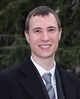
\includegraphics[width=.2\textwidth]{images/vitae/lbenvenuti}
%     \caption{OpenMP, MPI, MPI/OpenMP Hybrid runs of Box in a box testcase on 32
%     cores. The OpenMP-only run suffers from limited memory bandwidth in
%     memory-bound algorithms inside of the Modify section of the code. MPI-only has
%     low averaged runtimes for each section, but a very large Other timing, which
%     hints for a large amount of load-imbalance. Hybrid timings are a bit worse
%     on average, but because of better balancing, processes have lower wait times
%     inside of Other timing.}
% 	\label{fig:boxInBoxComparison}

%\begin{figure}[htp] \centering
    \begin{subfigure}[b]{0.48\columnwidth}
        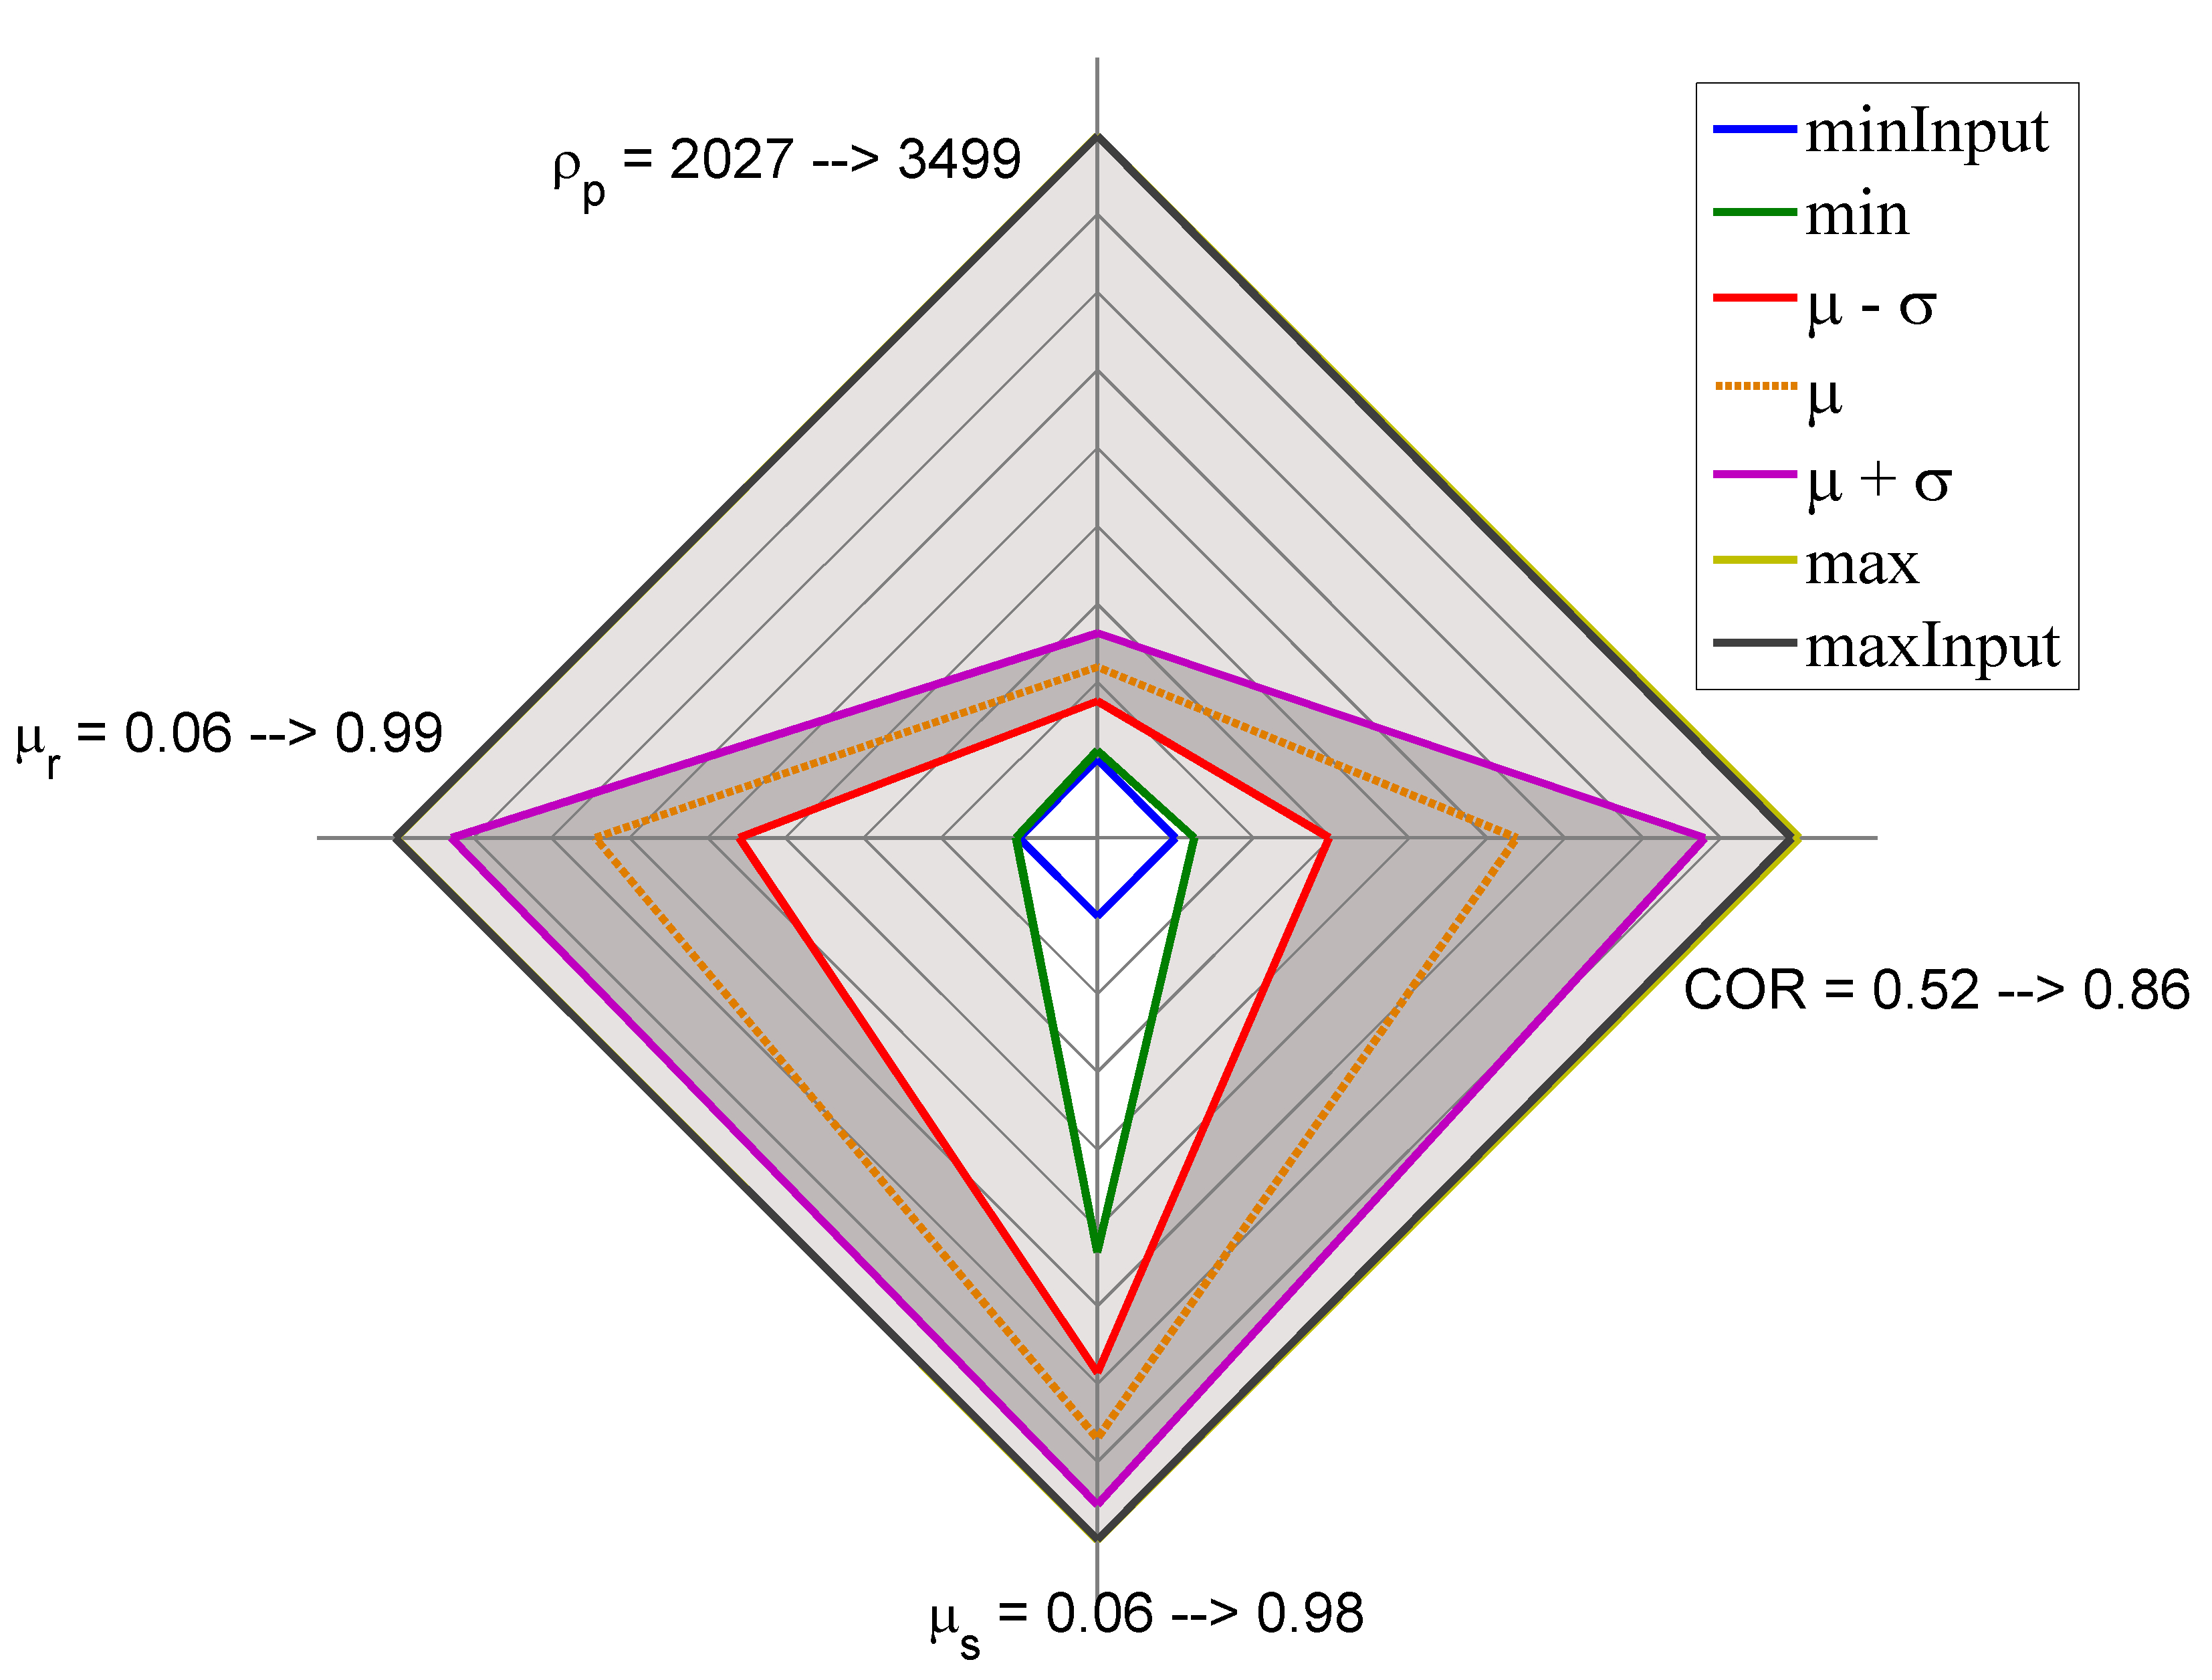
\includegraphics[width=\textwidth]{images/original/24radarpirker1schulze10070}
        \caption{Radar P1 Schulze10070}
        \label{fig:24radarpirker1schulze10070}
    \end{subfigure}
    \begin{subfigure}[b]{0.48\columnwidth}
        \includegraphics[width=\textwidth]{images/original/25cloudpirker1schulze10070}
        \caption{Cloud P1 Schulze10070}
        \label{fig:25cloudpirker1schulze10070}
    \end{subfigure}\\
        \begin{subfigure}[b]{0.48\columnwidth}
        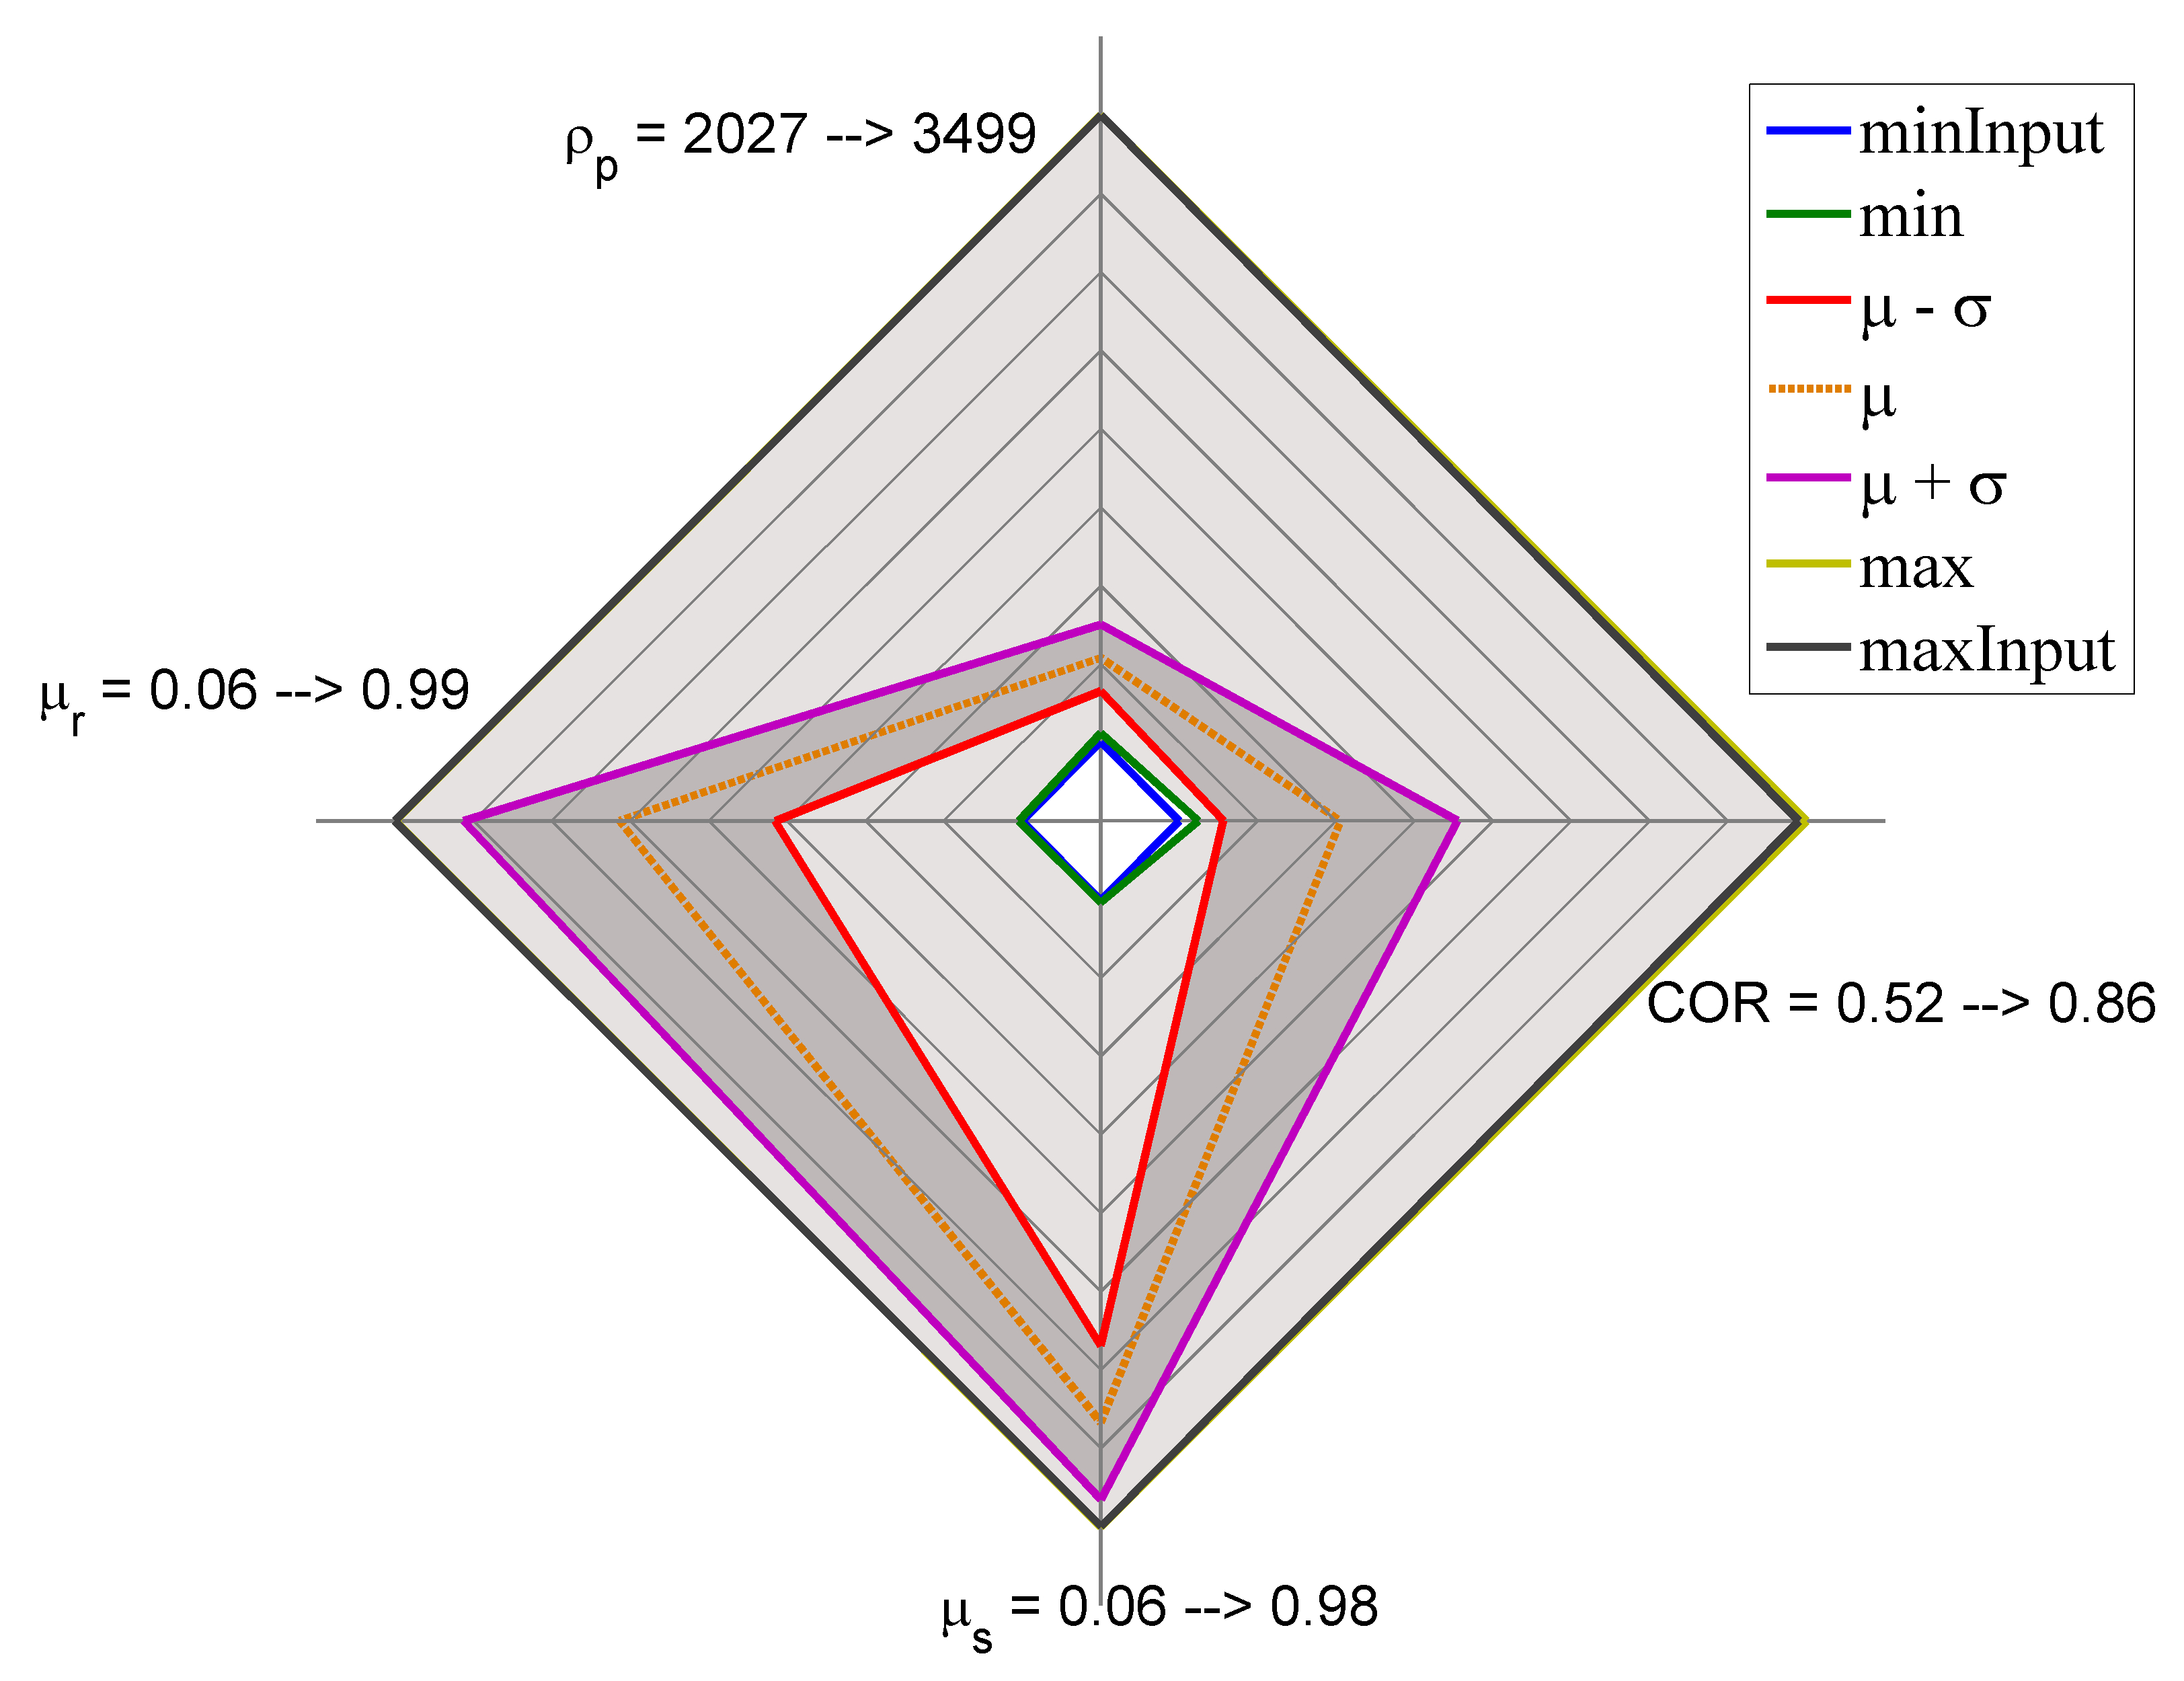
\includegraphics[width=\textwidth]{images/original/26radarpirker08schulze10070}
        \caption{Radar P08 Schulze10070}
        \label{fig:26radarpirker08schulze10070} 
    \end{subfigure}
    \begin{subfigure}[b]{0.48\columnwidth}
        \includegraphics[width=\textwidth]{images/original/27cloudpirker08schulze10070}
        \caption{Cloud P08 Schulze10070}
        \label{fig:27cloudpirker08schulze10070} 
    \end{subfigure}\\
        \begin{subfigure}[b]{0.48\columnwidth}
        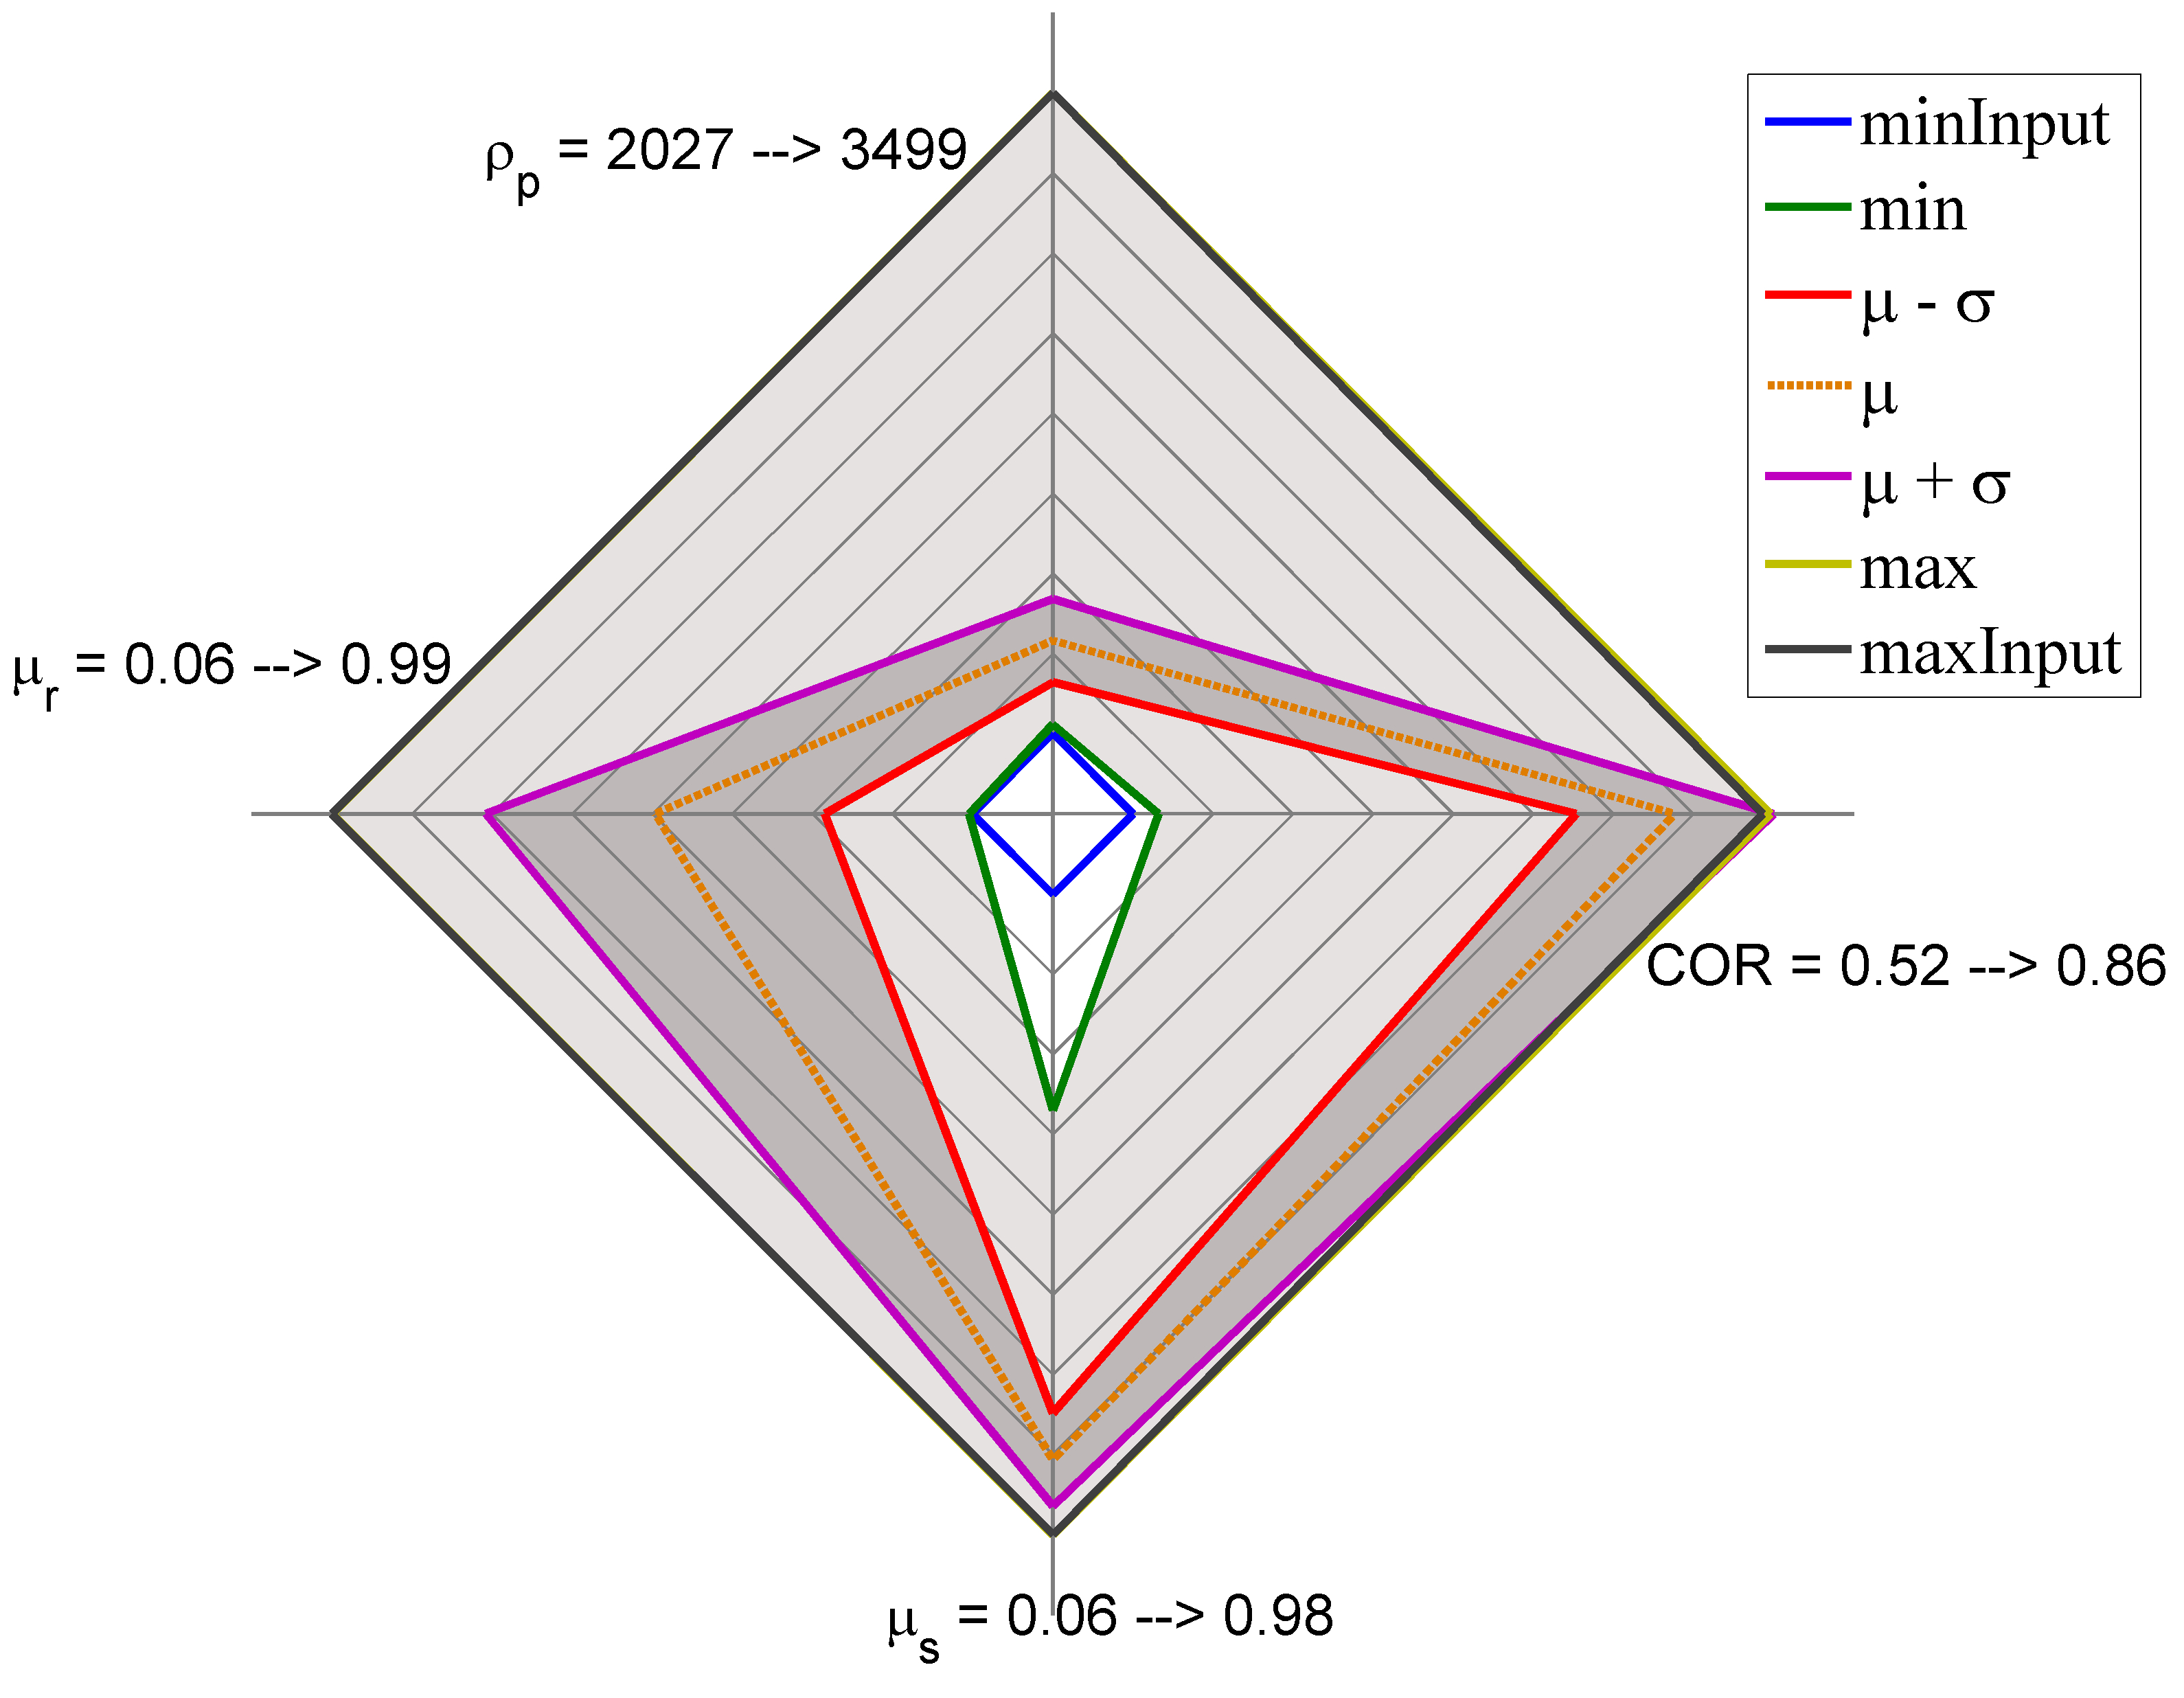
\includegraphics[width=\textwidth]{images/original/28radarpirker12schulze10070}
        \caption{Radar P12 Schulze10070}
        \label{fig:28radarpirker12schulze10070} 
    \end{subfigure}
    \begin{subfigure}[b]{0.48\columnwidth}
        \includegraphics[width=\textwidth]{images/original/30cloudpirker12schulze10070}
        \caption{Cloud P12 Schulze10070}
        \label{fig:30cloudpirker12schulze10070} 
    \end{subfigure}
    \caption{Comparison between the original experimental selection P=1 and the
    increased and decreased results.}
    \label{fig:29schulzeradarandcloud}
\end{figure}
%\begin{figure}[htp] \centering
    \begin{subfigure}[b]{0.48\columnwidth}
        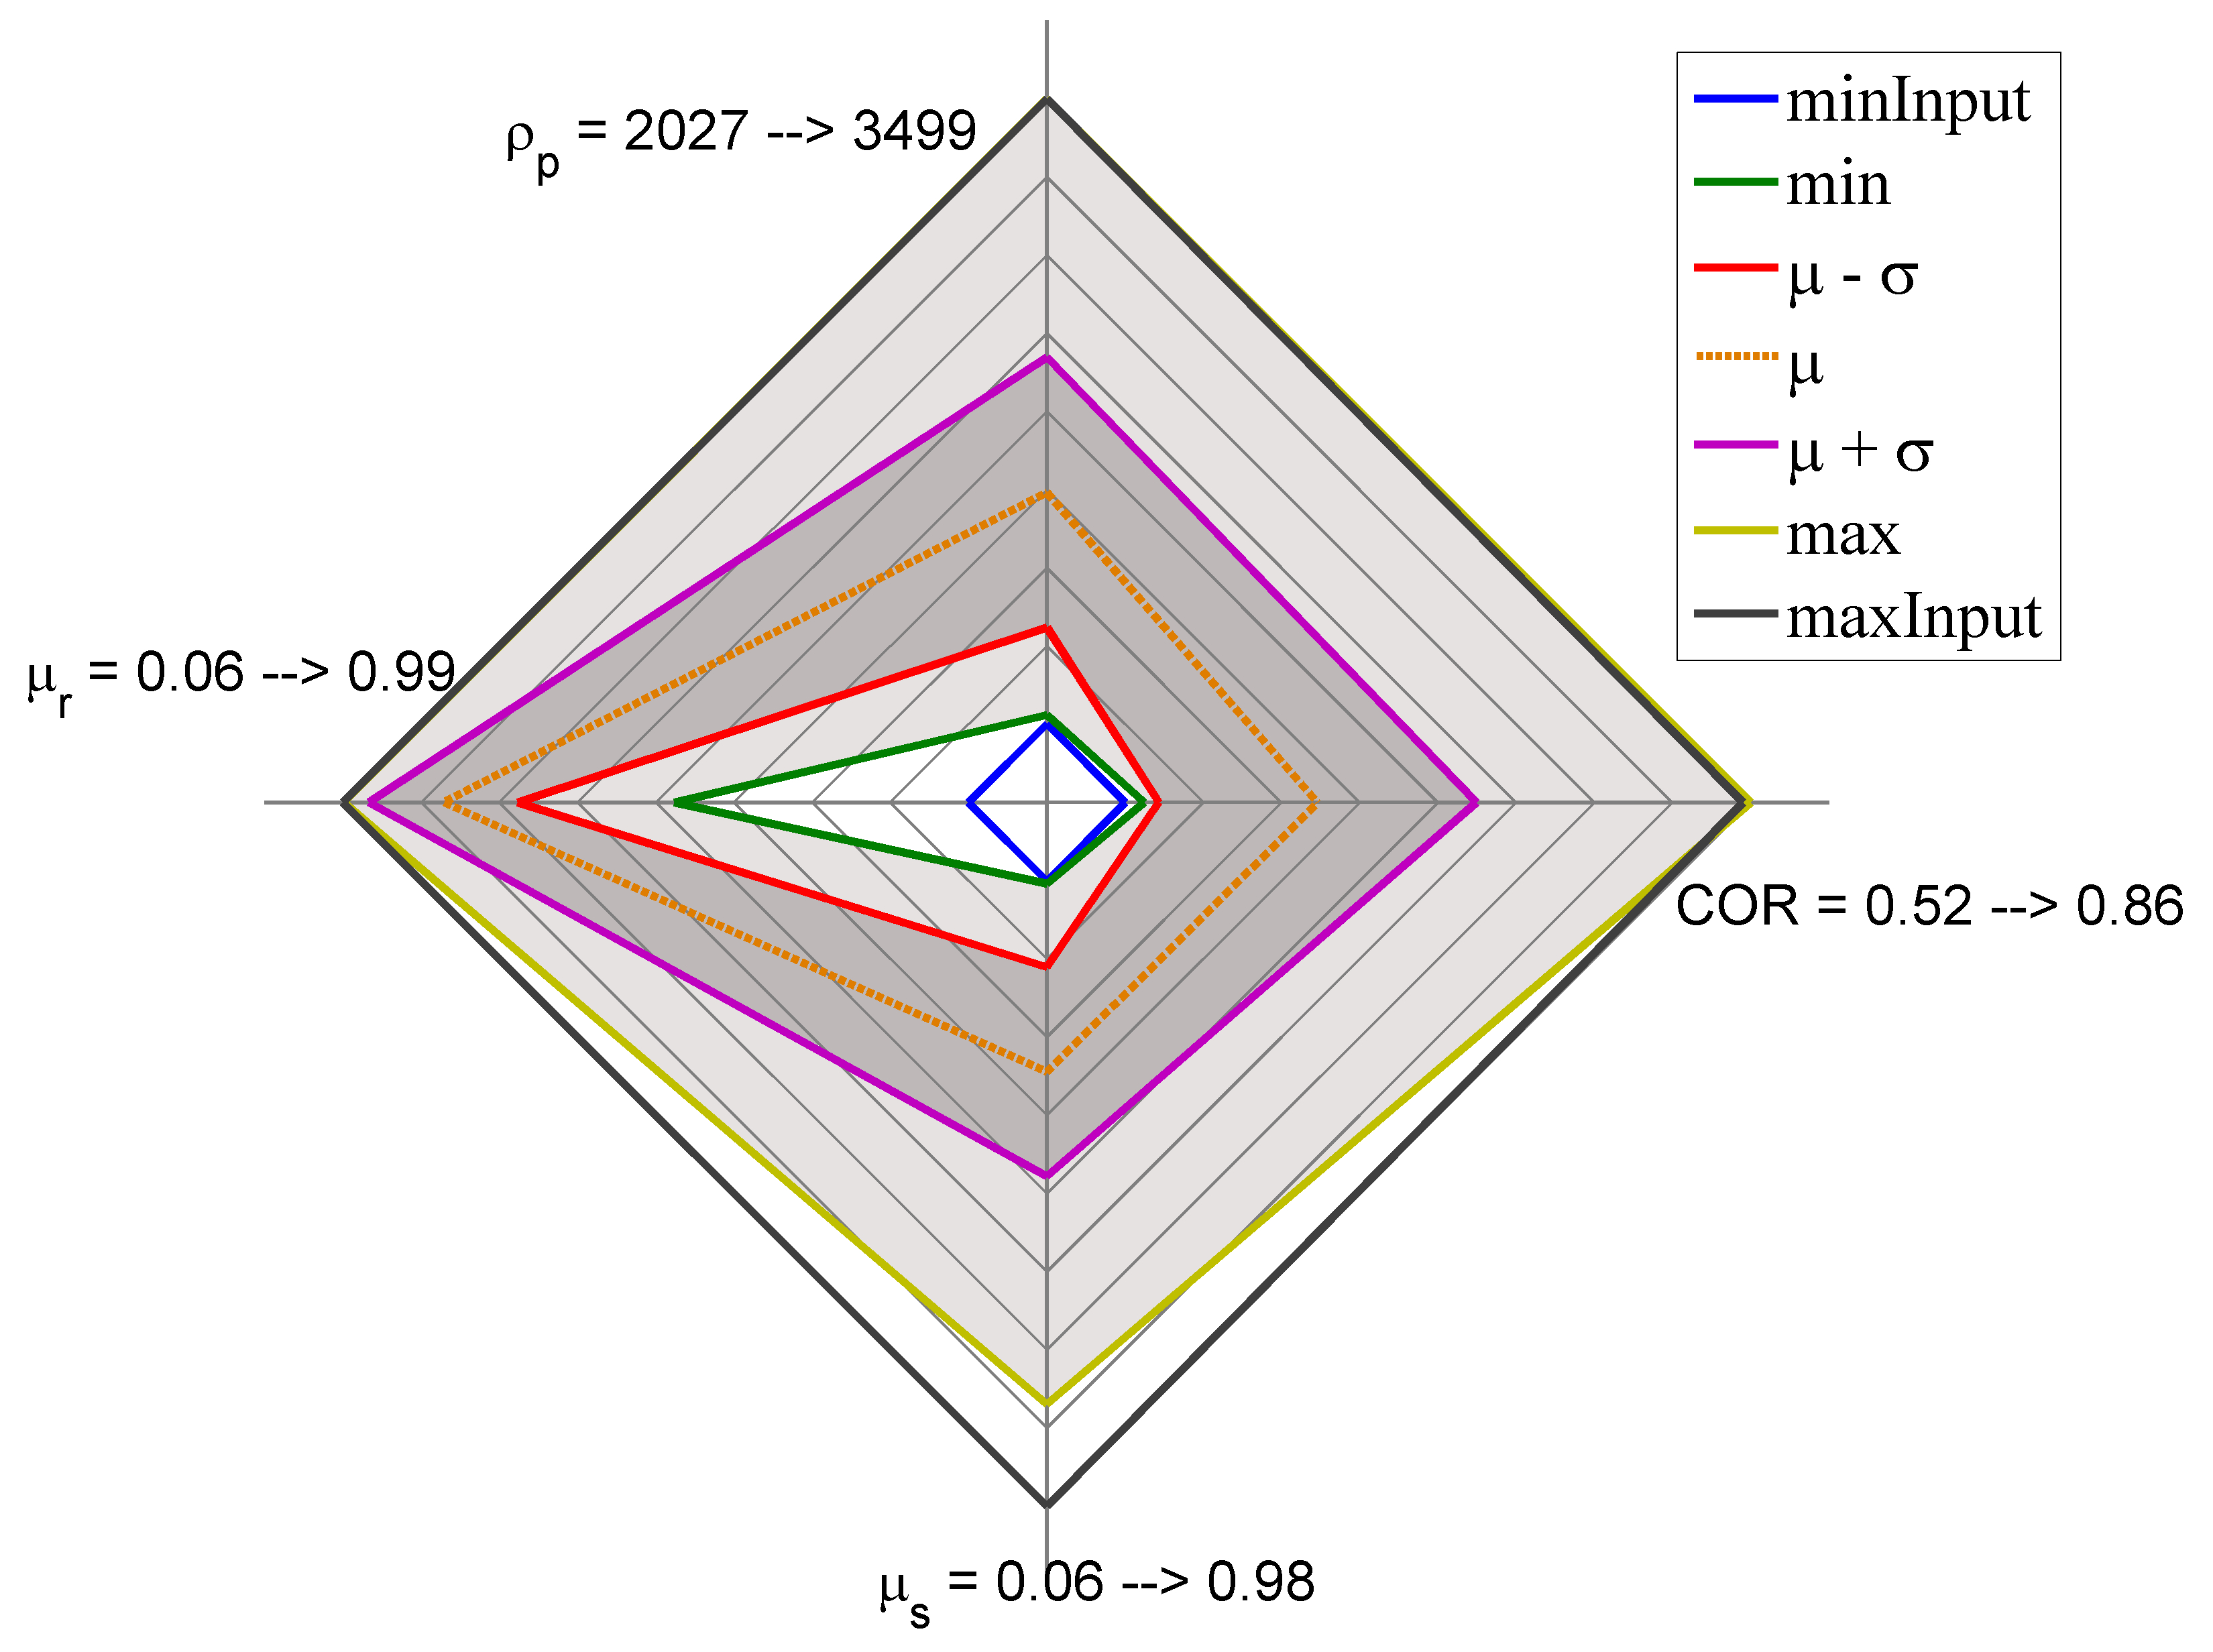
\includegraphics[width=\textwidth]{images/original/31radarpirker1aor}
        \caption{Radar P1 AOR}
        \label{fig:31radarpirker1aor} 
    \end{subfigure}
    \begin{subfigure}[b]{0.48\columnwidth}
        \includegraphics[width=\textwidth]{images/original/32cloudpirker1aor}
        \caption{Cloud P1 AOR}
        \label{fig:32cloudpirker1aor} 
    \end{subfigure}\\
        \begin{subfigure}[b]{0.48\columnwidth}
        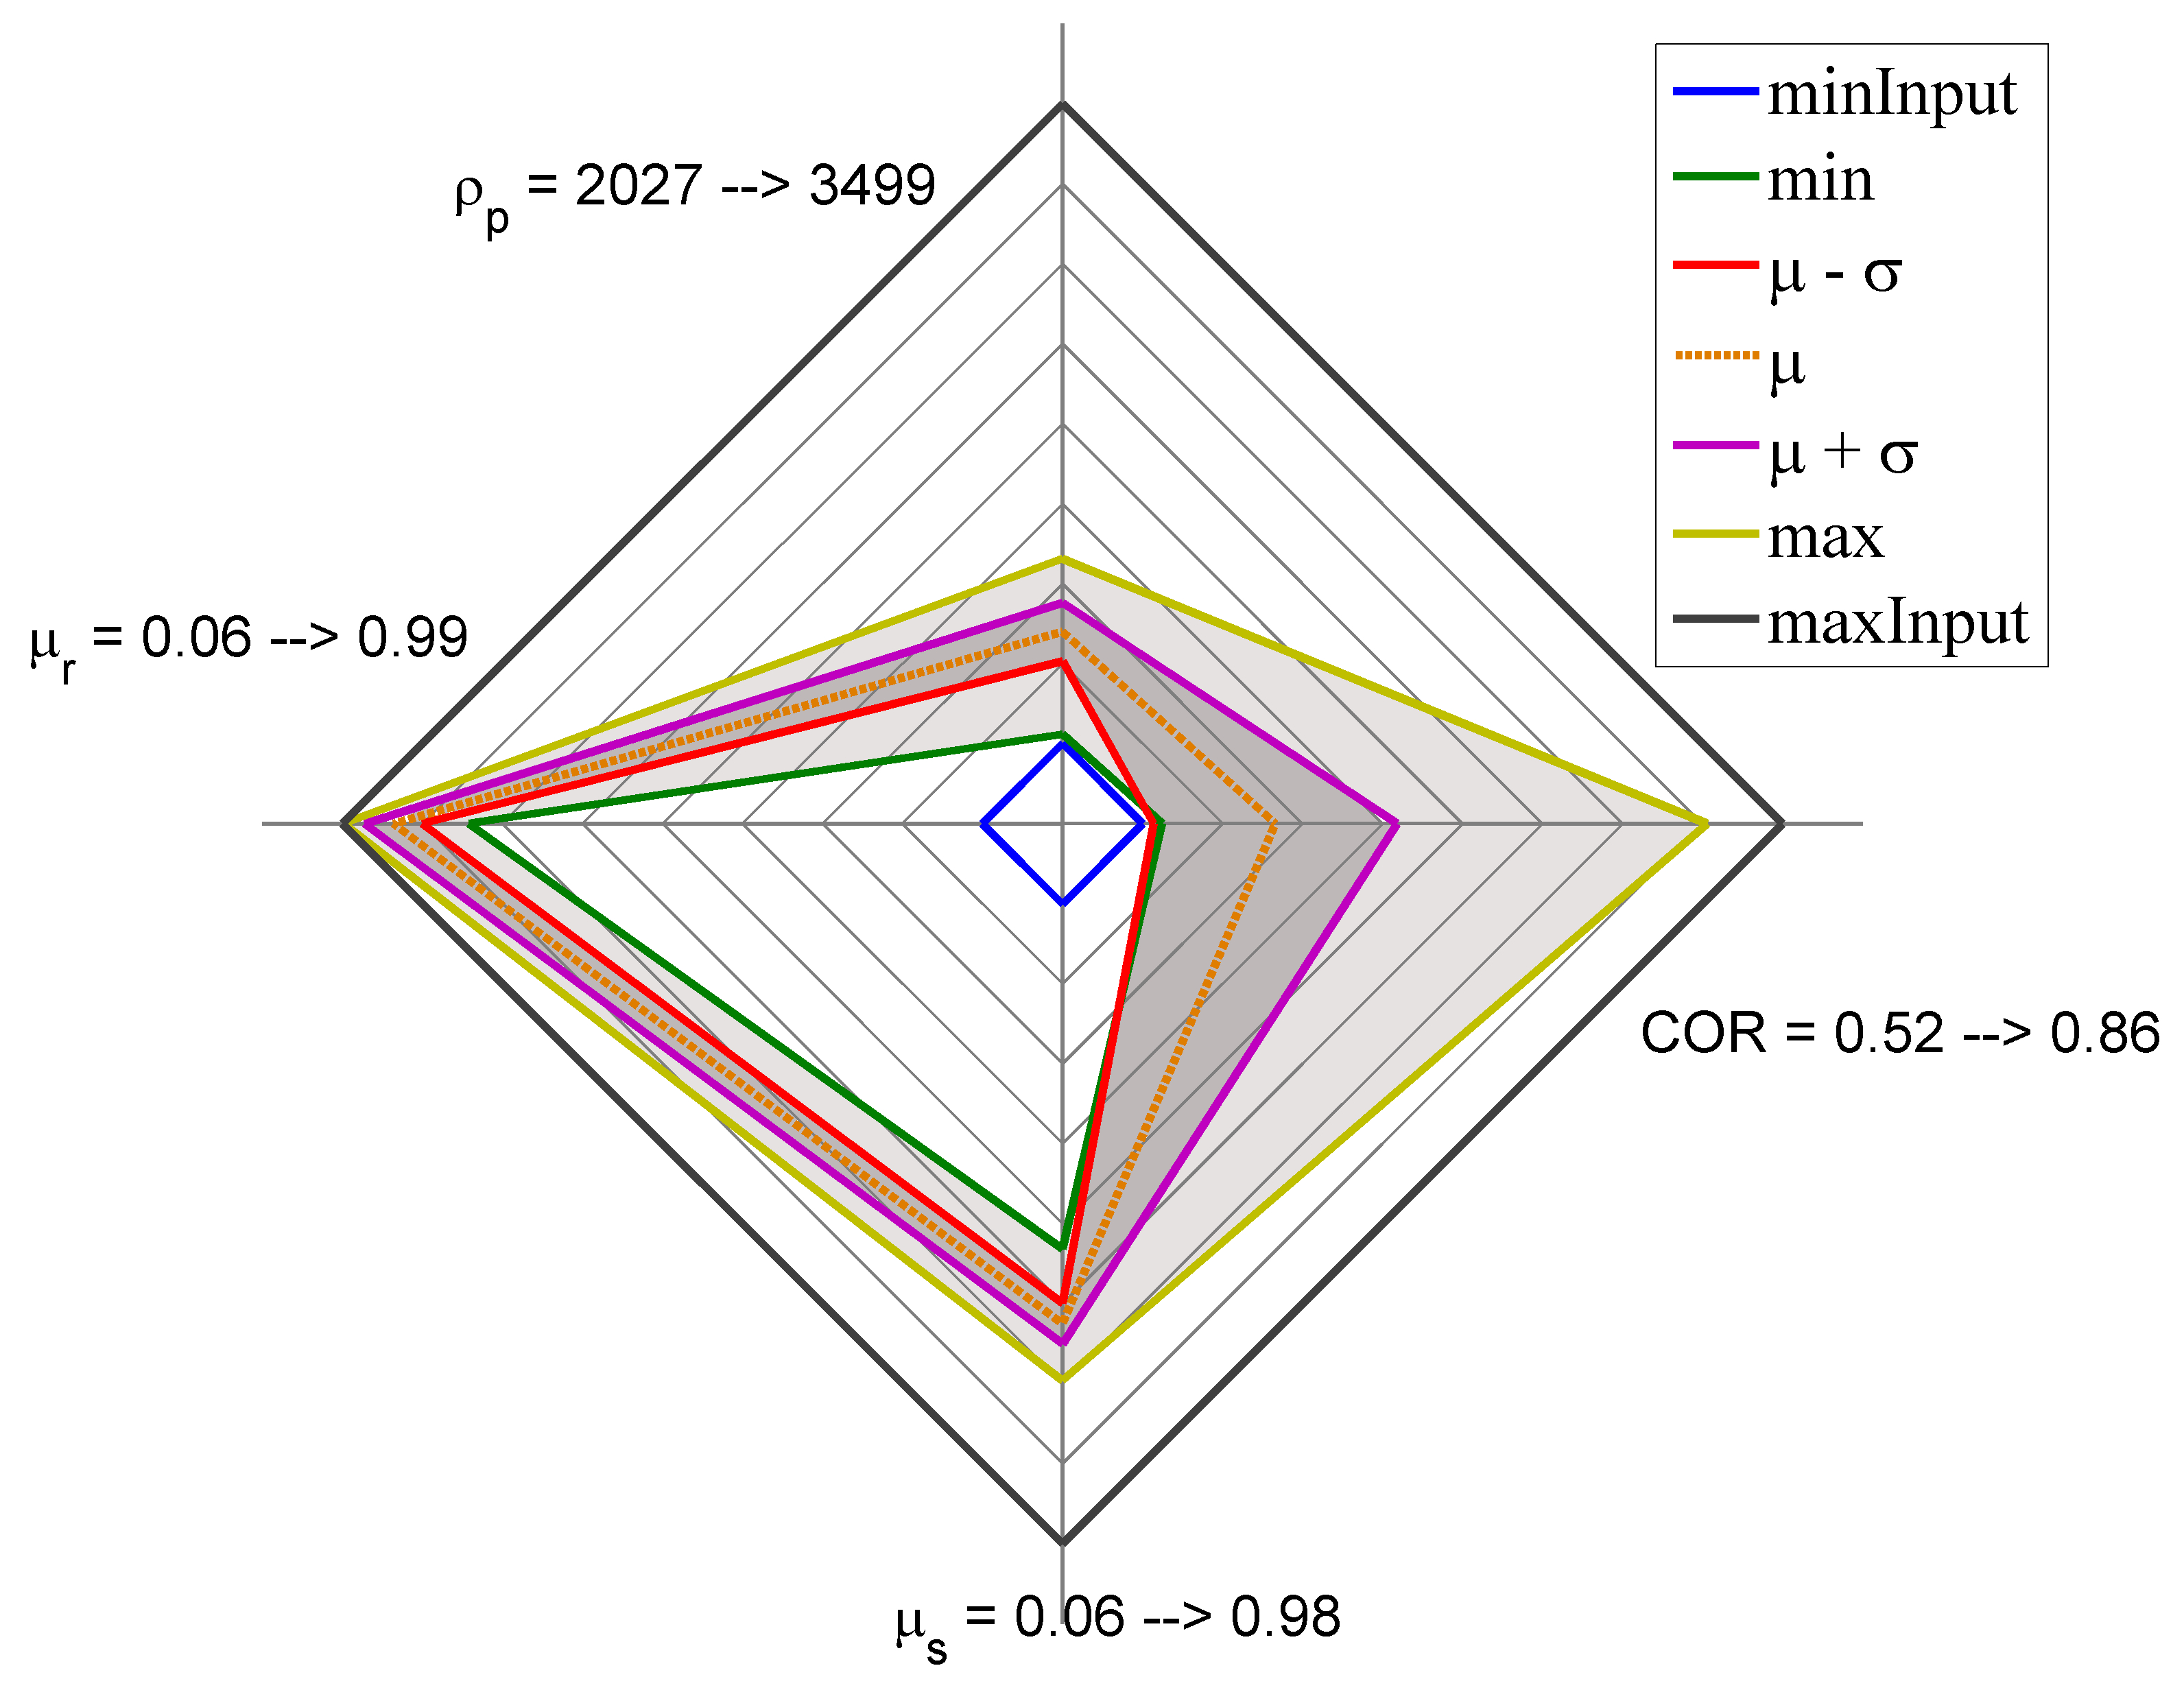
\includegraphics[width=\textwidth]{images/original/33radarpirker1schulze10070aor}
        \caption{Radar P1 Schulze 10070 & AOR}
        \label{fig:33radarpirker1schulze10070aor} 
    \end{subfigure}
    \begin{subfigure}[b]{0.48\columnwidth}
        \includegraphics[width=\textwidth]{images/original/34cloudpirker1schulze10070aor}
        \caption{Cloud P1 Schulze 10070 & AOR}
        \label{fig:34cloudpirker1schulze10070aor} 
    \end{subfigure}
    \caption{AOR and merge results.}
    \label{fig:35schulze10070aorradarandcloud}
\end{figure}
\begin{figure}[htp] \centering
    \begin{subfigure}
        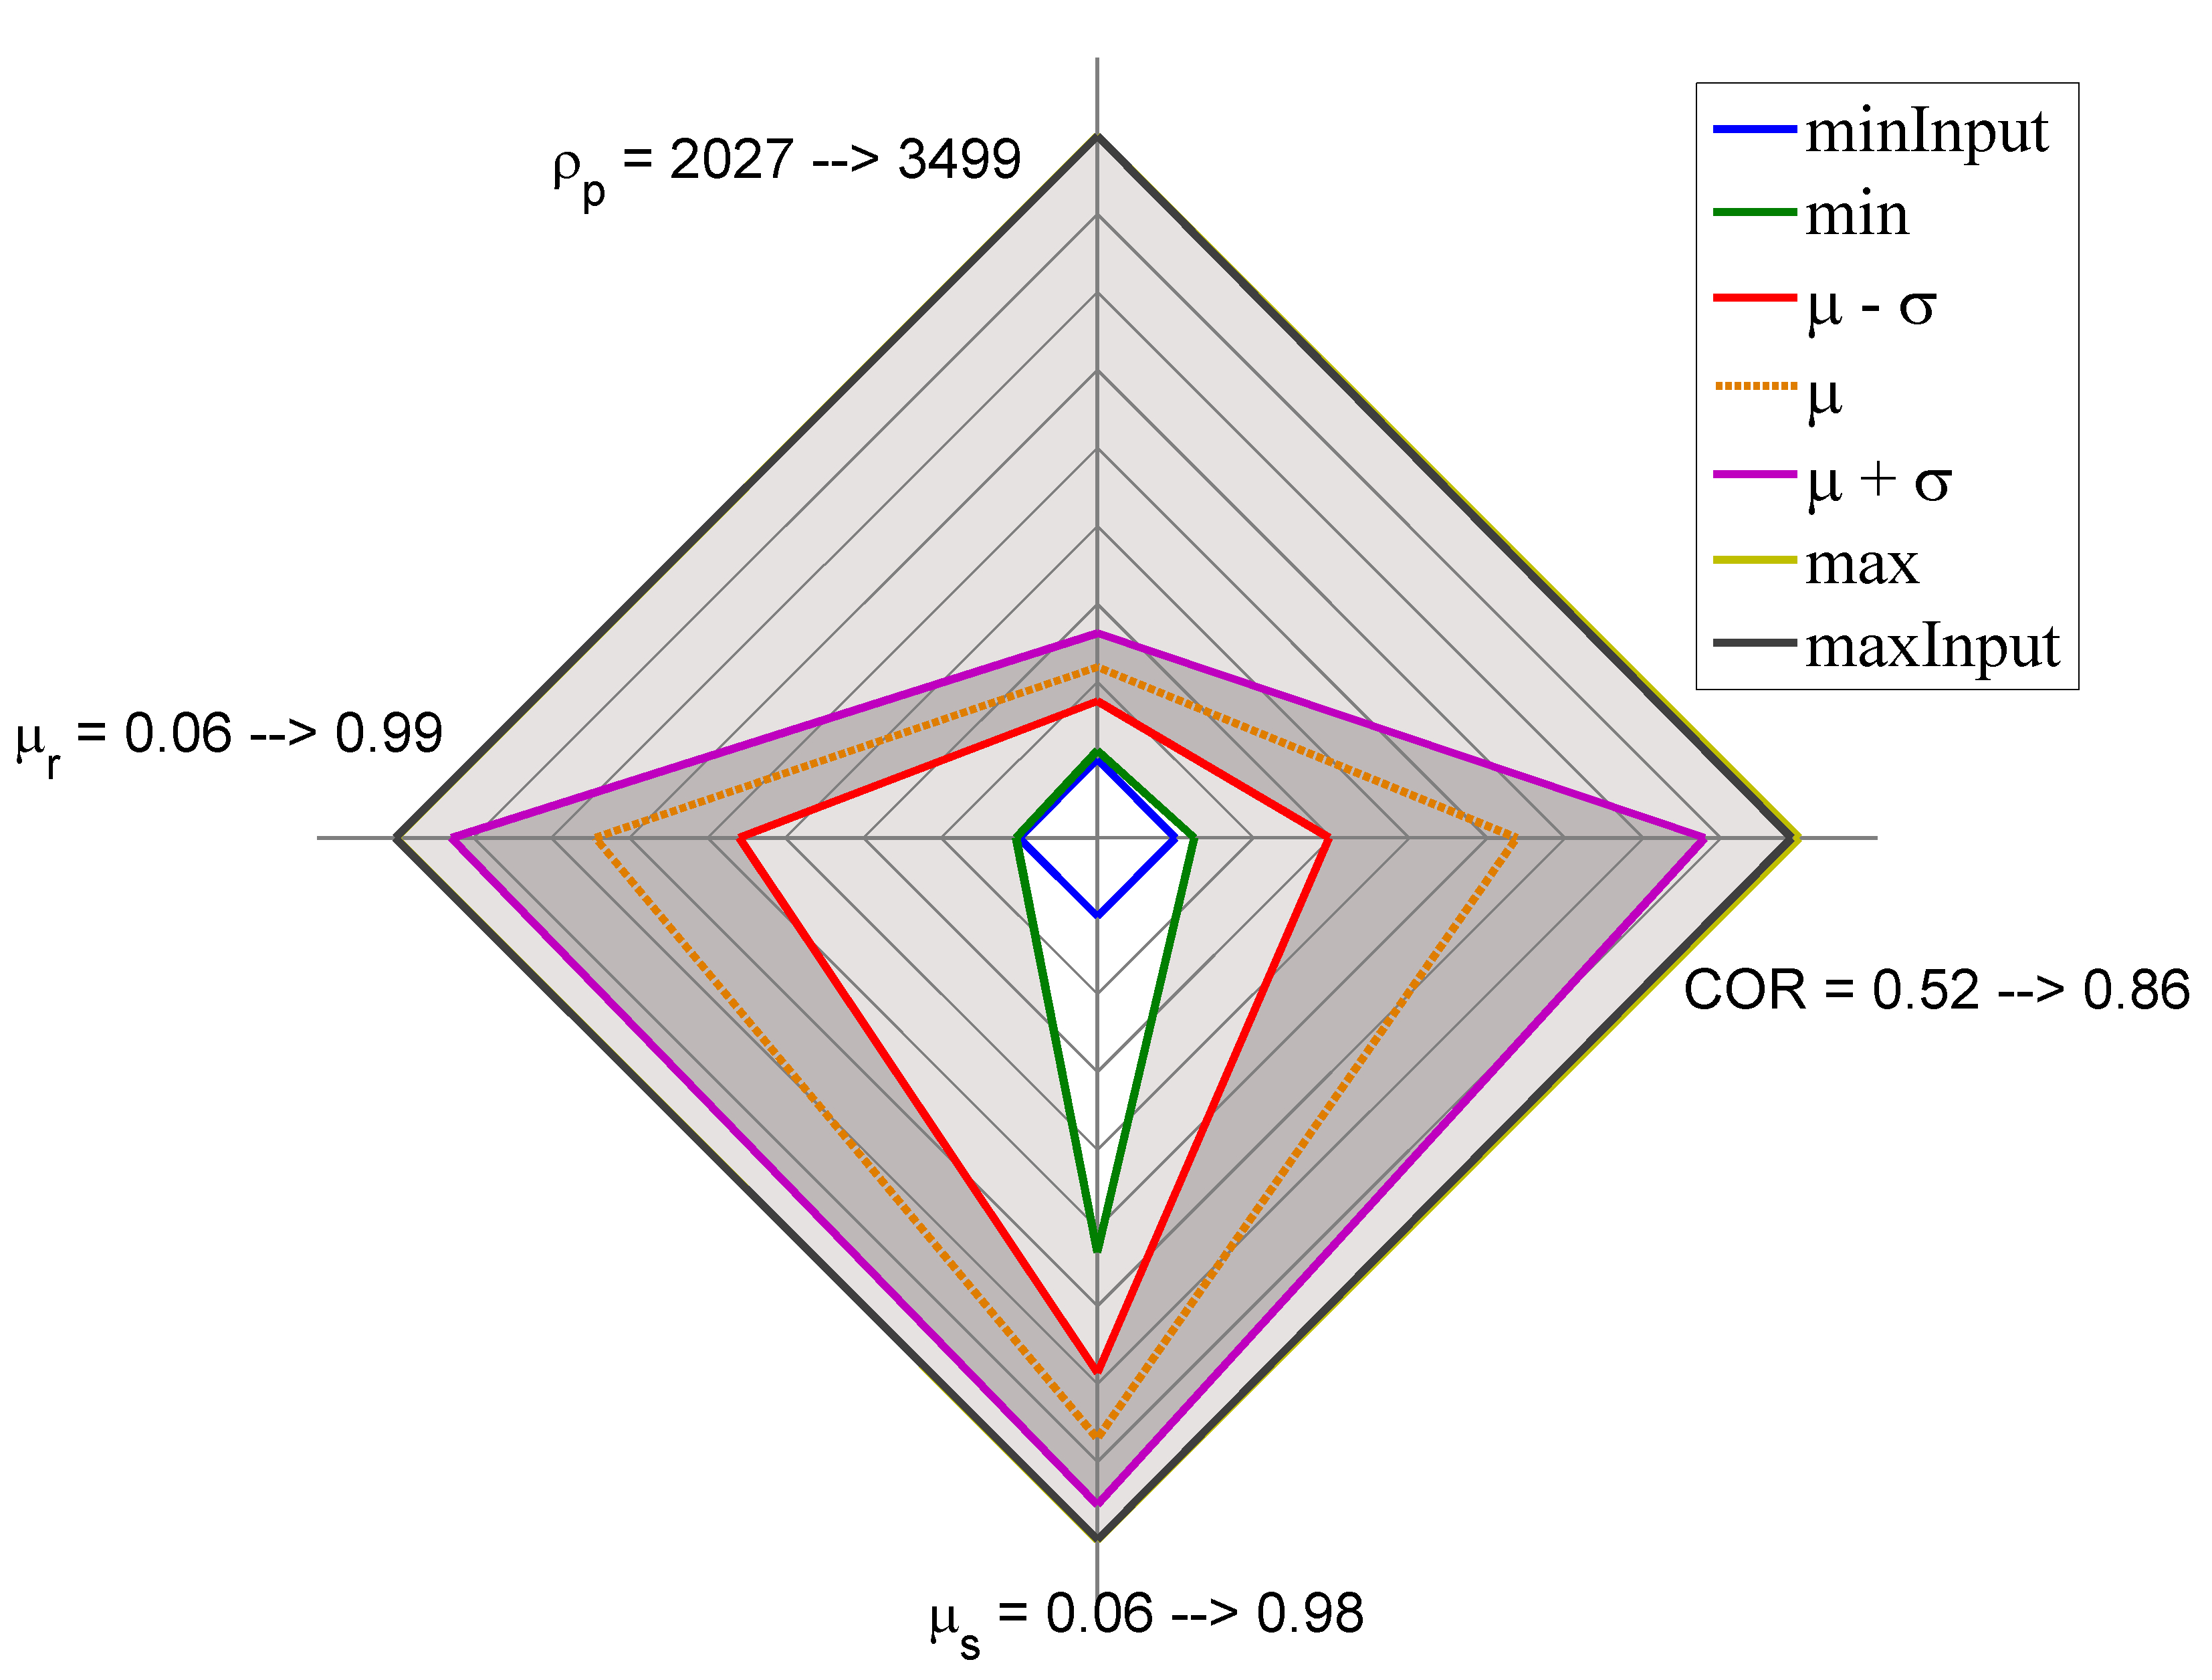
\includegraphics[width=0.5\textwidth]{images/original/24radarpirker1schulze10070}
        \caption{Radar plot, $SCT$, $\sigma_n=10070 ~[Pa]$, $P=1.0$}
        \label{fig:24radarpirker1schulze10070}
    \end{subfigure} \\
        \begin{subfigure}
        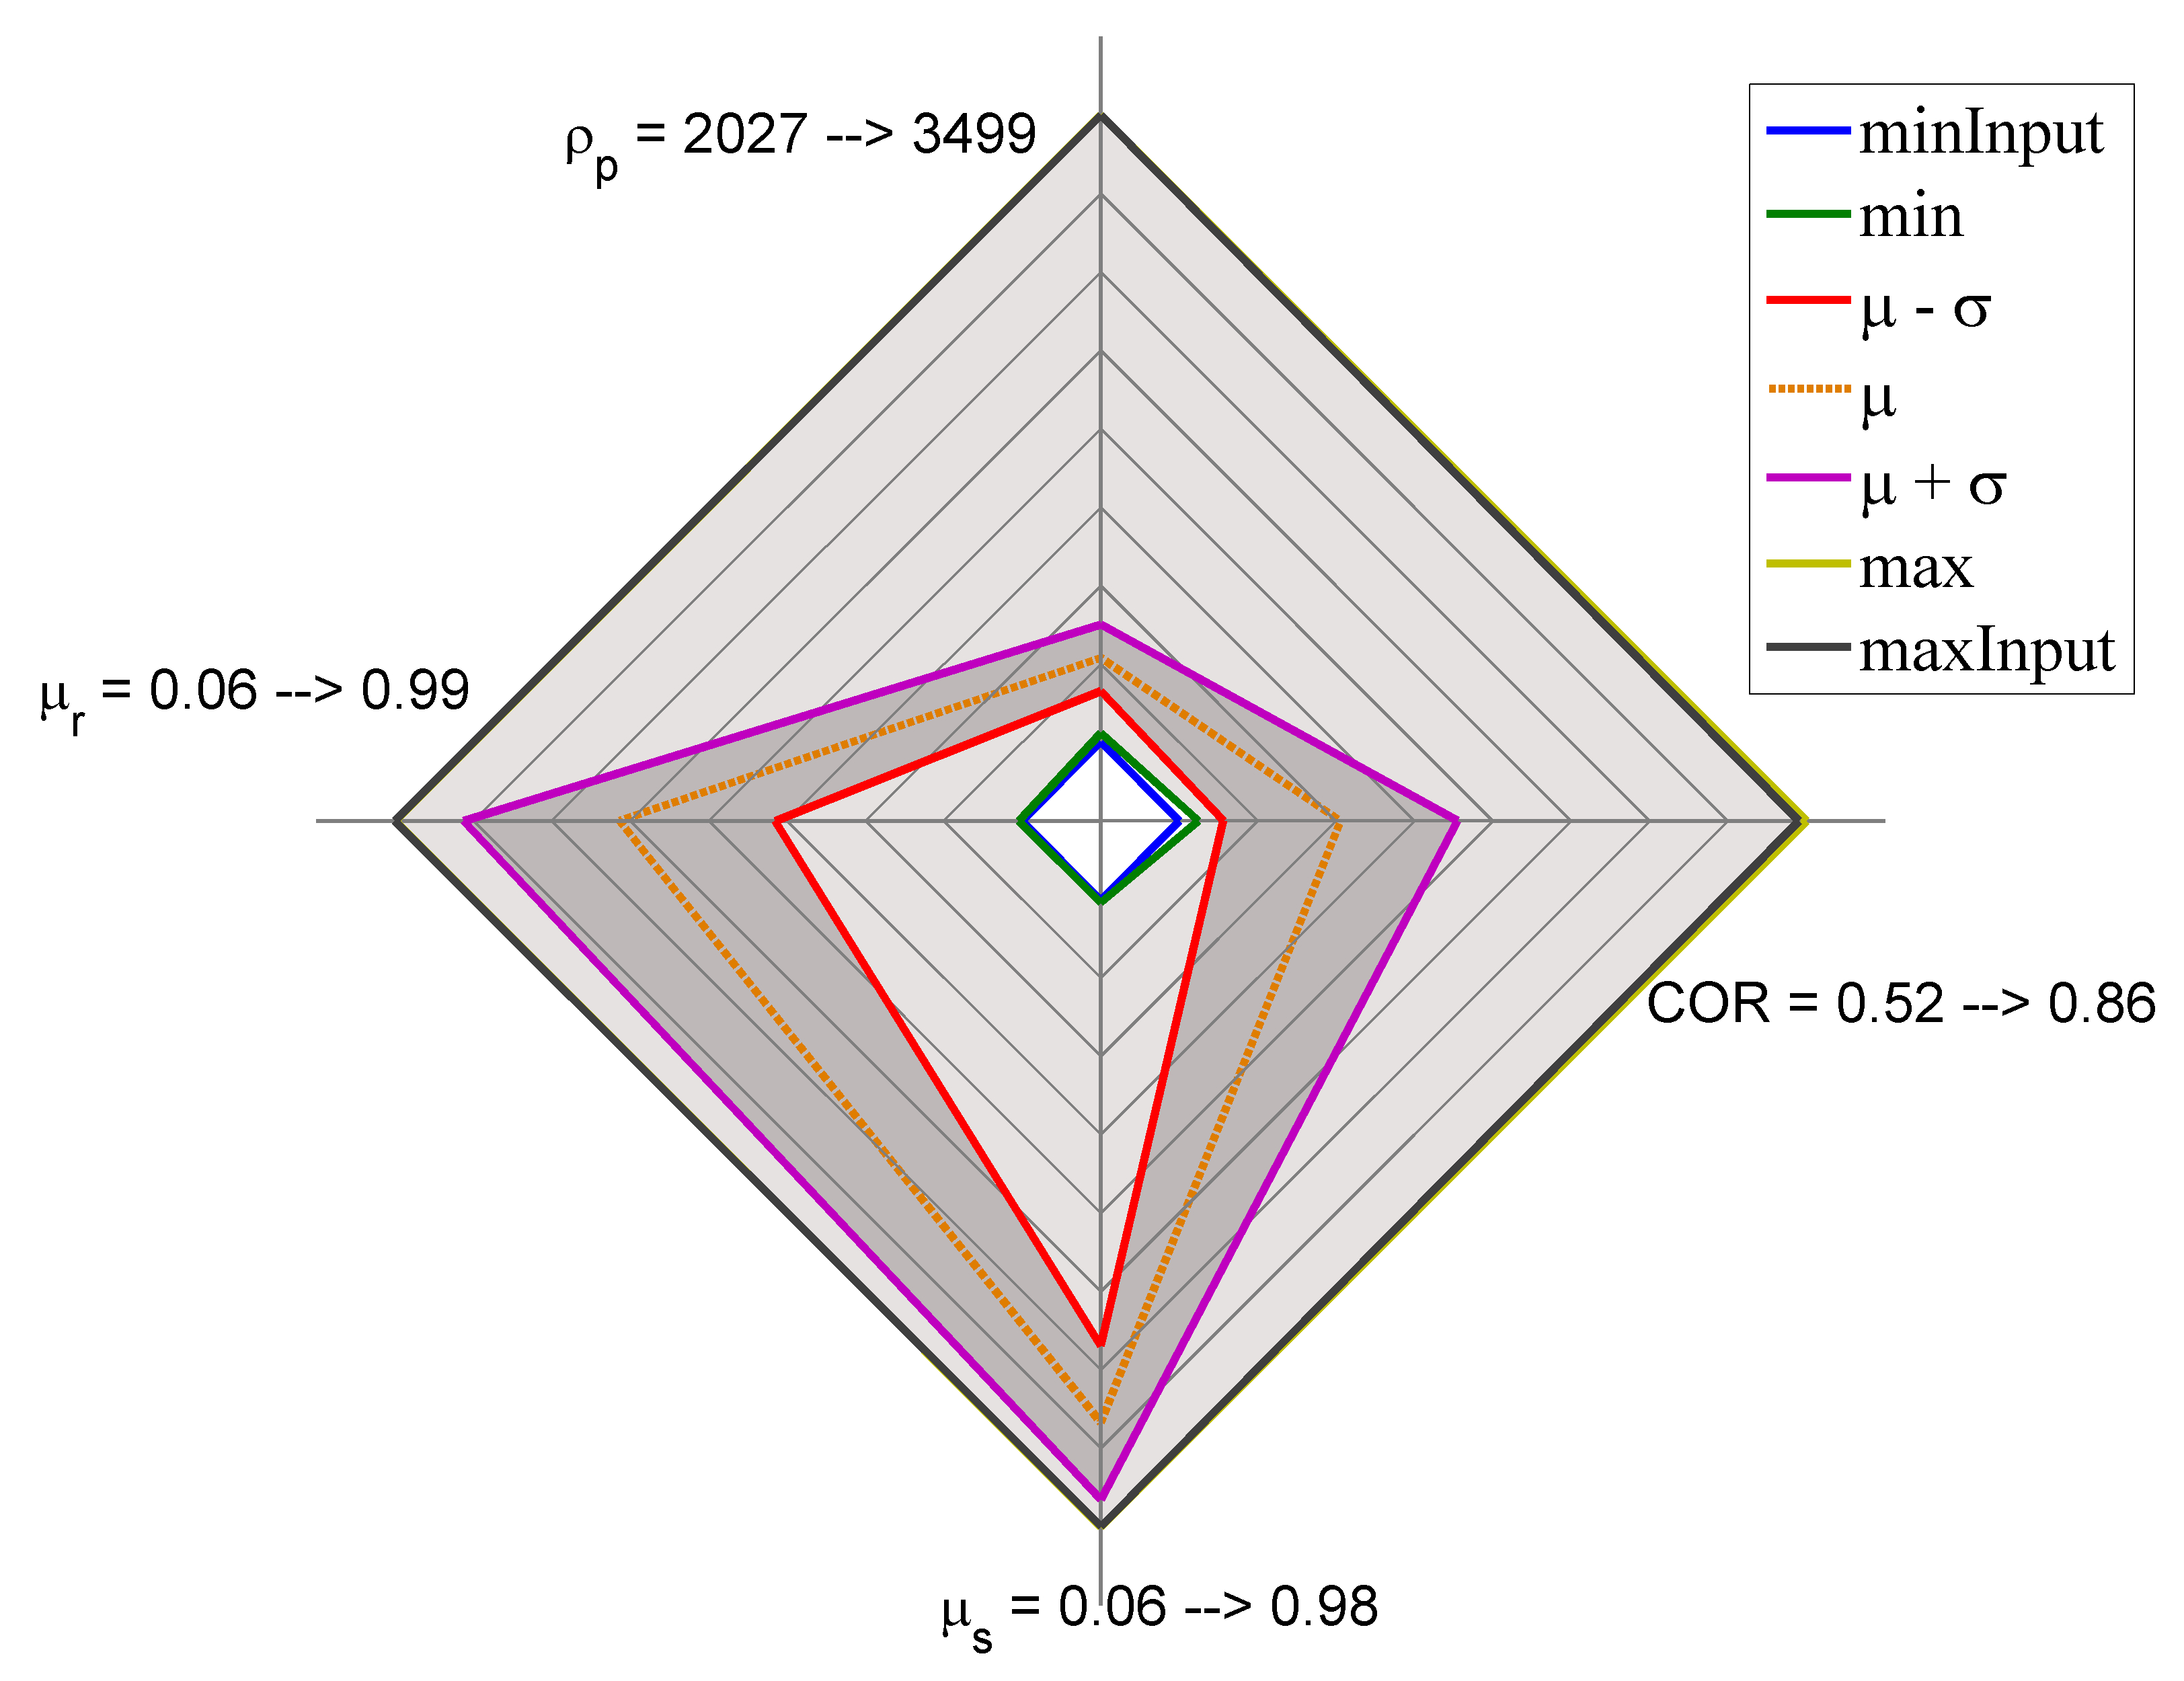
\includegraphics[width=0.5\columnwidth]{images/original/26radarpirker08schulze10070}
        \caption{Radar plot, $SCT$, $\sigma_n=10070 ~[Pa]$, $P=0.8$}
        \label{fig:26radarpirker08schulze10070} 
    \end{subfigure}\\
        \begin{subfigure}
        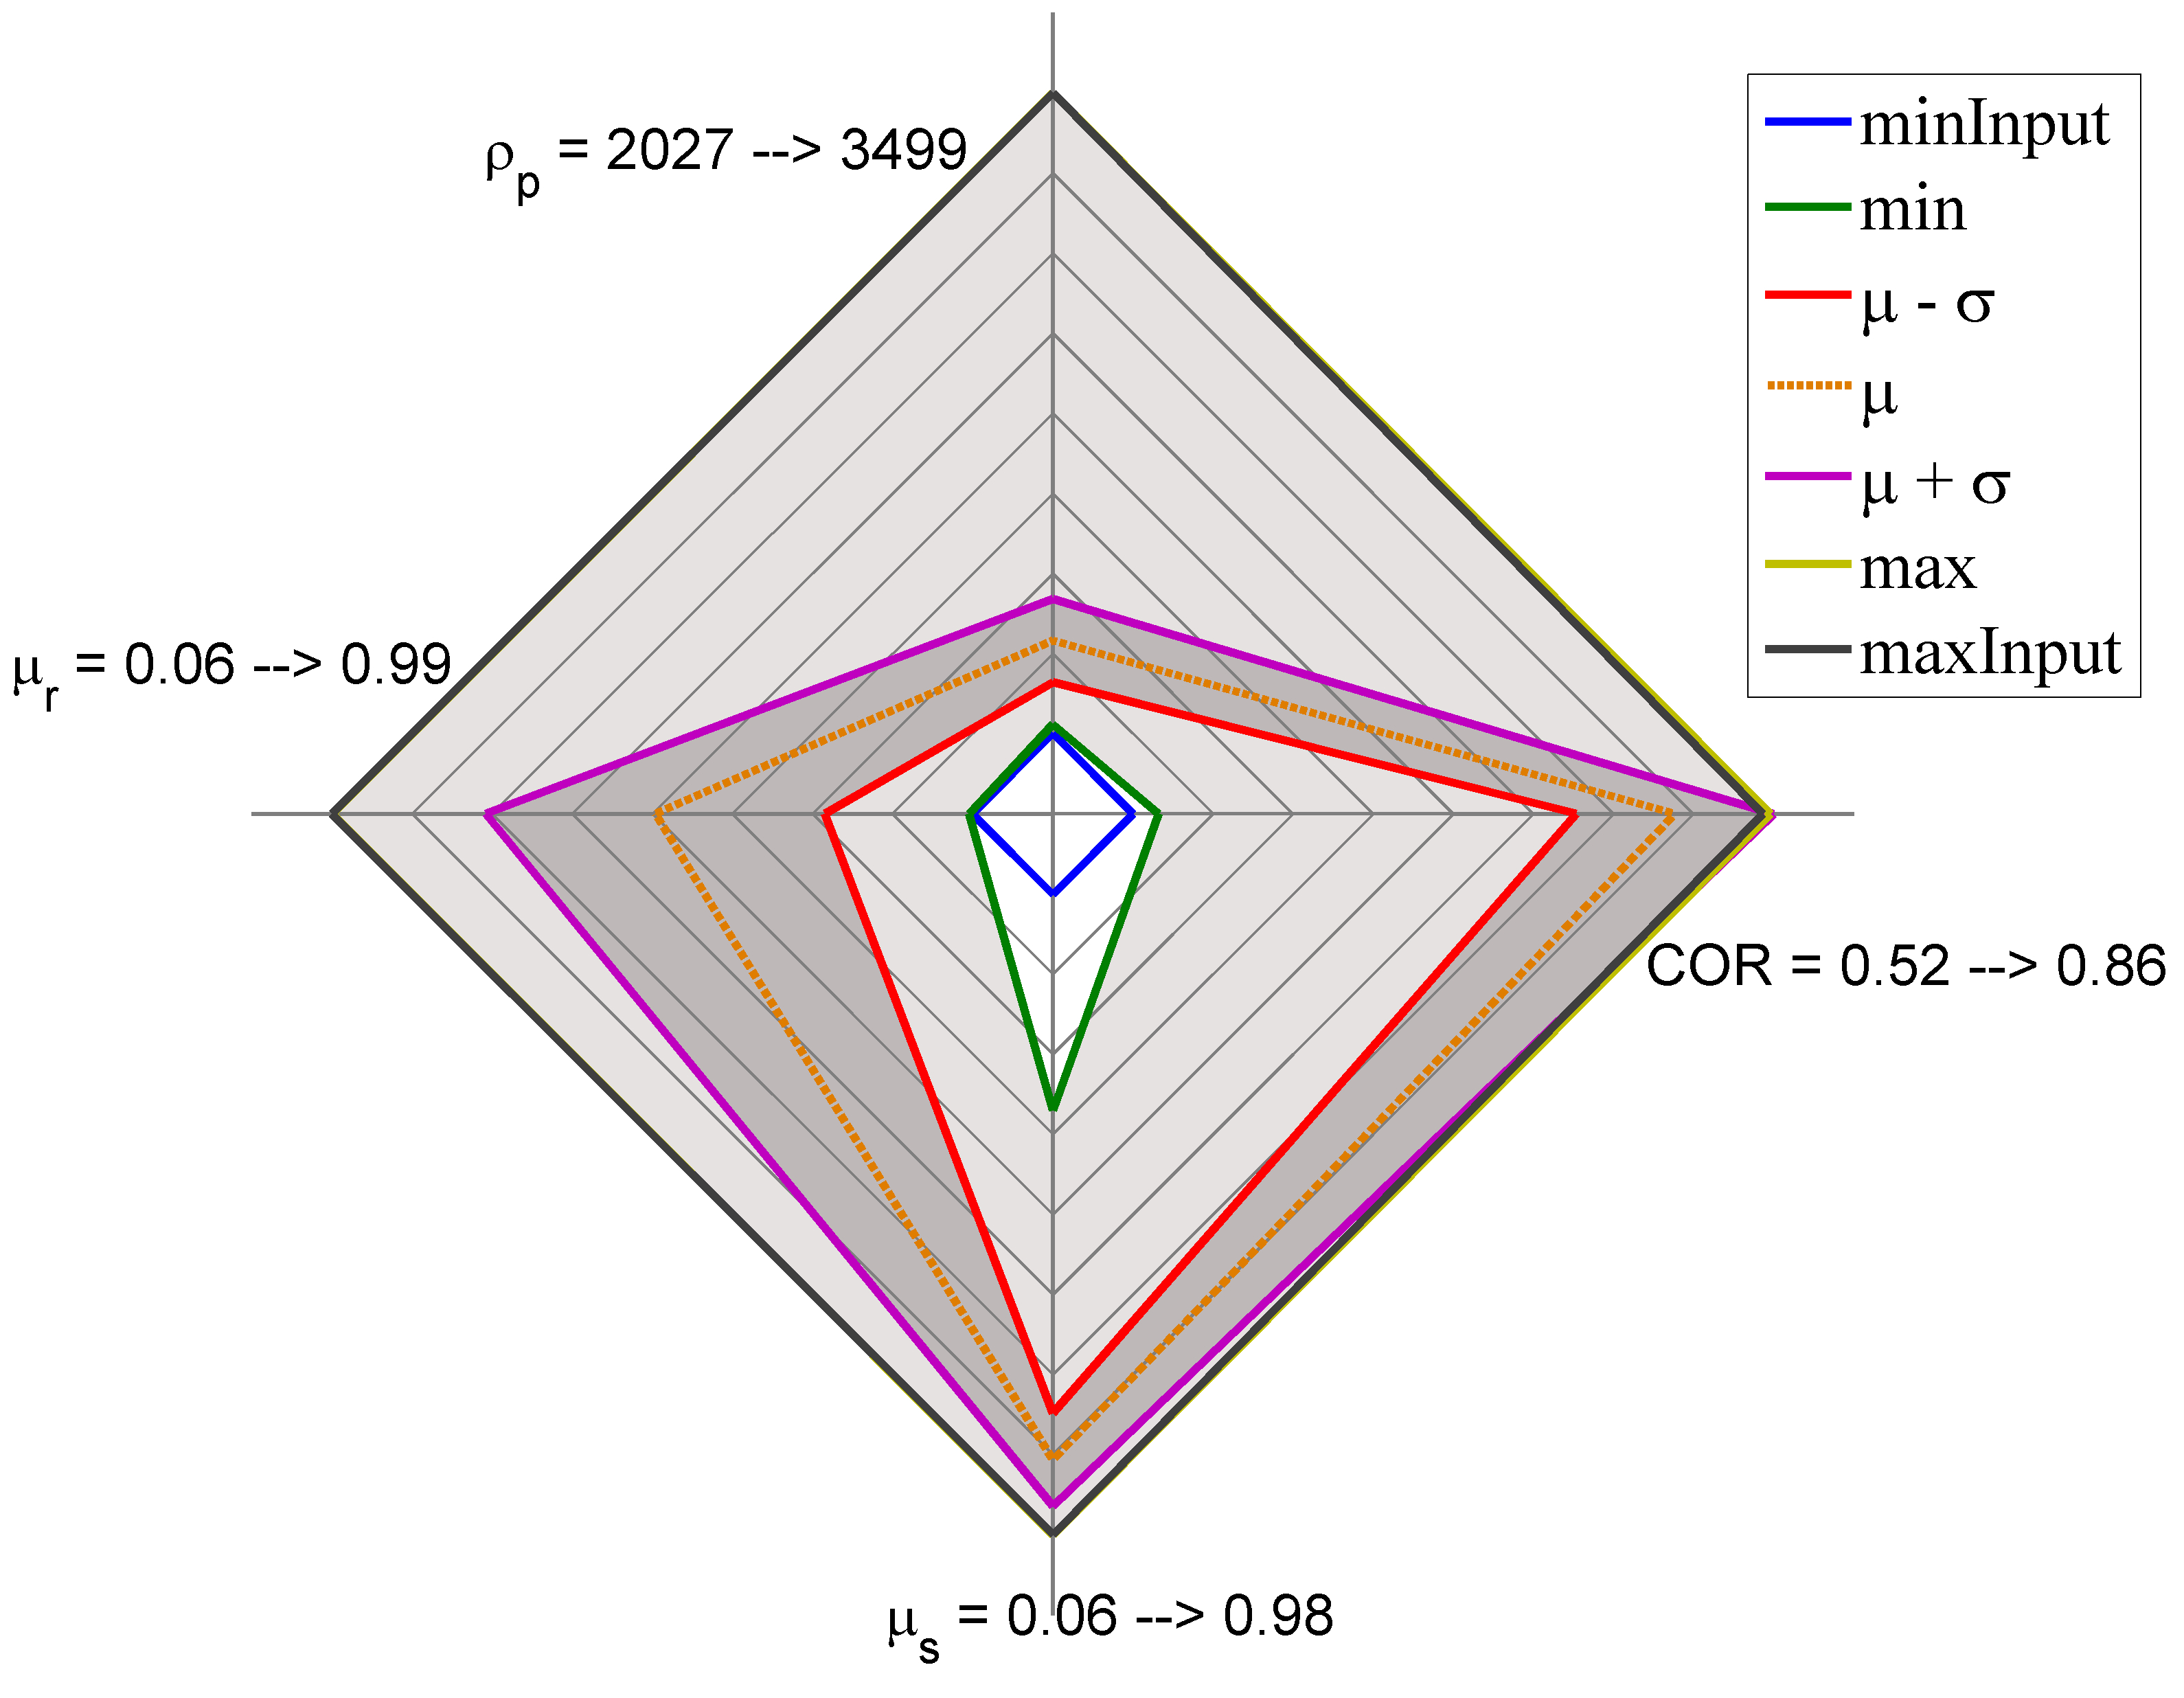
\includegraphics[width=0.5\columnwidth]{images/original/28radarpirker12schulze10070}
        \caption{Radar plot, $SCT$, $\sigma_n=10070 ~[Pa]$, $P=1.2$}
        \label{fig:28radarpirker12schulze10070} 
    \end{subfigure}
    \caption[Radar plot of valid simulations parameters for three different
    bulk behaviours measured by SCT]{Radar plot of valid simulations parameters for three different
    bulk behaviours measured by shear cell tester ($SCT$).
    Each axes of the radar plot represents one simulation parameters.
    Furthermore, the shaded area represents valid parameters combinations.
    Dark shaded values stand for the confidence range.
    We represent the tabbed combinations for one load condition of the shear cell. 
    Further explanation in the text.
   }
    \label{fig:29schulzeradarandcloud}
\end{figure}
% 
% The minimum and maximum values, together with the mean and the confidence range,
% provided by the square deviation, are shown.
%     Here, the values plotted are selected between the numerical
%     values from the $NN$ with initially the original experimental results for the shear cell tester $P=1.0$ (Fig.
%     \ref{fig:24radarpirker1schulze10070}). 
%     The confidence range is large, especially for the $COR$.
%     Instead, both the $\rho_p$  and the $\mu_s$ show a narrow confidence range. 
%     Later, they have been chosen with  
%     the virtual decreased results $P=0.8$
%     (\ref{fig:26radarpirker08schulze10070}).
%     The confidence range is narrower compared to $P=1.0$
%     The last image (Fig. \ref{fig:28radarpirker12schulze10070}) represents
%     instead the selection with the the virtual increased results $P=1.2$.
%     The plot shows a largely different confidence range. 
\begin{figure}[htp] \centering

    \begin{subfigure}[b]{0.96\columnwidth}
        \includegraphics[width=\textwidth]{27cloudpirker08schulze10070}
        \caption{Cloud plot, $SSC$, $\sigma_n=10070 ~[Pa]$, $P=0.8$}
        \label{fig:27cloudpirker08schulze10070} 
    \end{subfigure}\\
    \begin{subfigure}[b]{0.96\columnwidth}
        \includegraphics[width=\textwidth]{25cloudpirker1schulze10070}
        \caption{Cloud plot, $SSC$, $\sigma_n=10070 ~[Pa]$, $P=1.0$}
        \label{fig:25cloudpirker1schulze10070}
    \end{subfigure}\\

    \begin{subfigure}[b]{0.96\columnwidth}
        \includegraphics[width=\textwidth]{30cloudpirker12schulze10070}
        \caption{Cloud plot, $SSC$, $\sigma_n=10070 ~[Pa]$, $P=1.2$}
        \label{fig:30cloudpirker12schulze10070} 
    \end{subfigure}
    \caption[Density plot comparison of SCT results]{Density plot comparison of
    shear cell tester ($SSC$) results. We represent the marked combinations for
    one load condition of the shear cell. 
    Density plot of the particles' coefficient of restitution (COR) in dependence
	of coefficient of sliding friction and coefficient of rolling friction; in the
	white area no valid sets of simulation parameter can be found.
	In each cell the valid sets are grouped accordingly to the 4 different COR
	ranges.
	Each cell is colored accordingly to the group with the most members. 
    Here, the values plotted are selected between the numerical
    values from the Neural Network with initially the original experimental
    results for the $SSC$, with a product coefficient $P=1.0$ (Fig.
    \ref{fig:25cloudpirker1schulze10070}). 
        Later, they have been chosen with  
    the virtual decreased results $P=0.8$
    (\ref{fig:27cloudpirker08schulze10070}).
    The last image (Fig. \ref{fig:30cloudpirker12schulze10070}) represents
    instead the selection with the the virtual increased results $P=1.2$.    }
    \label{fig:29schulzeradarandcloud}
\end{figure}
\begin{figure}[htp] \centering
    \begin{subfigure}[b]{0.96\columnwidth}
        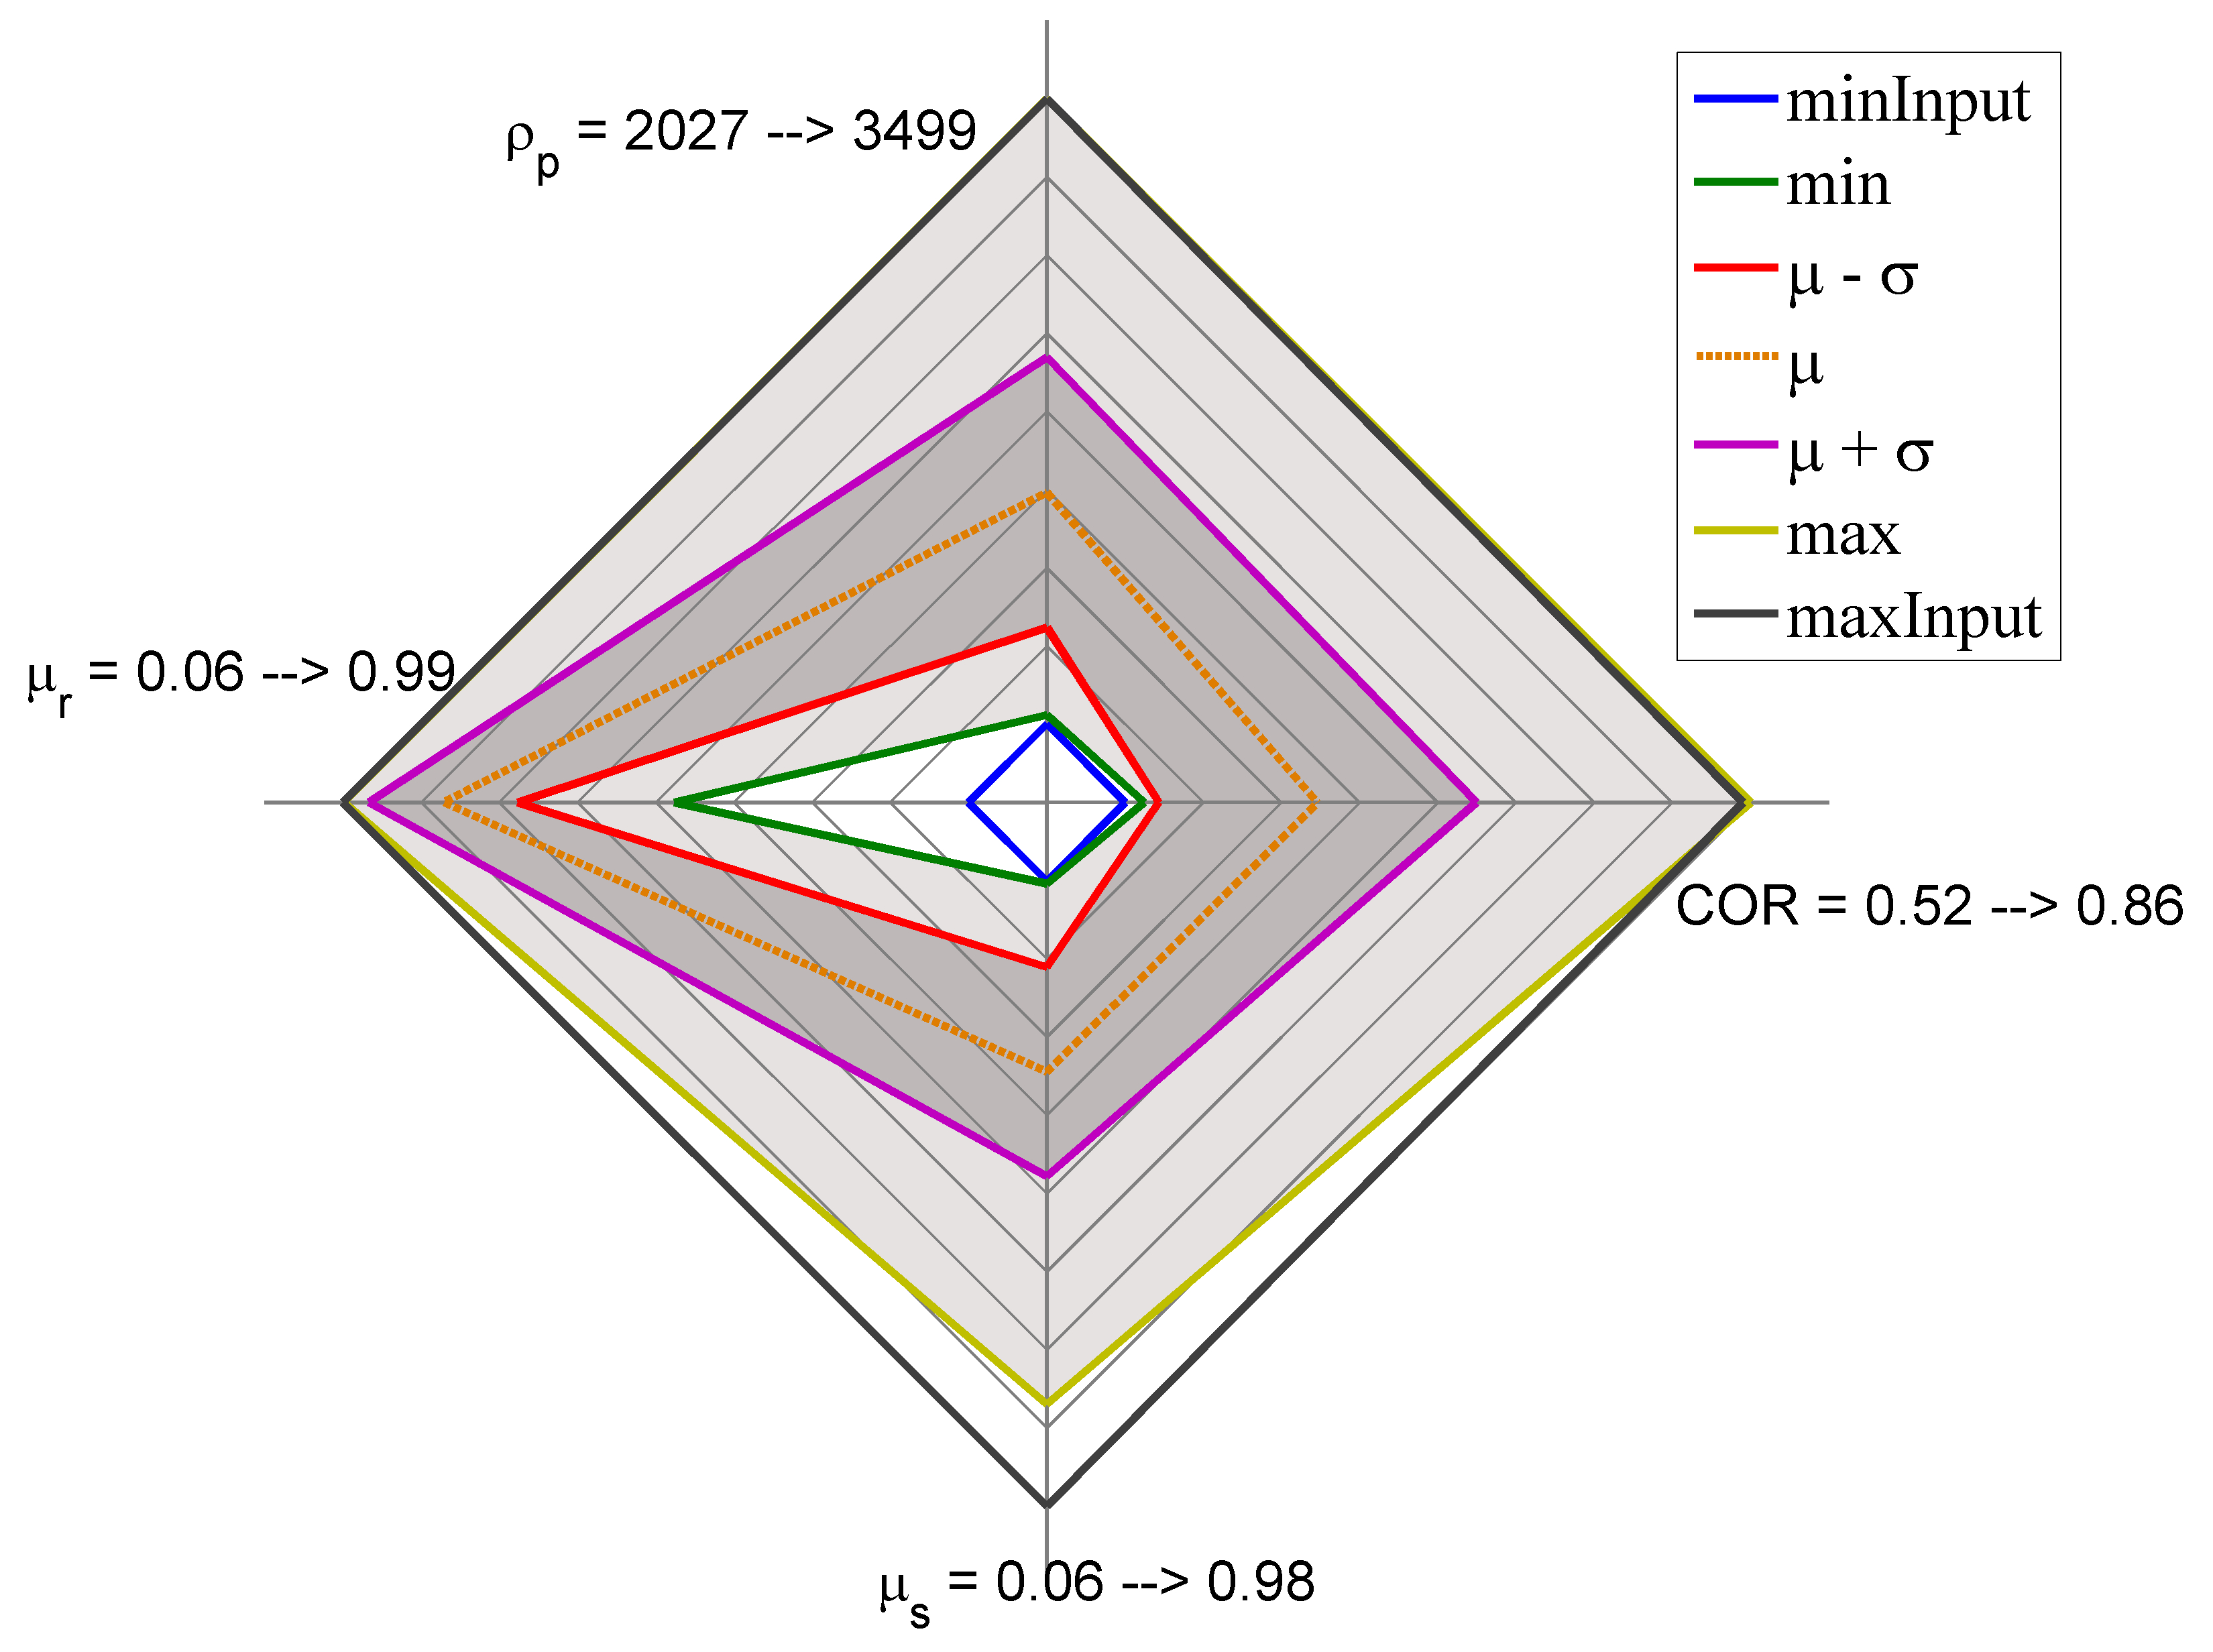
\includegraphics[width=\textwidth]{images/original/31radarpirker1aor}
        \caption{Radar plot, $AOR_{exp} = 38.85 ^\circ$}
        \label{fig:31radarpirker1aor} 
    \end{subfigure}\\
        \begin{subfigure}[b]{0.96\columnwidth}
        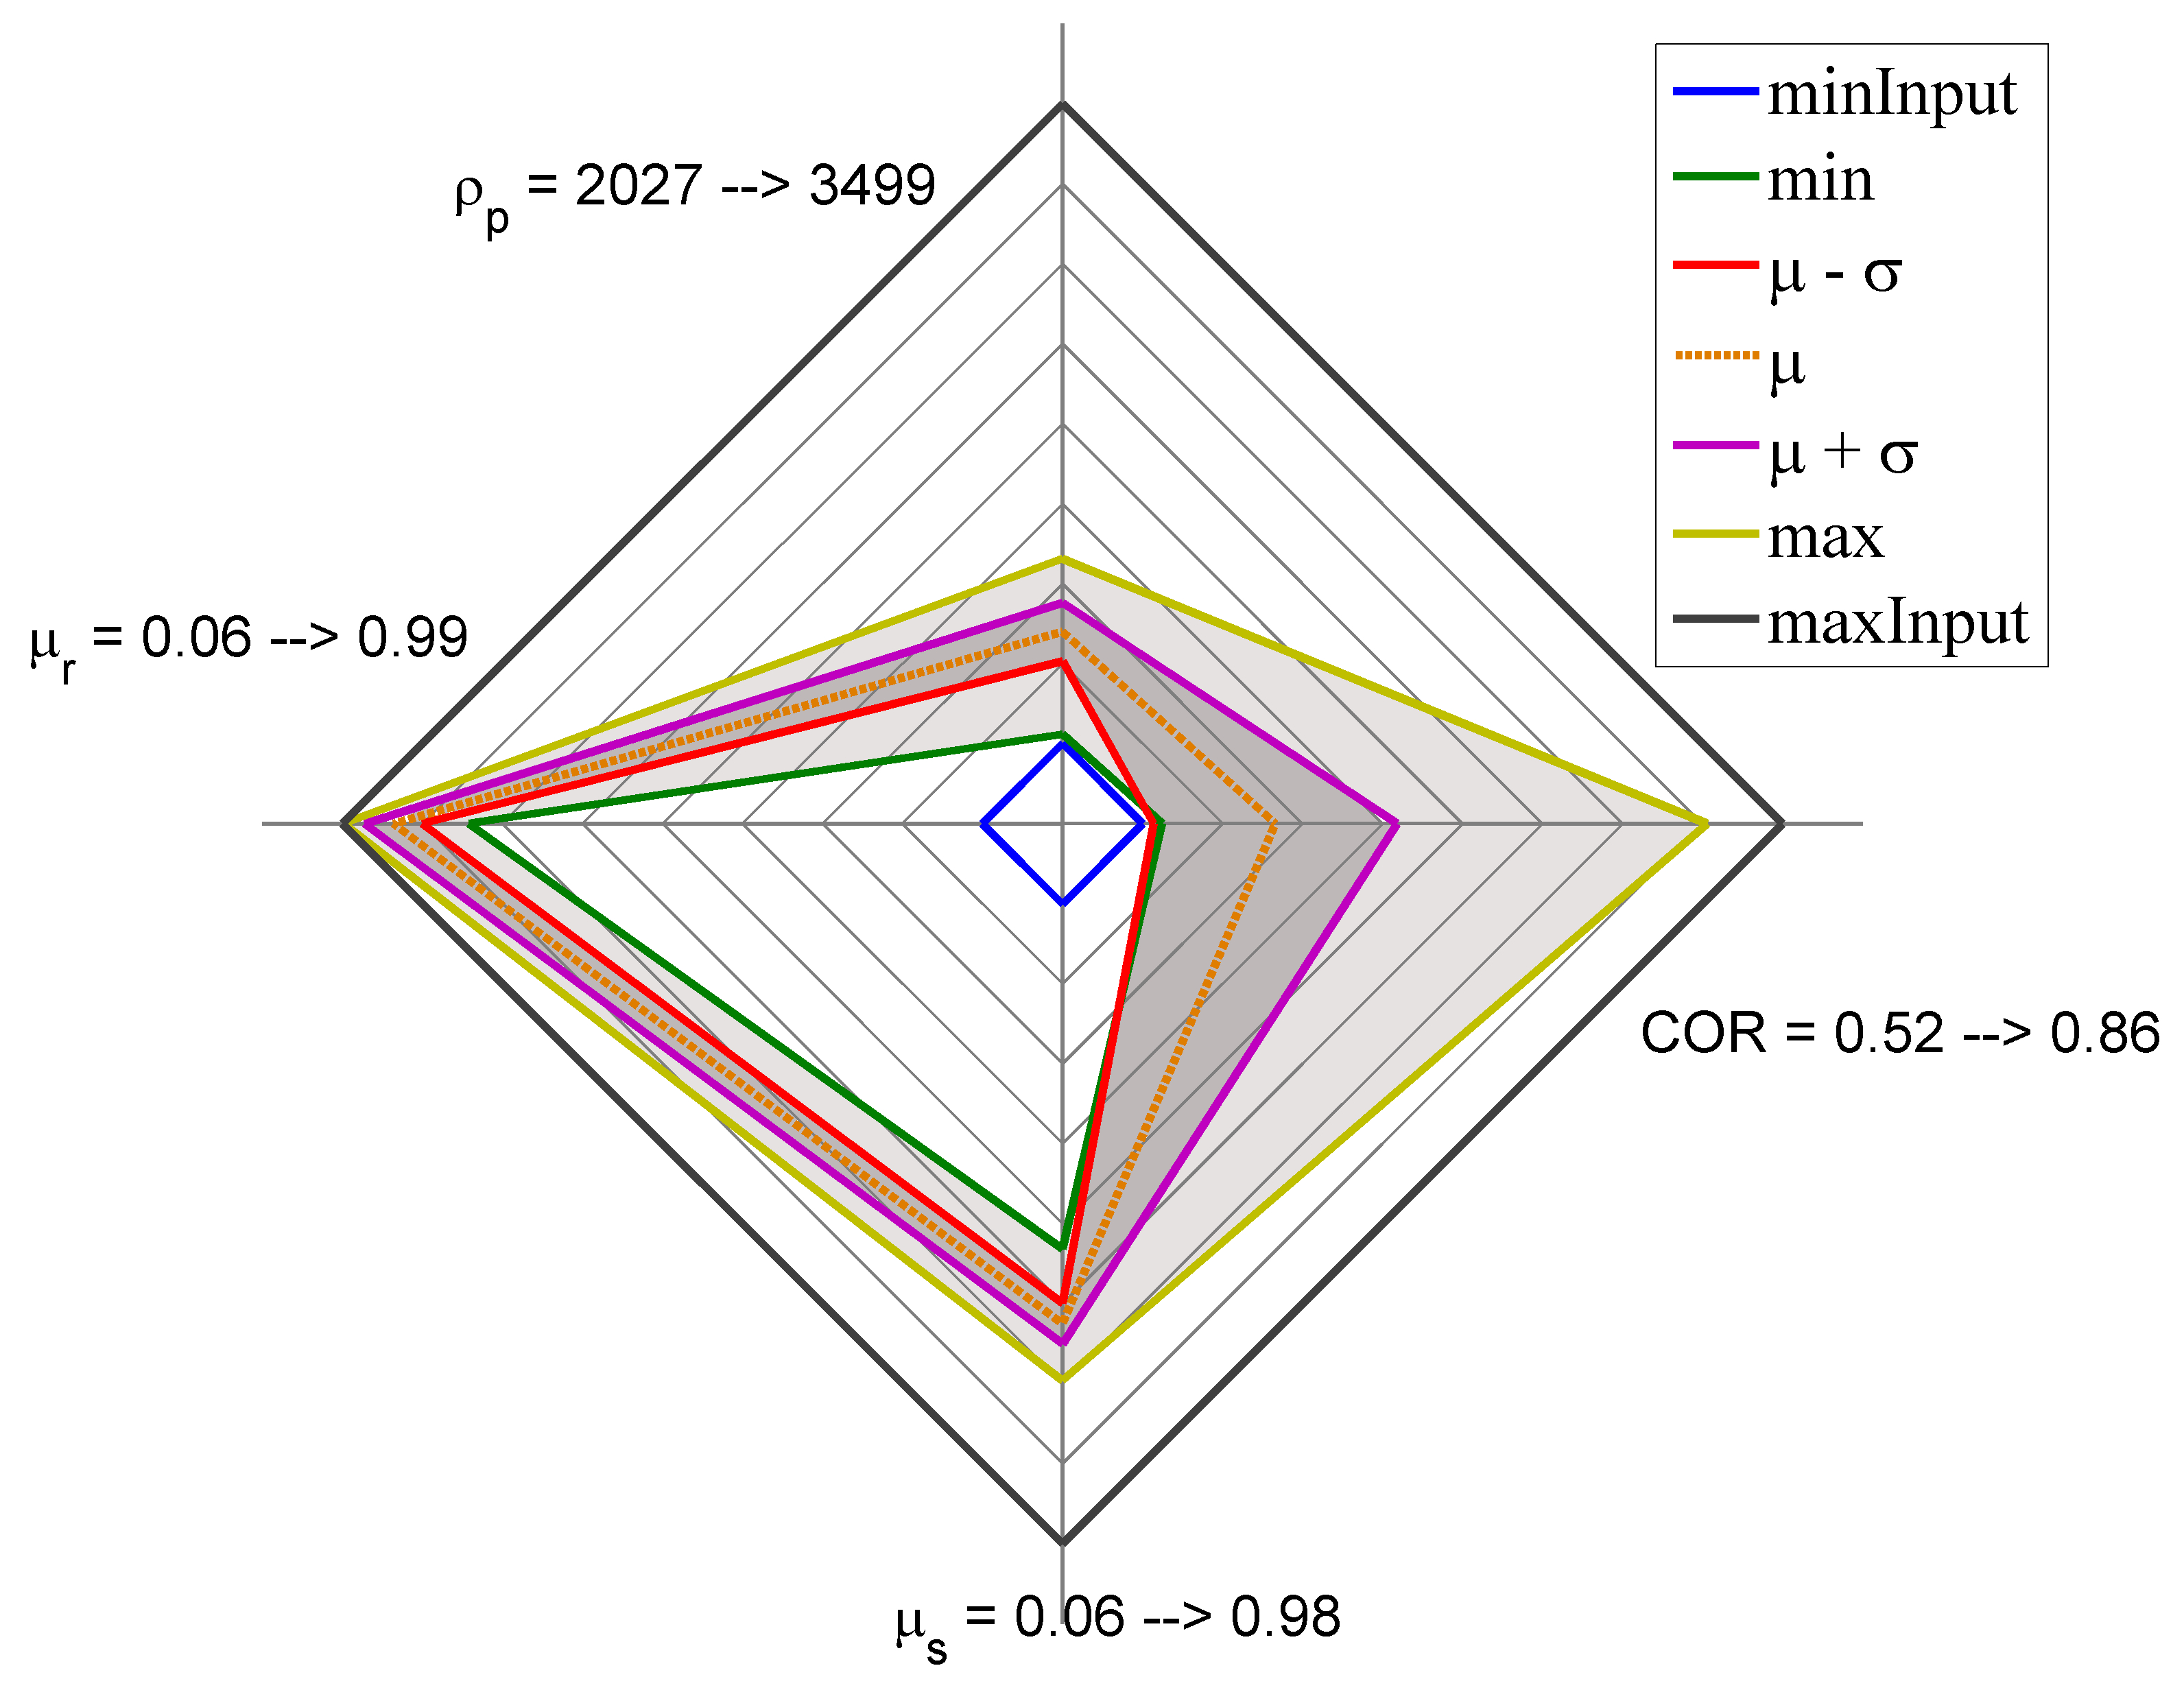
\includegraphics[width=\textwidth]{images/original/33radarpirker1schulze10070aor}
        \caption{Radar plot, $AOR_{exp} = 38.85
        ^\circ$, $SCT$, $\sigma_n=10070 ~[Pa]$}
        \label{fig:33radarpirker1schulze10070aor} 
    \end{subfigure}
    \caption[Radar plot comparison of AOR and SCT results]{Radar plot comparison
    of $AOR$ and $SCT$ results. We represent the tabbed combinations for the
    $AOR$ test.
    The minimum and maximum values, together with the mean and the confidence
	range, provided by the square deviation, are shown.
    Here, the values plotted are selected between the numerical
    values from the $NN$ with initially the original experimental results for
    the $AOR$, $P=1.0$ (Fig.
    \ref{fig:31radarpirker1aor}). 
    The confidence range is large, except for the $\mu_r$.
    The last image (Fig. \ref{fig:33radarpirker1schulze10070aor}) represents
    instead the values valid for both the $AOR$ test and the $SCT$, with a
    $\sigma_n=10070 ~[Pa]$, both for $P=1.0$.
    The range is meager, except for the $COR$.    }
    \label{fig:35schulze10070aorradarandcloud}
\end{figure}
\begin{figure}[htp] \centering
    \begin{subfigure}[b]{0.96\columnwidth}
        \includegraphics[width=\textwidth]{images/original/32cloudpirker1aor}
        \caption{Cloud plot, $AOR_{exp} = 38.85 ^\circ$}
        \label{fig:32cloudpirker1aor} 
    \end{subfigure}\\
    \begin{subfigure}[b]{0.96\columnwidth}
        \includegraphics[width=\textwidth]{images/original/34cloudpirker1schulze10070aor}
        \caption{Cloud plot, $AOR_{exp} = 38.85
        ^\circ$ \& $SCT$: $\sigma_n=10070 ~[Pa]$}
        \label{fig:34cloudpirker1schulze10070aor} 
    \end{subfigure}
    \caption[Density plot comparison of AOR and SCT results]{Density plot
    comparison of $AOR$ and $SCT$ results. We represent the tabbed combinations for the
    $AOR$ test.
    Density plot of the particles' coefficient of restitution (COR) in dependence
	of coefficient of sliding friction and coefficient of rolling friction; in the
	white area no valid sets of simulation parameter can be found.
	In each cell the valid sets are grouped accordingly to the 4 different COR
	ranges.
	Each cell is colored accordingly to the group with the most members. 
    Here, the values plotted are selected between the numerical
    values from the $NN$ with initially the original experimental results for
    the $AOR$, $P=1.0$ (Fig.
    \ref{fig:32cloudpirker1aor}). 
    The last image (Fig. \ref{fig:34cloudpirker1schulze10070aor}) represents
    instead the values valid for both the $AOR$ test and the $SCT$, with a
    $\sigma_n=10070 ~[Pa]$, both for $P=1.0$. }
    \label{fig:35schulze10070aorradarandcloud}
\end{figure}


%\begin{figure}[!h] 
\centering 
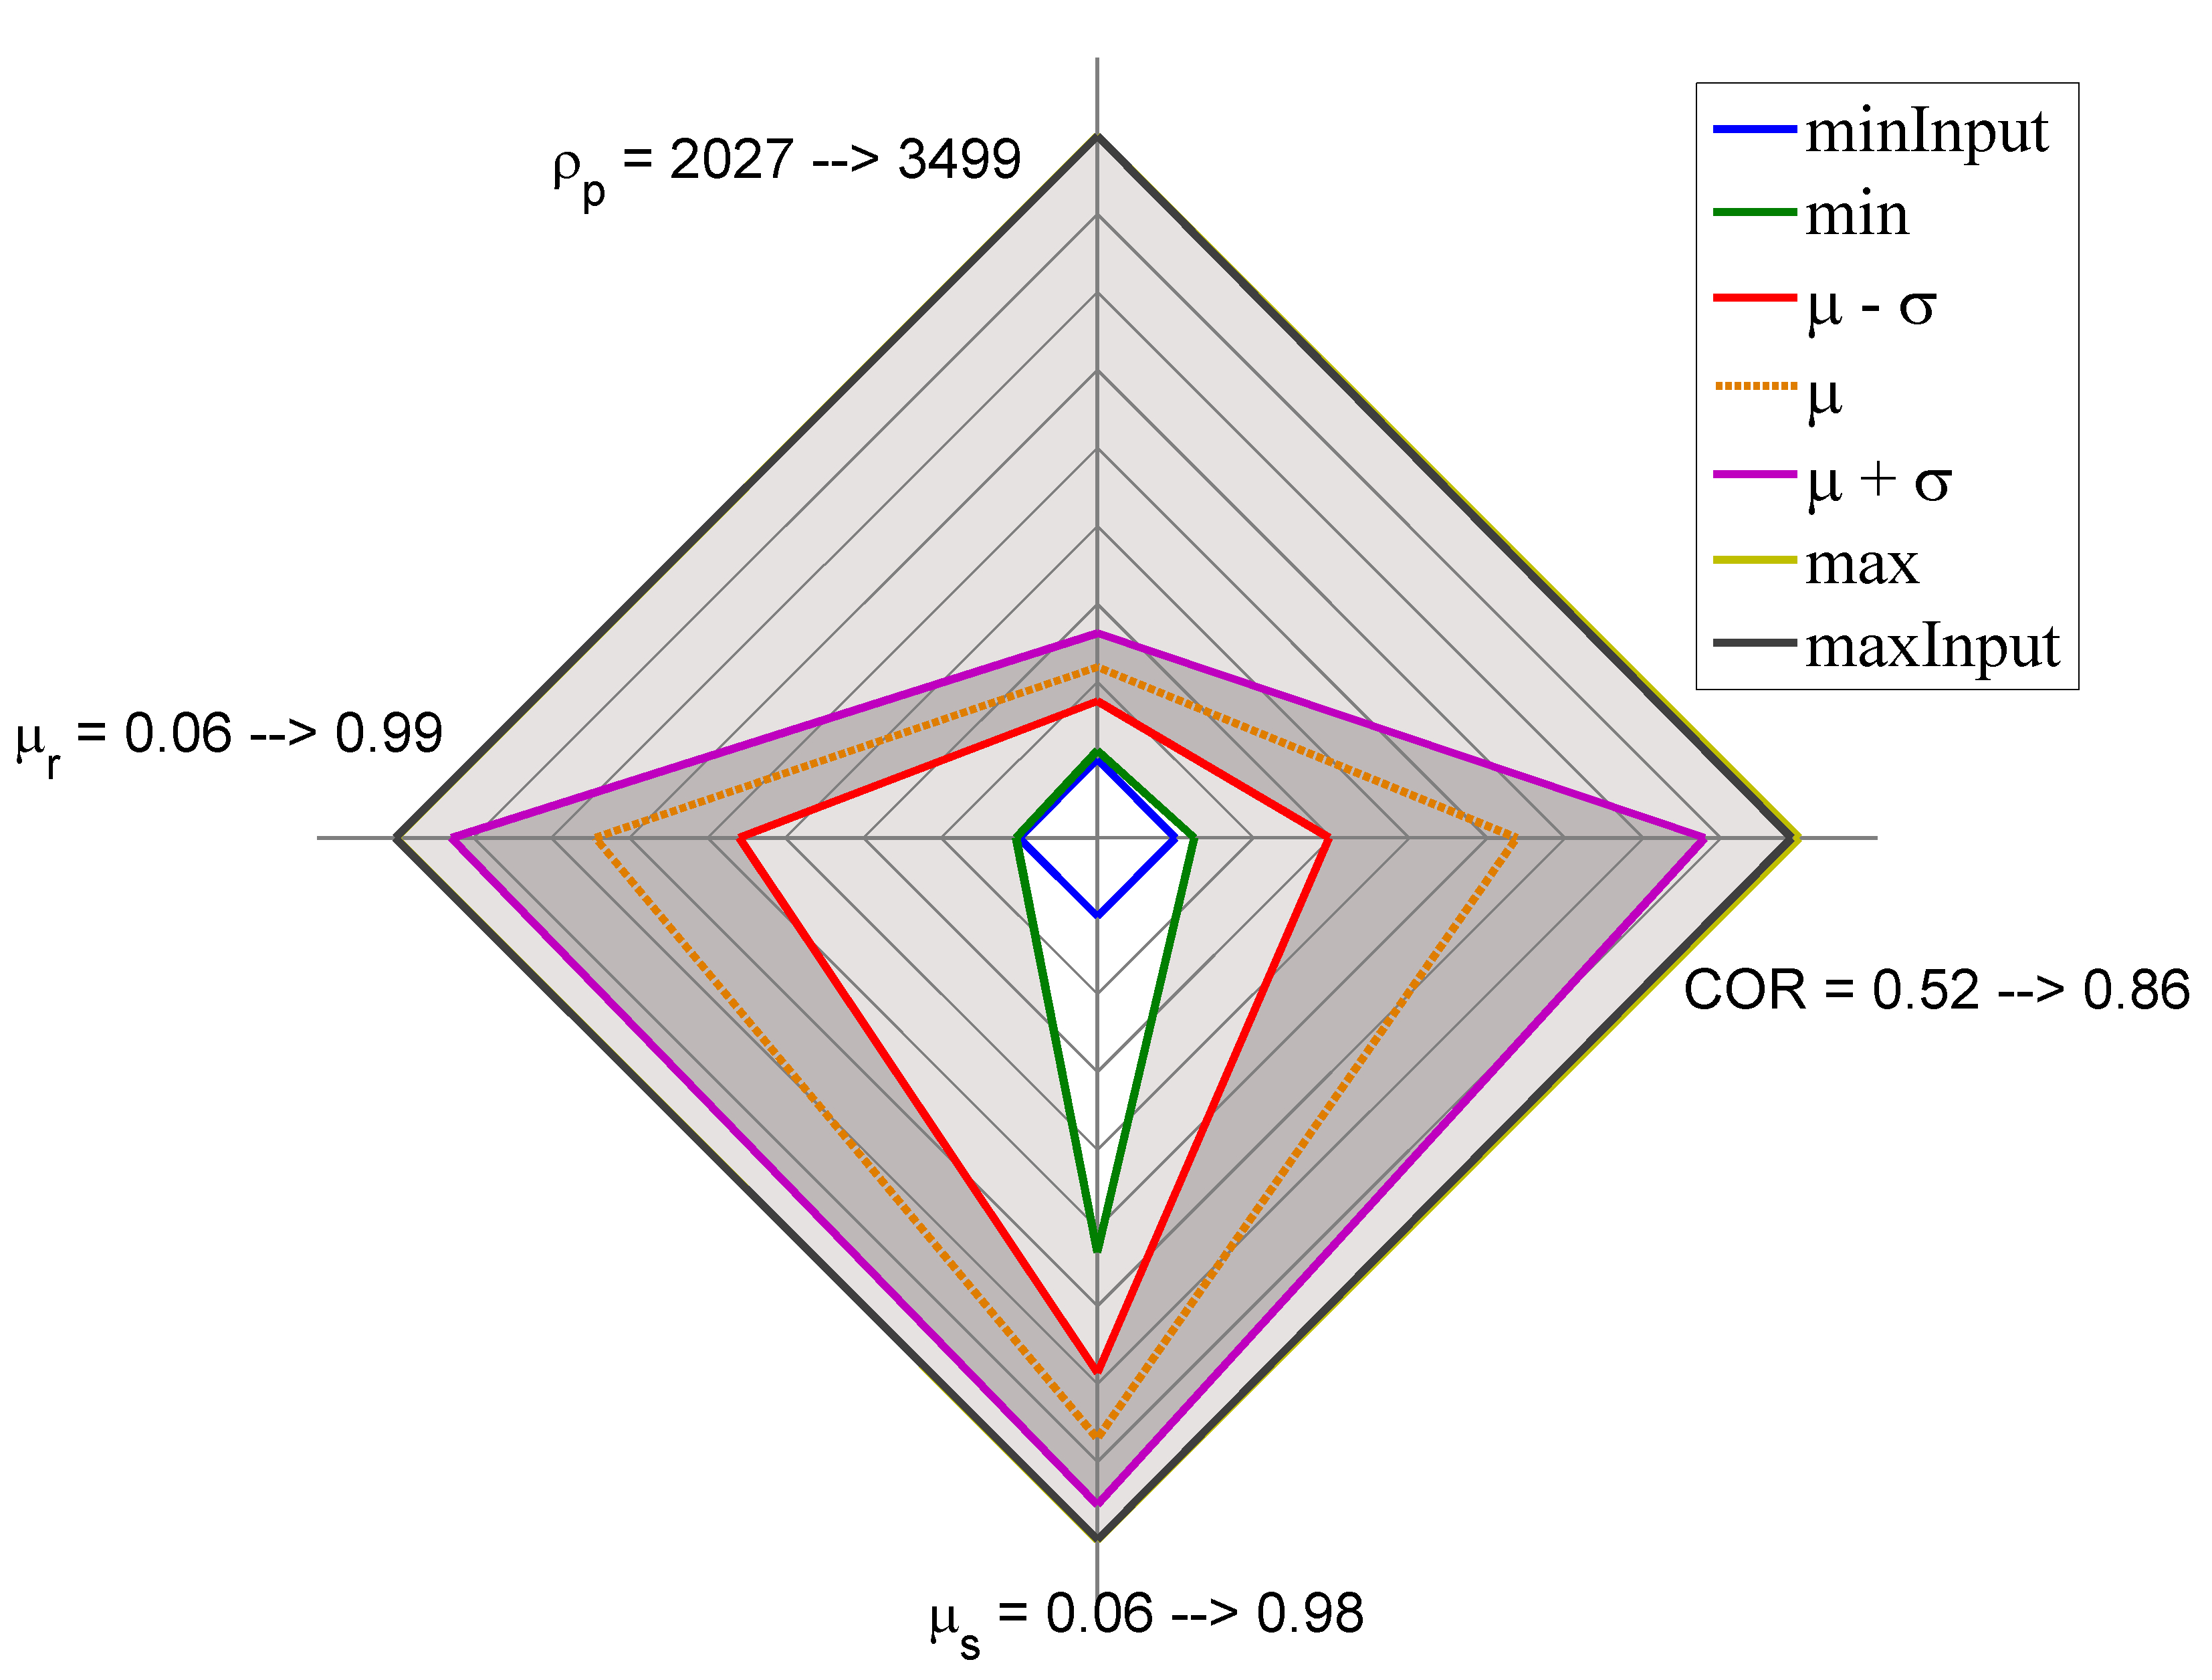
\includegraphics[height=0.40\columnwidth]{images/original/24radarpirker1schulze10070}
%[width=.96\textwidth]
\caption{Radar P1 Schulze10070}
\label{fig:24radarpirker1schulze10070} 
\end{figure}

%SCT: sn = 10070 [Pa], coeff. P. = 1
% \begin{figure}[htp]
%     \centering
%     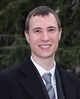
\includegraphics[width=.2\textwidth]{images/vitae/lbenvenuti}
%     \caption{OpenMP, MPI, MPI/OpenMP Hybrid runs of Box in a box testcase on 32
%     cores. The OpenMP-only run suffers from limited memory bandwidth in
%     memory-bound algorithms inside of the Modify section of the code. MPI-only has
%     low averaged runtimes for each section, but a very large Other timing, which
%     hints for a large amount of load-imbalance. Hybrid timings are a bit worse
%     on average, but because of better balancing, processes have lower wait times
%     inside of Other timing.}
% 	\label{fig:boxInBoxComparison}

%\begin{figure}[!h] 
\centering 
\includegraphics[height=0.33\columnwidth]{images/original/25cloudpirker1schulze10070}
%[width=.96\textwidth]
\caption{Cloud P1 Schulze10070}
\label{fig:25cloudpirker1schulze10070} 
\end{figure}

%SCT: sn = 10070 [Pa], coeff. P. = 1
% \begin{figure}[htp]
%     \centering
%     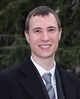
\includegraphics[width=.2\textwidth]{images/vitae/lbenvenuti}
%     \caption{OpenMP, MPI, MPI/OpenMP Hybrid runs of Box in a box testcase on 32
%     cores. The OpenMP-only run suffers from limited memory bandwidth in
%     memory-bound algorithms inside of the Modify section of the code. MPI-only has
%     low averaged runtimes for each section, but a very large Other timing, which
%     hints for a large amount of load-imbalance. Hybrid timings are a bit worse
%     on average, but because of better balancing, processes have lower wait times
%     inside of Other timing.}
% 	\label{fig:boxInBoxComparison}

%\begin{figure}[!h] 
\centering 
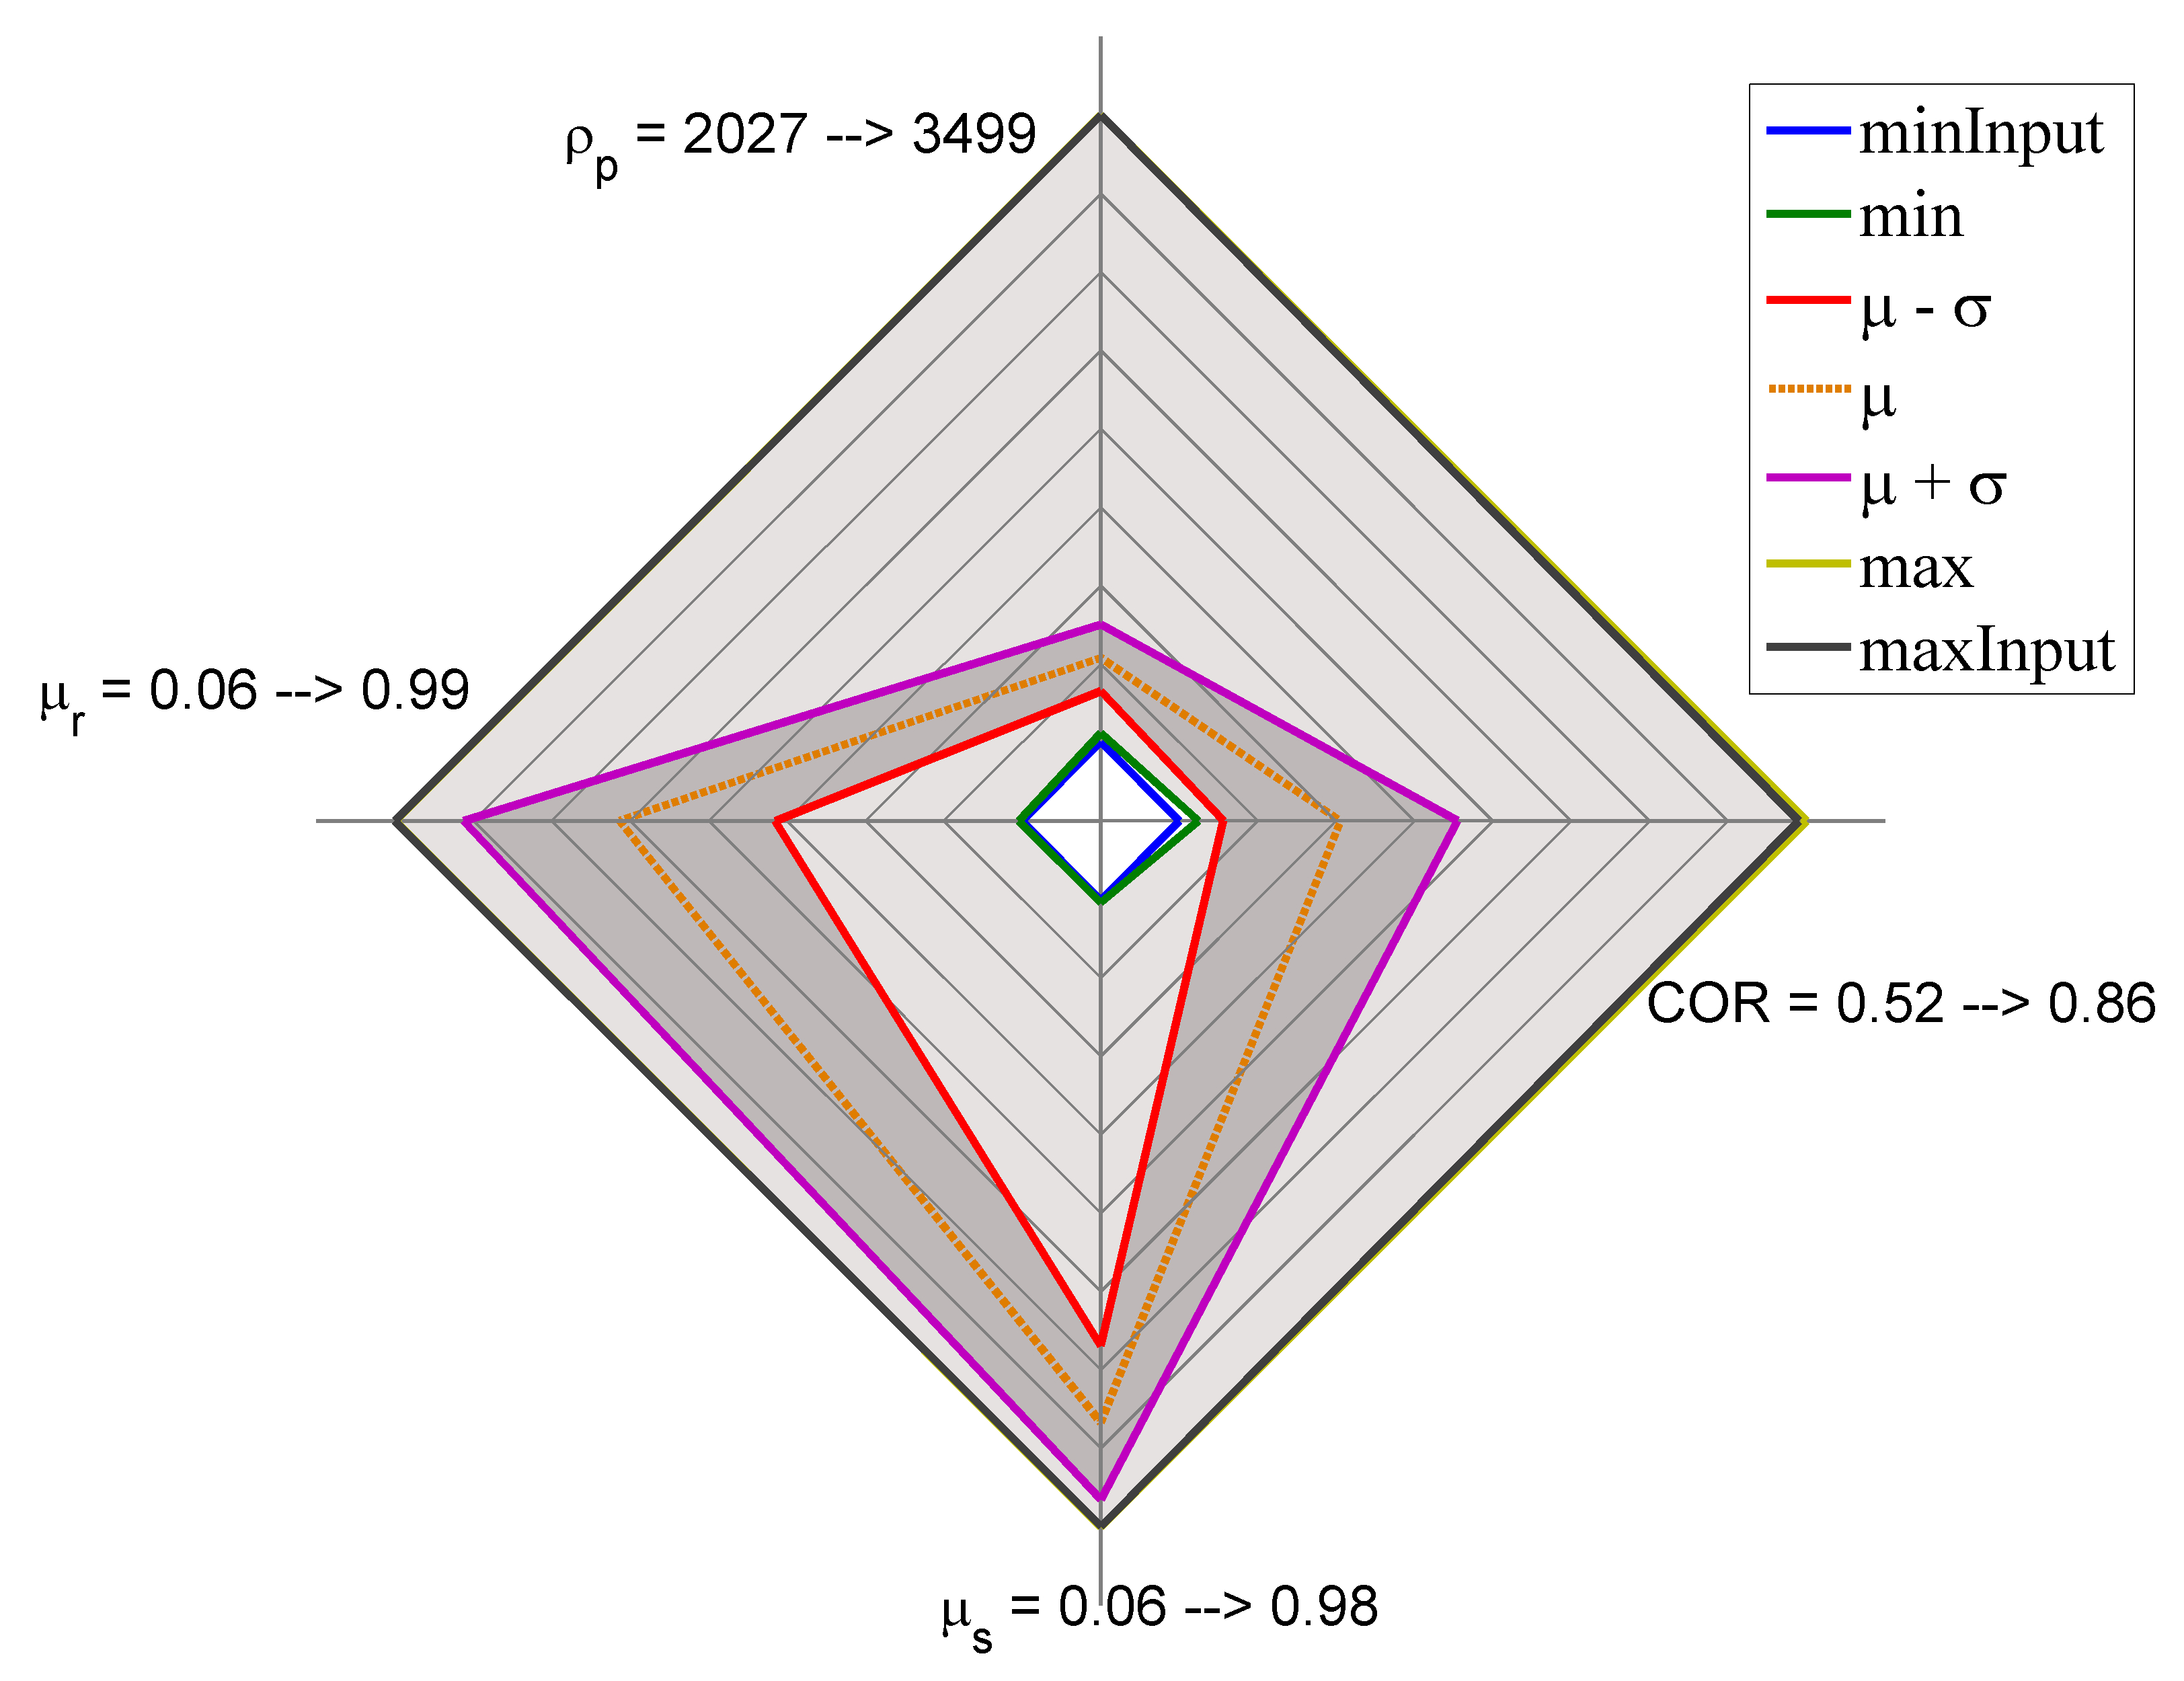
\includegraphics[height=3in]{images/original/26radarpirker08schulze10070}
%[width=.96\textwidth]
\caption{Radar P08 Schulze10070}
\label{fig:26radarpirker08schulze10070} 
\end{figure}

%SCT: sn = 10070 [Pa], coeff. P. = 0.8
% \begin{figure}[htp]
%     \centering
%     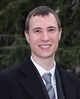
\includegraphics[width=.2\textwidth]{images/vitae/lbenvenuti}
%     \caption{OpenMP, MPI, MPI/OpenMP Hybrid runs of Box in a box testcase on 32
%     cores. The OpenMP-only run suffers from limited memory bandwidth in
%     memory-bound algorithms inside of the Modify section of the code. MPI-only has
%     low averaged runtimes for each section, but a very large Other timing, which
%     hints for a large amount of load-imbalance. Hybrid timings are a bit worse
%     on average, but because of better balancing, processes have lower wait times
%     inside of Other timing.}
% 	\label{fig:boxInBoxComparison}

%\begin{figure}[!h] 
\centering 
\includegraphics[height=3in]{images/original/27cloudpirker08schulze10070}
%[width=.96\textwidth]
\caption{Cloud P08 Schulze10070}
\label{fig:27cloudpirker08schulze10070} 
\end{figure}

%SCT: sn = 10070 [Pa], coeff. P. = 0.8
% \begin{figure}[htp]
%     \centering
%     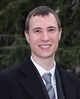
\includegraphics[width=.2\textwidth]{images/vitae/lbenvenuti}
%     \caption{OpenMP, MPI, MPI/OpenMP Hybrid runs of Box in a box testcase on 32
%     cores. The OpenMP-only run suffers from limited memory bandwidth in
%     memory-bound algorithms inside of the Modify section of the code. MPI-only has
%     low averaged runtimes for each section, but a very large Other timing, which
%     hints for a large amount of load-imbalance. Hybrid timings are a bit worse
%     on average, but because of better balancing, processes have lower wait times
%     inside of Other timing.}
% 	\label{fig:boxInBoxComparison}

%\begin{figure}[!h] 
\centering 
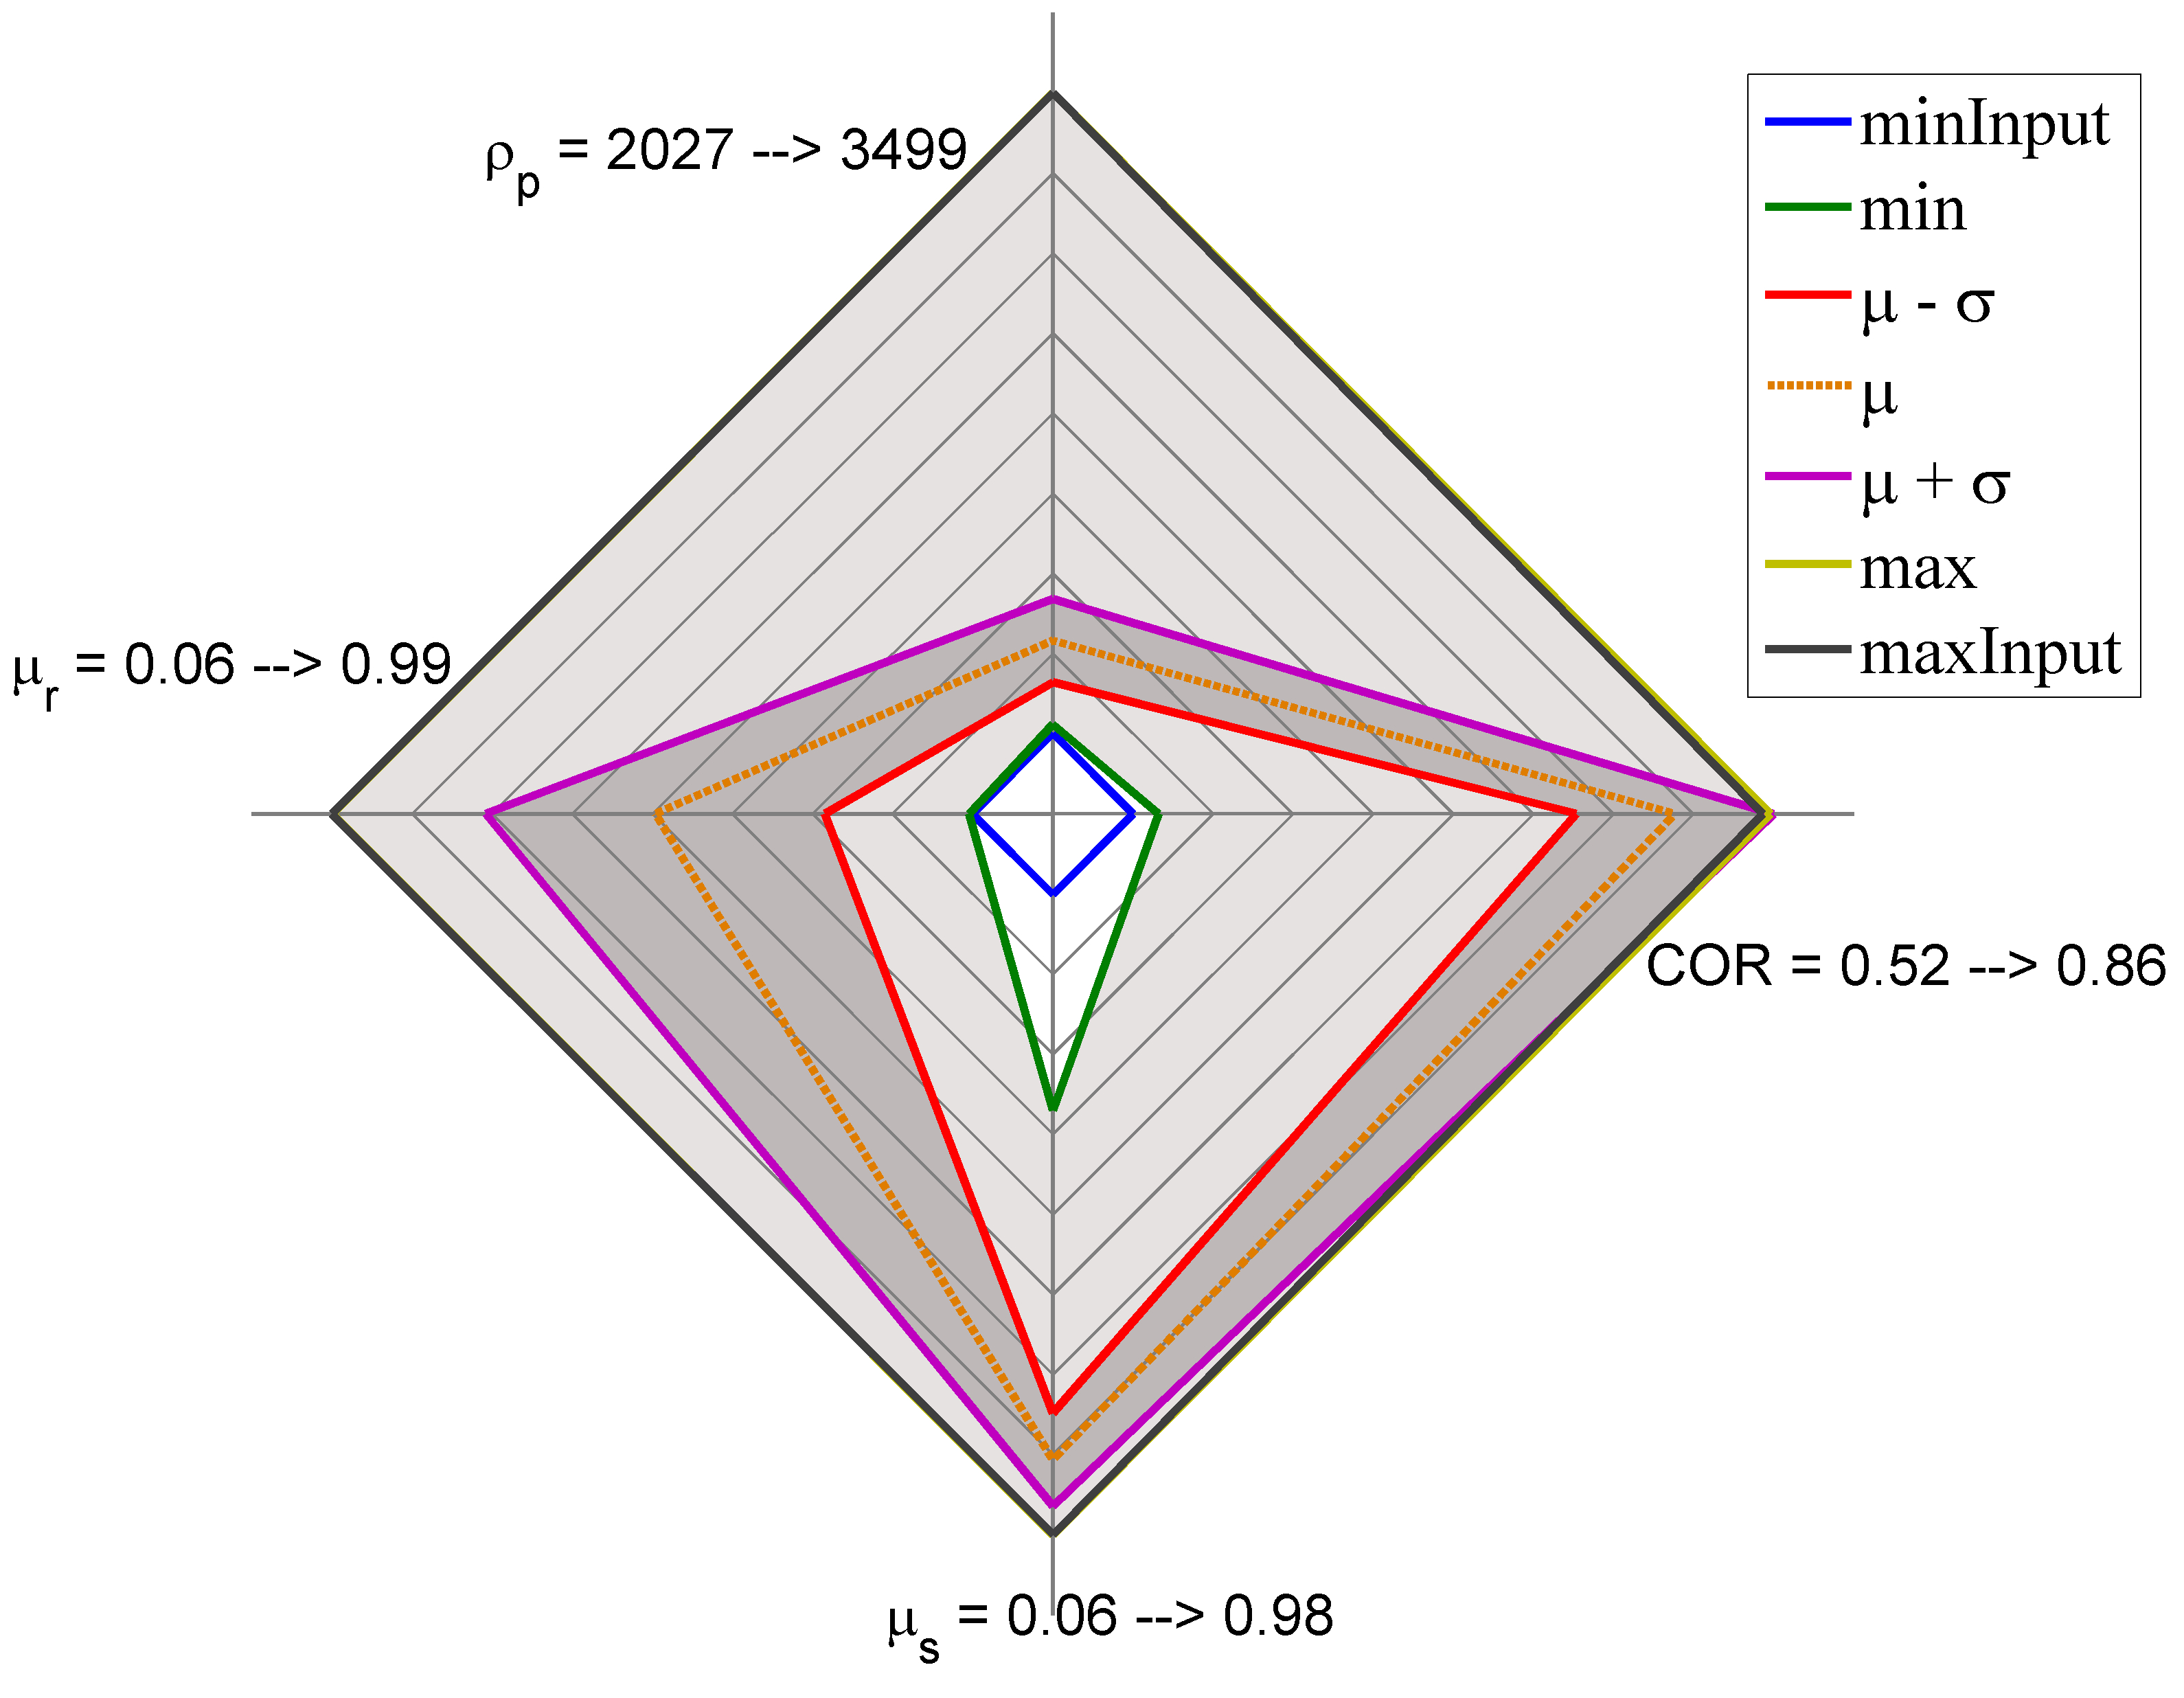
\includegraphics[height=3in]{images/original/28radarpirker12schulze10070}
%[width=.96\textwidth]
\caption{Radar P12 Schulze10070}
\label{fig:28radarpirker12schulze10070} 
\end{figure}

%SCT: sn = 10070 [Pa], coeff. P. = 1.2
% \begin{figure}[htp]
%     \centering
%     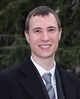
\includegraphics[width=.2\textwidth]{images/vitae/lbenvenuti}
%     \caption{OpenMP, MPI, MPI/OpenMP Hybrid runs of Box in a box testcase on 32
%     cores. The OpenMP-only run suffers from limited memory bandwidth in
%     memory-bound algorithms inside of the Modify section of the code. MPI-only has
%     low averaged runtimes for each section, but a very large Other timing, which
%     hints for a large amount of load-imbalance. Hybrid timings are a bit worse
%     on average, but because of better balancing, processes have lower wait times
%     inside of Other timing.}
% 	\label{fig:boxInBoxComparison}

% \ref{eq:rsquare}.
% \begin{equation}
R^2 = \frac {SSR}{SST} = 1 - \frac {SSE}{SST} .
 \label{eq:rsquare}
\end{equation}

% 
% \ref{eq:rootMeanSquareError}.
% \begin{equation}
RMSE = \sqrt{\frac{\sum _{i=1}^{n} (x_{i}-\widehat{x}_{i})^{2}}{n}}
\label{eq:rootMeanSquareError}
\end{equation}



% \lipsum[1]
% \begin{equation}
m \ddot{x}_{ij} + c \dot{x}_{ij} + k x_{ij} =  F_{ij} .
\label{equ:newtonlaw}
\end{equation}

% \subsection{ANN identification}
% \label{subsec:annmodeliden}
% \subsection{ANN application}
% \label{subsec:annapplication}
% 
% Later, each of these three trained $NN$ received as insertion $100M$ different
% combinations $DEM-micro$ parameters.
% So, we gained the numerical bulk behavior for each of this combination. 
% We then compared the values of these behaviors against the experimental bulk
% values, $SRSCT$ and $AOR$, obtaining a narrow range of valid DEM-micro
% combinations (about 80K).
% These results have been showed through radar plots (Figs. \ref{fig:15Schulze}
% and \ref{fig:16aorSchulzeIntersectionWorking}).
% To highlight an eventual $clumping$ behavior, we also plot the results in a
% cloud shape, see Fig. \ref{fig:17aorSchulzeIntersectionCloudSFRFCOR}.
% 
% %\begin{figure}[!htb] 
\centering 
\includegraphics[width=1.0\textwidth]{images/original/14aorSchulzeIntersection} 
\caption{aor Schulze Intersection}
\label{fig:14aorSchulzeIntersection} 
\end{figure}


% \begin{figure}[htp]
%     \centering
%     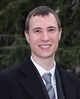
\includegraphics[width=.2\textwidth]{images/vitae/lbenvenuti}
%     \caption{OpenMP, MPI, MPI/OpenMP Hybrid runs of Box in a box testcase on 32
%     cores. The OpenMP-only run suffers from limited memory bandwidth in
%     memory-bound algorithms inside of the Modify section of the code. MPI-only has
%     low averaged runtimes for each section, but a very large Other timing, which
%     hints for a large amount of load-imbalance. Hybrid timings are a bit worse
%     on average, but because of better balancing, processes have lower wait times
%     inside of Other timing.}
% 	\label{fig:boxInBoxComparison}

% \begin{figure}[!htb] 
\centering 
\includegraphics[width=.8\textwidth]{images/original/15Schulze} 
\caption{aor Schulze Intersection}
\label{fig:14aorSchulzeIntersection} 
\end{figure}


% \begin{figure}[htp]
%     \centering
%     \includegraphics[width=.2\textwidth]{images/vitae/lbenvenuti}
%     \caption{OpenMP, MPI, MPI/OpenMP Hybrid runs of Box in a box testcase on 32
%     cores. The OpenMP-only run suffers from limited memory bandwidth in
%     memory-bound algorithms inside of the Modify section of the code. MPI-only has
%     low averaged runtimes for each section, but a very large Other timing, which
%     hints for a large amount of load-imbalance. Hybrid timings are a bit worse
%     on average, but because of better balancing, processes have lower wait times
%     inside of Other timing.}
% 	\label{fig:boxInBoxComparison}

% % \lipsum[1]
% \begin{figure}[!htb] 
\centering 
\includegraphics[width=.96\textwidth]{images/original/16aorSchulzeIntersectionWorking} 
\caption{aor Schulze Intersection working}
\label{fig:16aorSchulzeIntersectionWorking} 
\end{figure}


% \begin{figure}[htp]
%     \centering
%     \includegraphics[width=.2\textwidth]{images/vitae/lbenvenuti}
%     \caption{OpenMP, MPI, MPI/OpenMP Hybrid runs of Box in a box testcase on 32
%     cores. The OpenMP-only run suffers from limited memory bandwidth in
%     memory-bound algorithms inside of the Modify section of the code. MPI-only has
%     low averaged runtimes for each section, but a very large Other timing, which
%     hints for a large amount of load-imbalance. Hybrid timings are a bit worse
%     on average, but because of better balancing, processes have lower wait times
%     inside of Other timing.}
% 	\label{fig:boxInBoxComparison}

% % \begin{equation}
\begin{aligned}
\phi_{e-psh} &= \arctan \left(\frac{\tau_{psh}}{\sigma_{n,psh}} \right) ,\\
\mu_{psh} &=\tan(\phi_{e-psh}) .
\end{aligned}
 \label{eq:phi_ps}
\end{equation}

% \begin{figure}[!htb] 
\centering 
\includegraphics[width=.96\textwidth]{images/original/17aorSchulzeIntersectionCloudSFRFCOR} 
\caption{Cloud aor Schulze Intersection working}
\label{fig:17aorSchulzeIntersectionCloudSFRFCOR} 
\end{figure}


% \begin{figure}[htp]
%     \centering
%     \includegraphics[width=.2\textwidth]{images/vitae/lbenvenuti}
%     \caption{OpenMP, MPI, MPI/OpenMP Hybrid runs of Box in a box testcase on 32
%     cores. The OpenMP-only run suffers from limited memory bandwidth in
%     memory-bound algorithms inside of the Modify section of the code. MPI-only has
%     low averaged runtimes for each section, but a very large Other timing, which
%     hints for a large amount of load-imbalance. Hybrid timings are a bit worse
%     on average, but because of better balancing, processes have lower wait times
%     inside of Other timing.}
% 	\label{fig:boxInBoxComparison}

